% Options for packages loaded elsewhere
\PassOptionsToPackage{unicode}{hyperref}
\PassOptionsToPackage{hyphens}{url}
%
\documentclass[
]{book}
\usepackage{lmodern}
\usepackage{amsmath}
\usepackage{ifxetex,ifluatex}
\ifnum 0\ifxetex 1\fi\ifluatex 1\fi=0 % if pdftex
  \usepackage[T1]{fontenc}
  \usepackage[utf8]{inputenc}
  \usepackage{textcomp} % provide euro and other symbols
  \usepackage{amssymb}
\else % if luatex or xetex
  \usepackage{unicode-math}
  \defaultfontfeatures{Scale=MatchLowercase}
  \defaultfontfeatures[\rmfamily]{Ligatures=TeX,Scale=1}
\fi
% Use upquote if available, for straight quotes in verbatim environments
\IfFileExists{upquote.sty}{\usepackage{upquote}}{}
\IfFileExists{microtype.sty}{% use microtype if available
  \usepackage[]{microtype}
  \UseMicrotypeSet[protrusion]{basicmath} % disable protrusion for tt fonts
}{}
\makeatletter
\@ifundefined{KOMAClassName}{% if non-KOMA class
  \IfFileExists{parskip.sty}{%
    \usepackage{parskip}
  }{% else
    \setlength{\parindent}{0pt}
    \setlength{\parskip}{6pt plus 2pt minus 1pt}}
}{% if KOMA class
  \KOMAoptions{parskip=half}}
\makeatother
\usepackage{xcolor}
\IfFileExists{xurl.sty}{\usepackage{xurl}}{} % add URL line breaks if available
\IfFileExists{bookmark.sty}{\usepackage{bookmark}}{\usepackage{hyperref}}
\hypersetup{
  pdftitle={Documento Técnico N°2: Encuestas de Ocupación},
  pdfauthor={Dirección Nacional de Mercados y Estadísticas - Subsecretaría de Desarrollo Estratégico},
  hidelinks,
  pdfcreator={LaTeX via pandoc}}
\urlstyle{same} % disable monospaced font for URLs
\usepackage{longtable,booktabs}
\usepackage{calc} % for calculating minipage widths
% Correct order of tables after \paragraph or \subparagraph
\usepackage{etoolbox}
\makeatletter
\patchcmd\longtable{\par}{\if@noskipsec\mbox{}\fi\par}{}{}
\makeatother
% Allow footnotes in longtable head/foot
\IfFileExists{footnotehyper.sty}{\usepackage{footnotehyper}}{\usepackage{footnote}}
\makesavenoteenv{longtable}
\usepackage{graphicx}
\makeatletter
\def\maxwidth{\ifdim\Gin@nat@width>\linewidth\linewidth\else\Gin@nat@width\fi}
\def\maxheight{\ifdim\Gin@nat@height>\textheight\textheight\else\Gin@nat@height\fi}
\makeatother
% Scale images if necessary, so that they will not overflow the page
% margins by default, and it is still possible to overwrite the defaults
% using explicit options in \includegraphics[width, height, ...]{}
\setkeys{Gin}{width=\maxwidth,height=\maxheight,keepaspectratio}
% Set default figure placement to htbp
\makeatletter
\def\fps@figure{htbp}
\makeatother
\setlength{\emergencystretch}{3em} % prevent overfull lines
\providecommand{\tightlist}{%
  \setlength{\itemsep}{0pt}\setlength{\parskip}{0pt}}
\setcounter{secnumdepth}{5}
 %%% REFERENCIAS
        \usepackage{hyperref}
        % links del indice en negro; citas y URL en azul
        \hypersetup{colorlinks = true, urlcolor={blue}, 
        citecolor={blue}, linkcolor ={blue}}
\usepackage[spanish]{babel} % Idiomas en los que se escribe el documento. 
\usepackage{booktabs}
\usepackage{amsthm}

\usepackage[final]{pdfpages}

\makeatletter
\def\thm@space@setup{%
  \thm@preskip=8pt plus 2pt minus 4pt
  \thm@postskip=\thm@preskip
}
\makeatother
\let\oldmaketitle\maketitle
\AtBeginDocument{\let\maketitle\relax}
\ifluatex
  \usepackage{selnolig}  % disable illegal ligatures
\fi
\usepackage[]{natbib}
\bibliographystyle{apalike}

\title{Documento Técnico N°2: Encuestas de Ocupación}
\usepackage{etoolbox}
\makeatletter
\providecommand{\subtitle}[1]{% add subtitle to \maketitle
  \apptocmd{\@title}{\par {\large #1 \par}}{}{}
}
\makeatother
\subtitle{Propuestas metodológicas para las encuestas de ocupación en alojamientos turísticos}
\author{Dirección Nacional de Mercados y Estadísticas - Subsecretaría de Desarrollo Estratégico}
\date{25 de agosto de 2021}

\begin{document}
\maketitle


\includepdf[pages={1}, scale=1]{DT2Portada.pdf}
\newpage

\let\maketitle\oldmaketitle
\maketitle

{
\setcounter{tocdepth}{1}
\tableofcontents
}
\hypertarget{presentaciuxf3n}{%
\chapter*{Presentación}\label{presentaciuxf3n}}
\addcontentsline{toc}{chapter}{Presentación}

El presente documento, \textbf{Propuestas metodológicas para las encuestas de ocupación en alojamientos turísticos}, se enmarca en el proyecto de \href{https://armonizacion.yvera.tur.ar//}{Armonización de las Estadísticas de Turismo en las Provincias} de la \textbf{Dirección Nacional de Mercados y Estadística de la Subsecretaría de Desarrollo Estratégico del Ministerio de Turismo y Deportes}. El objetivo general de este proyecto es contribuir con propuestas metodológicas para los sistemas de estadísticas de turismo provinciales que orienten a producir indicadores provinciales básicos y comparables.

Además de este, se encuentran disponibles una serie de documentos técnicos que abordan otras problemáticas vinculadas a la producción de estadística de turismo:

\begin{itemize}
\item
  \href{https://dnme-minturdep.github.io/DT1_medicion_turismo/}{Documento Técnico \#1}: Conceptos y elementos básicos para la medición provincial de los turistas
\item
  \href{https://dnme-minturdep.github.io/DT3_registros_adminsitrativos/}{Documento Técnico \#3}: Descripción, análisis y utilización de los Registros Administrativos para la medición del Turismo
\item
  \href{https://dnme-minturdep.github.io/DT4_perfiles/}{Documento Técnico \#4}: Propuestas Metodológicas para las Encuestas de Perfil del Visitante
\item
  \href{https://dnme-minturdep.github.io/DT5_actividad_empleo/}{Documento Técnico \#5}: Medición de la contribución económica del turismo: actividad y empleo
\end{itemize}

\hypertarget{documento-tuxe9cnico-nuxba2---resumen}{%
\subsection*{Documento Técnico Nº2 - Resumen}\label{documento-tuxe9cnico-nuxba2---resumen}}
\addcontentsline{toc}{subsection}{Documento Técnico Nº2 - Resumen}

El propósito general del documento es presentar propuestas metodológicas que puedan ser aplicadas a los relevamientos de alojamientos turísticos en los distintos niveles de interés (municipales, aréas turística, provincias, regiones, etc).

Los objetivos específicos, asimismo, son:

\begin{itemize}
\item
  Exponer las principales situaciones problemáticasidentificadas en los relevamientos de alojamiento turísticos provinciales y locales.
\item
  Presentar propuestas y recomendaciones metodológicas aplicables a los relevamientos de alojamientos turísticos, para todas las etapas del estudio, desde su planteamiento inicial hasta la estimación de resultados.
\end{itemize}

En consecuencia, en el \textbf{Capítulo} \ref{encuesta} se presenta la definición de las encuestas o relevamientos de alojamientos turísticos, así como también las principales situaciones y dificultades identificadas en los diferentes relevamientos provinciales y locales.

En el \textbf{Capítulo} \ref{guiaencuesta} se propone una secuencia lógica de pasos que deberían seguirse para la implementación de una encuesta de alojamientos turísticos.

\hypertarget{encuesta}{%
\chapter{\texorpdfstring{\textbf{Encuestas}}{Encuestas}}\label{encuesta}}

\hypertarget{definiciones-y-problemas-generales}{%
\section{Definiciones y problemas generales}\label{definiciones-y-problemas-generales}}

Los alojamientos turísticos, es decir todos aquellos establecimientos que regular u ocasionalmente ofrecen hospedaje nocturno a los turistas, son un elemento central para el turismo, dada la importancia que revisten tanto para los visitantes como para la industria turística misma. Por esta razón, los establecimientos de alojamiento turístico ocupan un rol crucial en la medición de la actividad turística y, consecuentemente, las encuestas o relevamientos de ocupación de dichos establecimientos son la fuente de información turística más utilizada en los países y en otros niveles jurisdiccionales (regiones, provincias, departamentos, municipios, etc.).

Las encuestas o relevamientos de establecimientos de alojamiento turístico son un tipo de operativo que se realiza desde la perspectiva de la oferta, es decir, desde la información que brindan los prestadores del servicio. Los objetivos perseguidos pueden ser diversos, dependiendo de los propósitos de las instituciones encargadas de su realización. Sin embargo, en términos generales, estos objetivos suelen ser:

\begin{itemize}
\item
  conocer, en términos cuantitativos y cualitativos, la oferta de establecimientos que prestan alojamiento turístico;
\item
  conocer la disponibilidad de plazas y habitaciones;
\item
  conocer el nivel de ocupación y actividad de los establecimientos que prestan el servicio de alojamiento turístico;
\item
  cuantificar los pernoctes y viajeros hospedados;
\item
  clasificar la demanda según origen y permanencia -cantidad de noches que permanecieron alojados-;
\item
  dimensionar el nivel de empleo generado por esta actividad;
\item
  analizar las tarifas del sector.
\end{itemize}

La mayoría de las encuestas de alojamientos turísticos abordan a los establecimientos \textbf{pagos}, es decir, aquellos en los que el servicio de alojamiento debe ser abonado; por tanto se deja por fuera a los lugares que ofrecen hospedaje gratuito, dada la mayor dificultad de captación que poseen. Los establecimientos pagos son los hoteles, apart-hoteles, hosterías, hoteles residenciales, departamentos y casas de alquiler temporario, campings, y cualquier otro establecimiento que requiera un pago por el servicio de hospedaje. En cambio, los establecimientos gratuitos comprenden a las casas de familiares y/o amigos, segundas viviendas\footnote{Las segundas viviendas son aquellos inmuebles propios o alquilados en forma permanente que no constituyen la residencia habitual de un hogar. Cabe recordar que, de acuerdo a la última actualización de las Recomendaciones Internacionales para Estadísticas de Turismo, del año 2008, los viajes, con o sin pernocte, a las segundas viviendas son por definición turísticos, a excepción de cuando el motivo del viaje es ser empleado por una unidad económica con residencia en el destino.} y otros tipos de alojamientos no convencionales (conventos, predios religiosos -para retiros espirituales-, etc.).

Uno de los inconvenientes asociados a los relevamientos de establecimientos de alojamiento turístico es su escasa comparabilidad en términos de la categorización utilizada para clasificar los establecimientos, tanto en el plano internacional como en los niveles provinciales, departamentales y municipales. Esto se debe a la ausencia de un sistema clasificatorio común que permita el ordenamiento de los diferentes establecimientos dentro de categorías únicas. Según las Recomendaciones Internacionales para Estadísticas de Turismo \href{https://unstats.un.org/unsd/publication/seriesm/seriesm_83rev1s.pdf}{RIET} de la Organización Mundial de Turismo (OMT) y la Organización de las Naciones Unidas (ONU), la diversidad de servicios prestados en los diferentes países torna difícil la creación de categorías internacionalmente comparables, razón por la cual alienta a los países a generar sus propias agrupaciones para su aplicación en el plano nacional o sub-nacional. No obstante, esto tampoco resulta sencillo al interior de un país, más aún de uno tan diverso y extenso como Argentina, con usos y costumbres y marcos normativos provinciales muchas veces disímiles.

\hypertarget{encuestas-en-argentina}{%
\section{Encuestas en Argentina}\label{encuestas-en-argentina}}

En Argentina se llevan adelante diversos operativos de alojamientos turísticos, ya sea desde instituciones nacionales, provinciales o municipales.

Desde la esfera nacional, el Ministerio de Turismo y Deportes de la Nación (en adelante MINTURDEP) y el Instituto Nacional de Estadísticas y Censos (INDEC) conducen desde el año 2004, con una periodicidad mensual, la Encuesta de Ocupación Hotelera (EOH). La misma tiene el objetivo de medir el impacto del turismo internacional e interno sobre la actividad de los establecimientos hoteleros y para-hoteleros\footnote{Los tipos de establecimientos relevados son, dentro de los hoteleros, hoteles de 1 a 5 estrellas, apart-hoteles, moteles, hoteles boutique; y, dentro de los para-hoteleros, hoteles residenciales, hoteles sindicales, albergues (o hostels), cabañas (o bungalows), hospedajes, bed\&breakfast, hosterías, etc. No obstante, entre estos tipos de alojamiento no se consideran los de tamaño pequeño (con hasta 4 habitaciones o 12 plazas inclusive). Cabe señalar que este operativo excluye a otros alojamientos, como las viviendas de alquiler temporario, los campings, las segundas viviendas y las viviendas de familiares y/o amigos, y otros lugares de alojamiento de menor relevancia, dada la diferencia que presentan en la prestación de servicios con respecto a los establecimientos hoteleros y para-hoteleros.}, por medio de los siguientes indicadores: cantidad de plazas y habitaciones disponibles y ocupadas; tasa de ocupación en plazas y habitaciones; número de viajeros hospedados totales y según origen (argentinos, por provincia, o extranjeros, por país o región) y permanencia. La encuesta se realiza sobre una muestra compuesta por establecimientos de 49 de las localidades con mayor oferta hotelera y para-hotelera del país, dentro de las siete regiones turísticas definidas por el MINTURDEP\footnote{Estas regiones son: Ciudad de Buenos Aires, Provincia de Buenos Aires, Córdoba, Litoral (Corrientes, Chaco, Entre Ríos, Formosa, Misiones y Santa Fe), Norte (Catamarca, Jujuy, Salta, Santiago del Estero, Tucumán y La Rioja), Cuyo (Mendoza, San Juan, San Luis) y Patagonia (Chubut, La Pampa, Neuquén, Río Negro, Santa Cruz y Tierra Del Fuego).}. De este modo, con la EOH es posible realizar dos tipos de estimaciones: 1) resultados para cada una de las 49 localidades contempladas individualmente; 2) resultados regionales (con una cobertura aproximada del 80\% de las plazas de cada región) y a nivel total país (con una representatividad del 60\% de las plazas totales). Por último, una de las ventajas de este relevamiento radica en que se ejecuta utilizando la misma metodología a lo largo y ancho del país.

Desde una perspectiva provincial/municipal, las instituciones provinciales o municipales de turismo (Secretarías, Direcciones, etc.) también se encargan de medir la actividad de los alojamientos turísticos, mediante relevamientos que pueden ser:

\begin{itemize}
\item
  coordinados y ejecutados por las instituciones provinciales en todas o algunas localidades de la provincia;
\item
  coordinados por las instituciones provinciales pero ejecutados por las localidades de la provincia;
\item
  coordinados y ejecutados por las instituciones municipales.
\end{itemize}

En el último caso citado, la situación más habitual es que las instituciones provinciales se encarguen de centralizar la información generada por las localidades, para luego producir informes que sinteticen y analicen todos los datos obtenidos, aparte de los informes que elaboran las jurisdicciones locales. Sin embargo, al no existir una misma metodología implementada por las diferentes localidades de una provincia, estos resultados suelen estar expuestos a problemas de consistencia y comparabilidad.

\hypertarget{estado-de-situaciuxf3n-general-de-operativos}{%
\section{Estado de situación general de operativos}\label{estado-de-situaciuxf3n-general-de-operativos}}

En este apartado se analizan las situaciones más frecuentes que se presentan cuando se encaran relevamientos a establecimientos de alojamiento que merecen especial atención.

En primer lugar, se observa que los diversos relevamientos provinciales/ departamentales/ municipales tienen distinto \textbf{alcance en cuanto a la población bajo estudio}. En efecto, si bien la mayoría de las jurisdicciones abordan a los establecimientos que cuentan con \textbf{habilitación comercial,} algunas también estudian a los establecimientos cuya habilitación se encuentra \textbf{en trámite}. Adicionalmente, unas pocas provincias/departamentos/localidades incluyen también en su análisis a los establecimientos no habilitados comercialmente. Por otro lado, ya dentro de los establecimientos con habilitación comercial, algunas jurisdicciones acotan su mirada solamente a los establecimientos que han sido inscriptos en la entidad de turismo, mientras que otras abarcan tanto a los inscriptos como no inscriptos en la entidad de turismo\footnote{En el proceso de habilitación de un establecimiento de alojamiento turístico, el paso que sigue a la habilitación comercial es la inscripción del establecimiento en la correspondiente entidad de turismo (Secretaría, Sub-Secretaría, Dirección, etc.). Un número considerable de establecimientos omiten esta segunda instancia, quedando fuera de los registros de la entidad de turismo. De este modo, los relevamientos de alojamientos turísticos que analizan únicamente a los establecimientos registrados en los listados de las entidades de turismo, dejan de lado a un conjunto de unidades que podrían tener impacto en el comportamiento del sector.}. Estas diferencias en el alcance lógicamente conllevan dificultades de comparabilidad entre las diferentes jurisdicciones, sean éstas provinciales, departamentales o locales. Adicionalmente, debe tenerse en cuenta que al excluir del foco de análisis a parte de los establecimientos de alojamiento (p.e. los no habilitados comercialmente o los no inscriptos en las entidades de turismo), se pierde de vista el impacto que los mismos pudieran tener tanto en el sector turístico como en la dinámica económica de la unidad geográfica en cuestión.

En relación al \textbf{tipo de estudio}, la mayoría de las jurisdicciones intentan tener una cobertura total (censal) de la población objetivo, aunque en muchos casos se llevan adelante estudios muestrales. Sobre este aspecto, una de las situaciones observadas es que la selección de los establecimientos que conformarán la muestra se realiza sin seguir un criterio estadístico\footnote{El muestreo estadístico es aquel en el que todos los elementos de una población (en la mayoría de los casos, los alojamientos habilitados) tienen una probabilidad de selección conocida. En el muestreo al azar simple, que es el método de selección más sencillo, todas las unidades tienen la misma probabilidad de selección.}. De hecho, suele ocurrir que la muestra seleccionada en realidad esté integrada por establecimientos cuyos dueños o responsables sean los más predispuestos a responder, lo cual no constituye un criterio estadístico en la construcción de la muestra. Esto merece especial atención a la hora de analizar los resultados, dado que los datos surgidos de dicha muestra pueden no ser representativos en relación a la población en análisis.

En lo que al \textbf{trabajo de campo} compete, la periodicidad o frecuencia con la que se relevan los datos difiere entre las diferentes provincias, departamentos y/o municipios. En efecto, se observó que la periodicidad de toma del dato puede ser diaria, semanal, quincenal o mensual. A su vez, en los operativos que relevan datos con una frecuencia no diaria, la información recabada puede referir a todos los días del período analizado o solamente a algunos días del mismo. Para este último caso, es preciso considerar si se analizarán los datos únicamente sobre los días relevados o si los resultados obtenidos se expandirán a todos los días comprendidos en el período en cuestión.

En cuanto a \textbf{los indicadores}\footnote{Los indicadores pueden ser variables concretas (expresadas en la misma pregunta del cuestionario) o variables más complejas y, en ocasiones, con cierto nivel de abstracción. Estas últimas suelen combinar más de una variable concreta (p.e., porcentaje de ocupación en plazas, que combina plazas ocupadas y plazas disponibles).}, la forma en que son construidos (desde las preguntas del cuestionario hasta la fórmula de cálculo del mismo indicador), difiere entre las distintas jurisdicciones. Por ejemplo, para la construcción del indicador ``porcentaje de ocupación en plazas'' , calculado en casi todos los relevamientos de alojamientos (ya que algunos toman las habitaciones como referencia), los procedimientos son muy disímiles. Al momento del relevamiento, algunas jurisdicciones indagan la cantidad de plazas ocupadas de cada establecimiento cubierto, mientras que otras consultan directamente el porcentaje de ocupación en plazas a cada informante (responsable o dueño del alojamiento). En esta última forma de indagación se presenta el riesgo de que la aproximación al porcentaje alcanzada por el encuestado esté sesgada (por que la percepción del respondente puede estar afectada por lo ocurrido en los últimos días o en otra porción del periodo considerado, cuyo comportamiento puede ser diferente del resto). Por otra parte, puede ocurrir que alguna jurisdicción indague por el ``porcentaje de ocupación'' sin especificar si se trata de ocupación en plazas o habitaciones, quedando del lado del informante la interpretación de cuál es la unidad a la que refiere la pregunta. Por todo esto, siempre que sea posible, es más recomendable relevar cantidades (de plazas o habitaciones ocupadas) en lugar del porcentaje, dado que encierra menos probabilidades de error al momento de recabar información.

Al momento de la estimación de los indicadores, los procedimientos también son harto disímiles entre sí. Continuando con el ejemplo anterior, algunas jurisdicciones estiman el porcentaje de ocupación general en plazas calculando el promedio simple de los porcentajes de ocupación de todos los establecimientos considerados, ya sea porque se releva directamente el porcentaje de ocupación de los establecimientos o porque se lo construye luego de relevar la cantidad de plazas ocupadas y disponibles de cada establecimiento. Otras jurisdicciones, en cambio, obtienen la tasa de ocupación general en plazas sumando la cantidad de plazas ocupadas de todos los establecimientos considerados, y dividiendo el resultado de dicha operación por la cantidad total de plazas disponibles en esos establecimientos. Las mismas diferencias de cálculo se observan cuando se realizan estimaciones en distintos agrupamientos, como ser clase (hotel, apart hotel, b\&b, etc.), categoría (estrellas), modalidad (hotelería o para-hotelería) o ubicación (localidad, departamento, región, provincia). La primera forma de cálculo, que estima un promedio más general a partir de promedios parciales, diluye el peso o importancia que cada establecimiento y/o estrato tiene sobre la población total y sobre el agrupamiento que se quiere construir, al no considerar la cantidad de plazas totales disponibles sobre las que se construyó el porcentaje.

Para mayor comprensión del punto anterior, se cita el siguiente ejemplo. Un relevamiento considera dos establecimientos, uno con 200 plazas y otro con 50 plazas; asimismo, el primero declara un 50\% de ocupación (100 plazas), mientras que el segundo informa un 70\% de ocupación (35 plazas); el primer procedimiento de cálculo obtendría un 60\% como porcentaje general de ocupación (70\%+50\%)/2, mientras que el segundo estimaría un 54\% como porcentaje general de ocupación (100+35)/(200+50). Se observa, por lo tanto, que no basta con considerar solo los porcentajes parciales para calcular un porcentaje general de ocupación. Lo adecuado es estimar cuánto representa ese porcentaje sobre las plazas disponibles del total de establecimientos considerados. Por ello, el segundo procedimiento (el cual realiza las estimaciones a partir de valores absolutos) resulta ser el más adecuado.

En otro orden, un inconveniente común a todas las provincias, departamentos y/o municipios, es la \textbf{no respuesta} por parte de algunos dueños o responsables de establecimientos. Esto resulta en una cobertura de establecimientos menor a la planeada (ya sea en relevamientos censales como por muestreo). La no respuesta merece especial atención, ya que puede conducir a otro problema denominado \textbf{``sesgo de no respuesta''}. Éste consiste en la distorsión, dentro de la muestra o casos alcanzados, del peso que algún/os grupo/s específicos tenía/n originalmente en la población bajo estudio: por ejemplo, si el segmento de hoteles de 1 a 3 estrellas obtiene respuesta de muchos menos establecimientos que los esperados, este grupo quedaría con un peso relativo mucho menor al que tenía en la población bajo estudio, mientras que otros grupos adquirirían, en consecuencia, un peso relativo mayor en relación a la población\footnote{Cuando un grupo obtiene en la muestra o conjunto de casos un peso menor al que presentaba en la población, éste se encuentra \textbf{sub-representado}. Por el contrario, si cuenta con un peso mayor al de la población, el grupo está \textbf{sobre-representado}.}. En las investigaciones sobre aspectos socio-económicos es muy frecuente que los sujetos que no respondan presenten características similares entre sí, lo que genera un desbalance, que en ocasiones puede ser de gran magnitud, de un estrato o grupo que presentan ciertos rasgos comunes. Dados los efectos que puede causar la no respuesta, es preciso que se evalúe su magnitud e impacto\footnote{Al respecto, véase apartado 2.9. Procesamiento y análisis de la información.} en los resultados y que se generen procesos de imputación de resultados a los establecimientos sin respuesta (o bien, para el total del estrato).

Por último, merece la pena destacar que en los casos en que se observaron procedimientos de expansión de los resultados obtenidos, estos suelen ser lineales, no respetando el peso o importancia de cada estrato o grupo. En los casos analizados, el mismo consiste en aplicar, por ejemplo, el porcentaje de ocupación en plazas general obtenido en la muestra (o en el conjunto de establecimientos--para los censos) sobre el total de plazas disponibles en todos los establecimientos que conforman el universo de estudio, para luego estimar la cantidad de plazas ocupadas en la población total. Este procedimiento es lineal, en el sentido que realiza una expansión directa, sin evaluar si en los casos efectivamente relevados se produjo un desbalance de los estratos o grupos. En efecto, de haberse producido dicho desbalance, sería necesaria una expansión de los resultados por estrato.

Para más información de los informes de resultados, series estadísticas y la metodología, vistá:

\href{https://www.yvera.tur.ar/estadistica/info/encuesta-de-ocupacion-hotelera-eoh}{\textbf{Informes de prensa en Yvera}}

\href{http://datos.yvera.tur.ar/dataset/encuesta-ocupacion-hotelera-parahotelera-eoh}{\textbf{Data Abierta}}

\href{https://www.indec.gob.ar/ftp/cuadros/economia/eoh_aspectos_metodologicos.pdf}{\textbf{Doc metodológico}} \textbf{(INDEC)}

\hypertarget{guiaencuesta}{%
\chapter{\texorpdfstring{\textbf{Guía para una encuesta}}{Guía para una encuesta}}\label{guiaencuesta}}

En este capítulo se presenta el esquema lógico que debería seguir un relevamiento de alojamientos turísticos, desde el momento en que se plantean los objetivos hasta la obtención de los resultados finales. Estos pasos son, en definitiva, los mismos que se plantean en cualquier tipo de investigación socio-económica, pero por cuestiones de practicidad se optó por enfocarlos a los relevamientos de alojamientos. Cabe indicar que si bien se presentan las etapas de una investigación como una secuencia lógica, en la práctica estas etapas permanecen en diálogo constante.

\hypertarget{definiciuxf3n-de-los-objetivos-de-investigaciuxf3n}{%
\section{Definición de los objetivos de investigación}\label{definiciuxf3n-de-los-objetivos-de-investigaciuxf3n}}

En primer lugar, una encuesta de alojamientos turísticos (así como cualquier investigación) debe iniciarse con el planteo de los \textbf{objetivos}, entendiéndose a los mismos como los resultados a los que se pretende arribar mediante la investigación.

Los objetivos, a su vez, se subdividen en objetivos \textbf{generales} y \textbf{específicos}. Estos últimos constituyen propósitos específicos que se desprenden del propósito general del estudio. Por ejemplo, el objetivo general de un relevamiento hotelero puede ser conocer el nivel de actividad de los alojamientos turísticos, del que pueden desprenderse objetivos específicos como:

\begin{itemize}
\item
  estimar la tasa de ocupación en plazas y habitaciones;
\item
  conocer la cantidad de viajeros alojados en establecimientos hoteleros y para-hoteleros;
\item
  cuantificar la cantidad de pernoctes registrados en establecimientos hoteleros y para-hoteleros;
\item
  etc.
\end{itemize}

Es importante destacar que los objetivos deben ser claros, para así evitar desviaciones en el proceso de investigación, y viables, es decir, susceptibles de ser alcanzados. Adicionalmente, los objetivos planteados deben ser coherentes entre sí, ya sea en relación al objetivo general como con otros objetivos específicos.

En la mayoría de los operativos provinciales, el \textbf{objetivo primordial de la encuesta es conocer la tasa de ocupación hotelera en plazas y/o habitaciones y la cantidad de viajeros que recibió la provincia, departamento y/o municipio durante un período determinado} (mes, año, temporada estival o temporada invernal). Cabe mencionar que, a pesar de pretenderse estimar indicadores provinciales, en muchas ocasiones la cobertura geográfica no alcanza a todas las localidades de la provincia ni está diseñada de modo tal que sea representativa de toda la provincia. En tales casos, debe tenerse en cuenta que las estimaciones se limitan a esas localidades relevadas y que, si la decisión fuese realizar un análisis estrictamente provincial, tales resultados deben expandirse a toda la provincia, mediante los procedimientos correspondientes.

\hypertarget{definiciuxf3n-de-la-poblaciuxf3n-bajo-estudio-y-las-unidades-de-anuxe1lisis}{%
\section{Definición de la población bajo estudio y las unidades de análisis}\label{definiciuxf3n-de-la-poblaciuxf3n-bajo-estudio-y-las-unidades-de-anuxe1lisis}}

Ligada al planteamiento del propósito inicial de la investigación se encuentra la definición de cuál será la \textbf{población}\footnote{Si bien aquí se plantea indistintamente, algunos autores prefieren utilizar únicamente el término población, dado que consideran que el universo es ``un conjunto infinito de datos'' , que son aplicados a la población (Hernández Sampieri, Fernández Collado, Baptista Lucio, 1998).} \textbf{o universo bajo estudio}, entendiendo a ésta última como al conjunto de elementos que pretenden estudiarse. Definir la población bajo estudio implica tres pasos fundamentales:

\begin{itemize}
\tightlist
\item
  Establecer cuáles serán las \textbf{unidades de análisis}, es decir, los sujetos o elementos que serán objeto de estudio. En los relevamientos de alojamientos turísticos, las unidades de análisis pueden ser los establecimientos, las habitaciones y/o las plazas. Por ejemplo, si se contabilizan los turistas alojados en los establecimientos, las unidades de análisis serán los mismos establecimientos. Si se estiman la cantidad o porcentaje de plazas ocupadas, las unidades de análisis serán las plazas. Por último, si se calculan la cantidad o porcentaje de habitaciones ocupadas, las unidades de análisis serán las habitaciones. Un mismo relevamiento puede tener varias unidades de análisis, ya que si, por ejemplo, se realizarán todas las estimaciones mencionadas previamente, las unidades serán tanto los establecimientos, como las plazas y habitaciones. Las unidades de análisis deben ser congruentes con los objetivos de estudio. En este sentido, a mayor claridad de los objetivos, mayor será la probabilidad de contar con unidades de análisis coherentes con ellos.
\end{itemize}

\hfill\break

\begin{itemize}
\tightlist
\item
  Definir la \textbf{cobertura geográfica} del relevamiento. En otras palabras, esto significa situar geográficamente a las unidades de análisis. La cobertura geográfica puede ser toda una provincia o algunas localidades de una provincia (por ejemplo, las que cuentan con mayor cantidad de plazas disponibles) o todo el ejido municipal, etc.
\end{itemize}

\hfill\break

\begin{itemize}
\tightlist
\item
  Delimitar \textbf{temporalmente} el estudio, lo que significa establecer el período al cuál estarán referidos los resultados \textbf{(el cuándo).} En este sentido, las mediciones pueden ser \textbf{continuas}, \textbf{puntuales} o \textbf{específicas}. Las mediciones continuas se realizan sistemática e ininterrumpidamente y suelen tener una cobertura total a lo largo de un año, independientemente de la periodicidad de los relevamientos (diario, semanal, quincenal, mensual, etc). Por otro lado, las mediciones puntuales, si bien son sistemáticas, se llevan a cabo en determinadas fechas (temporada alta y fines de semana largos, por ejemplo). Por último, las mediciones específicas suelen realizarse esporádicamente o por única vez, respondiendo a objetivos o situaciones particulares (por ejemplo, un evento o festividad de realización única).
\end{itemize}

Tomando en cuenta todo lo dicho, la población bajo estudio de un relevamiento de alojamientos turísticos podría estar constituida por todos los establecimientos (y sus correspondientes habitaciones y plazas) de las localidades más grandes (en términos de cantidad de plazas) de la provincia X, durante todo el año (es decir, en forma continua). Otro ejemplo podría plantear una población conformada por todos los establecimientos (y sus correspondientes habitaciones y plazas) inscriptos en la Secretaría de Turismo de la Provincia X, situados en todas las localidades de la jurisdicción provincial, durante las temporadas de verano, invierno y fines de semana largos.

\hypertarget{censo-o-muestra}{%
\section{¿Censo o Muestra?}\label{censo-o-muestra}}

Una vez establecido el universo bajo estudio (unidades de análisis, cobertura geográfica y temporal) es preciso definir el tipo de investigación a realizar, esto es si se abordará a todas y cada una de las unidades de la población bajo estudio o bien a una porción de la misma. En el primer caso se trata de un estudio de carácter \textbf{censal}, mientras que la segunda opción se refiere a un estudio por \textbf{muestreo}.

Si la elección fuese encarar una investigación que abarque a todas las unidades de la población, resulta necesario analizarla viabilidad de este alcance, en términos de costo y tiempo. En efecto, un censo insume más tiempo y representa mayores costos en relación a una encuesta por muestreo. Si se optase por realizar un estudio por muestreo, en tanto, debe tenerse presente que una muestra es un conjunto de unidades a partir de la cual se pretenden realizar inferencias sobre la población de origen. Por lo tanto, no cualquier subgrupo de la población podrá constituir una muestra cuyos resultados sean extrapolables a la totalidad de la población objeto.

En este sentido, si la decisión fuese realizar un estudio por muestreo, deben considerarse los siguientes puntos:

\begin{itemize}
\item
  la construcción de un marco muestral;
\item
  cuál será el procedimiento de selección de la muestra (o qué tipo de muestreo se llevará a cabo);
\item
  cuál será el tamaño de muestra apropiado para dar cuenta de los objetivos de la investigación.
\end{itemize}

Si bien una primera impresión podría considerar al censo como la opción más viable y sencilla, el mismo, además de sus implicancias en términos de costo y tiempo, puede ocasionar una serie de situaciones que podrían evitarse con una muestra. Por ejemplo, debido a la magnitud de un operativo censal, es probable que quienes ejecutan el relevamiento resignen calidad en las respuestas o en la forma de relevar en pos de terminar en el tiempo previsto el trabajo de campo. Este tipo de error es menos factible de presentarse en una encuesta por muestreo donde, si bien el resultado tendrá asociado un margen de error estadístico (conocido), la menor cantidad de casos a cubrir hace posible una mayor calidad en el registro de los datos. Por su parte, una muestra puede llevar implícito el riesgo de obtener resultados que no reflejen el comportamiento de la población. Sin embargo, si la muestra ha sido seleccionada con criterios estadísticos, será posible estimar el margen de error y el nivel de confianza de las estimaciones.

\textbf{Recomendación:} Como regla general, puede sostenerse que cuando el objetivo sea estudiar un pequeño número de unidades (por ejemplo, una localidad con menos de 30 establecimientos) lo más conveniente sea la realización de un estudio censal. En cambio, cuando el número de unidades sea elevado y/o se pretendan integrar varias localidades para obtener representatividad provincial, lo aconsejable es encarar un estudio por muestra.

La EOH cuenta con una muestra mensual de aproximadamente 3 mil establecimientos hoteleros y parahoteleros en las 49 localidades relevadas. El diseño es de tipo estratificado en grupos de establecimientos según categorías, con un método de selección de probabilidad proporcional a la cantidad de plazas. Es decir, los establecimientos de cada una de las localidades relevadas por la EOH tienen asociados una probabilidad de seleccion en función de las plazas que disponen dentro de cada estrato; aquellos hoteles con mayor cantidad de plazas ofrecidas tendrá mayor probabilidad de ser seleccionado en la muestra. Cabe aclarar, que los hoteles de 4 y 5 estrellas son de ``inclusión forsoza'' , es decir son censados todos. De esta manera, la EOH a partir de los datos muestrales expandidos brinda información mensual de 49 localidades, de 7 regiones turísticas y para el total nacional. Ver +: \href{https://www.indec.gob.ar/ftp/cuadros/economia/eoh_aspectos_metodologicos.pdf}{Doc metodológico} (INDEC).

\hypertarget{padruxf3n-de-establecimientos-de-alojamiento-turuxedsticos}{%
\section{Padrón de establecimientos de alojamiento turísticos}\label{padruxf3n-de-establecimientos-de-alojamiento-turuxedsticos}}

Un requisito fundamental en todo relevamiento de alojamientos turísticos, sea censal o muestral, es contar con un padrón o listado que contenga la totalidad de los establecimientos de alojamientos que cumplan, como mínimo, con las condiciones definidas para la población o universo bajo estudio. En efecto, dicho padrón operará como marco de referencia para la identificación de las unidades a ser relevadas. En el caso particular de los estudios por muestreo, el padrón de establecimientos constituye el marco muestral desde el cual se seleccionarán los establecimientos que conformarán la muestra a ser relevada.

A priori, la definición de la población o universo bajo estudio debería ser un paso previo a la selección del padrón. Sin embargo, en la práctica, en muchas ocasiones el alcance del padrón suele condicionar la delimitación del universo o población bajo estudio. De este modo, la población o universo ya no se desprende únicamente de los objetivos de estudio, sino que también depende de la información disponible en el padrón o listado.

En las provincias, departamentos y municipios, los alcances de los relevamientos son diversos, debido tanto a los objetivos de estudio propios de cada jurisdicción como a la cobertura del padrón.~

En relación a los objetivos, la mayoría de las jurisdicciones relevan únicamente a los establecimientos \textbf{con habilitación comercial} (dejando fuera de objeto a los establecimientos no habilitados), en tanto que otras incluyen también a los establecimientos con \textbf{habilitación en trámite}. Asimismo, unas pocas provincias, departamentos y/o municipios también cubren a los \textbf{establecimientos sin habilitación comercial.}

En lo que respecta a los padrones (o listados) de los que disponen las entidades de turismo de los distintos niveles jurisdiccionales, se suelen presentar las siguientes situaciones, que dependen en gran medida del proceso de habilitación y registro de los establecimientos de alojamiento turístico:

\textbf{Padrones o listados municipales:} Debido a que la habilitación comercial de los establecimientos de alojamiento se efectúa a nivel municipal, los listados de los que disponen las entidades municipales abarcan generalmente a la totalidad de los establecimientos habilitados.

\textbf{Padrones o listados provinciales:} Como regla general, todos los establecimientos habilitados comercialmente a nivel municipal deberían estar registrados en los padrones de las entidades provinciales de turismo, ya que su posterior registro en la entidad provincial es un procedimiento obligatorio. Sin embargo, a menudo esto no ocurre, razón por la cual los registros provinciales de establecimientos, salvo excepciones, suelen tener menor cantidad de establecimientos que los registros o listados municipales. Por tanto, suelen encontrarse discrepancias entre los padrones de los diferentes municipios que integran una provincia y el correspondiente registro provincial. En relación a este punto, hay algunas provincias que se encargan de completar su padrón provincial con los establecimientos que están presentes en el listado municipal, pero que no figuran en el listado oficial provincial. Sin embargo, estos casos son excepcionales.

Como consecuencia de estas situaciones, aquellas provincias que relevan (en su encuesta o relevamiento de alojamientos turísticos) únicamente aquellos establecimientos presentes en su registro provincial, no solo estarán excluyendo de su objeto de estudio a los establecimientos no habilitados, o con habilitación en trámite, sino que también estarán dejando fuera de análisis a aquellos establecimientos que, aun contando con habilitación comercial, no están asentados en los registros provinciales. En cambio, aquellas provincias que centralizan datos producidos por los municipios es posible que cuenten con una cobertura mayor de establecimientos habilitados, ya que los establecimientos relevados son los que figuran en los registros municipales; sin embargo, estarán dejando de lado a los establecimientos que no cuentan con habilitación comercial, y por tanto su cobertura no es total.

Una consecuencia no menor de las diferencias de cobertura de los padrones o listados de las diferentes provincias y municipios es la escasa comparabilidad interprovincial (e intermunicipal) de los resultados provenientes de este tipo de relevamientos.

\textbf{Recomendación:} Teniendo todo esto en cuenta, si se pretende tener una dimensión total del nivel de actividad de los establecimientos de alojamiento turístico, así como de la cantidad de viajeros estimados a partir de este tipo de relevamientos, es preciso tener una cobertura de establecimientos lo más amplia posible. En este sentido, en primer lugar, si bien los establecimientos no habilitados desarrollan su actividad obviando requerimientos legales, a los fines estadísticos es de relevancia incorporar a estos establecimientos dentro de la población bajo estudio. En segundo lugar, ya dentro de los establecimientos habilitados, es recomendable que los registros provinciales sean ampliados, tomando como referencia los registros municipales, que en general cuentan con mayor cantidad de establecimientos que los provinciales.

Por otro lado, los \textbf{procedimientos de actualización} también contribuyen a ampliar la cobertura de los padrones y, por tanto, de los relevamientos o encuestas de alojamientos turísticos. Por ello, \textbf{se recomienda desarrollar acciones para actualizar los padrones con una frecuencia adecuada.}

Mantener actualizados los padrones supone:

\begin{enumerate}
\def\labelenumi{\arabic{enumi})}
\item
  Tener registradas las altas y bajas de los establecimientos o lugares de alojamiento, y que esas situaciones sean fácilmente identificables al leer el padrón. Por ejemplo, si un establecimiento X cierra definitivamente, es aconsejable mantener el nombre del mismo en el padrón y agregarle alguna indicación que dé cuenta de su situación actual. Si, citando otro ejemplo, un establecimiento cierra sus puertas en forma temporaria, también es recomendable dejarlo asentado en el padrón, en forma similar a como se haría en los casos de cierre definitivo.
\item
  Para cada establecimiento o lugar de alojamiento, detallar la cantidad de habitaciones y/o unidades, y plazas disponibles. En este punto es preciso considerar que la disponibilidad en los establecimientos puede ser variable a lo largo de un año calendario, como consecuencia de la estacionalidad de la actividad turística u otros factores (por ejemplo, refacciones). Por ejemplo, puede ocurrir que durante las temporadas bajas, algunos establecimientos decidan sacar de la oferta algunas habitaciones (y por ende plazas) dada la menor demanda potencial de alojamiento durante dicho período o bien colocar una menor cantidad de camas en las habitaciones (manteniendo la cantidad de habitaciones pero disminuyendo las plazas disponibles). En este sentido, las jurisdicciones que actualizan con una alta frecuencia sus padrones (por ejemplo, mensualmente), probablemente tengan registradas estas situaciones. En cambio, aquellas jurisdicciones que actualicen el listado con menor frecuencia (por ejemplo, al inicio de cada temporada, anualmente, o, incluso únicamente al momento de la inscripción del establecimiento en el padrón o listado) es probable que no puedan tener una detección precisa de la variabilidad en la disponibilidad. A los fines de contar con padrones que reflejen lo más preciso posible la disponibilidad real de los establecimientos, lo recomendable es actualizar los padrones en forma continua a lo largo de todo el año. Una forma de lograr una actualización continua es solicitando la disponibilidad de plazas y habitaciones en el mismo relevamiento de ocupación de alojamientos. Por otro lado, es preciso que, en cada establecimiento listado, la cantidad de plazas registrada sea coherente con la cantidad de habitaciones registrada (p.e, la cantidad de plazas disponibles no puede ser inferior a la cantidad de habitaciones o unidades disponibles).
\item
  Ligado al aspecto anterior, para el caso de padrones conformados por establecimientos (o lugares de alojamiento) habilitados y no habilitados, es aconsejable que se explicite la situación en que se encuentran. Asimismo, si los padrones incluyen a los establecimientos (o lugares de alojamiento) con habilitación en trámite, es recomendable indicar cuál es el tiempo aproximado que lleva completar el trámite de habilitación. De este modo, si un establecimiento figura en situación de ``habilitación en trámite'' por un tiempo extendido, sería posible conjeturar si esa situación se debe a una demora administrativa o a un problema de actualización del padrón.
\end{enumerate}

Las implicancias planteadas representan un estado ideal de actualización, que en la situación particular de cada provincia/departamento/municipio pueden ser más o menos alcanzables. Lógicamente, padrones actualizados garantizan universos más completos y muestras más acordes a la población de que son extraídas, y por tanto, resultados de ocupación del sector con mayor robustez y representatividad.

\hypertarget{estudios-por-muestreo.-tipos-de-muestreo}{%
\section{Estudios por muestreo. Tipos de muestreo}\label{estudios-por-muestreo.-tipos-de-muestreo}}

Existen distintos tipos de muestreo. Un primer criterio de clasificación los distingue en \textbf{probabilísticos} y \textbf{no probabilísticos}. En el primer tipo de muestreo se tiene conocimiento de cada una de las unidades que conforman la población bajo estudio (y de la que se extraerá la muestra), ya que se dispone de algún documento u otro tipo de material que da cuenta de la misma. A su vez, al conocer a todas las unidades que conforman la población, también se conoce la probabilidad de cada una de ellas de ser seleccionadas para formar parte de la muestra. En cambio, en el muestreo no probabilístico no se dispone de información acerca de la población bajo estudio y, por ende, tampoco de las probabilidades de selección de cada unidad.

Teniendo en cuenta esta primera clasificación, y en caso que se haya optado por realizar un estudio por muestreo, el paso siguiente consiste en decidir qué tipo de muestreo se seguirá: probabilístico o no probabilístico.

\hypertarget{muestreo-no-probabiluxedstico}{%
\subsection{Muestreo no probabilístico}\label{muestreo-no-probabiluxedstico}}

El muestreo no probabilístico suele utilizarse cuando no se dispone de información acerca de la población bajo estudio y, por lo tanto, de los elementos que integrarán la muestra. Esta situación es muy habitual en las encuestas de demanda turística y perfil del visitante, en las que la obtención de un marco de muestreo adecuado presenta grandes dificultades. En los relevamientos de alojamientos turísticos, en cambio, los padrones de establecimientos ofrecen un listado con la identificación y otras informaciones de todos (o casi todos) los establecimientos que constituyen la población de estudio. Por lo tanto, es posible calcular la probabilidad de selección de cada establecimiento y, en consecuencia, sortear muestras probabilísticas.

Si bien en los relevamientos de alojamientos turísticos los padrones hacen posible seleccionar muestras probabilísticas, en el trabajo de campo, la misma puede devenir en no probabilística. Para comprender mejor esta situación, se cita el siguiente ejemplo. En un operativo se confecciona una muestra probabilística compuesta solamente por hoteles, clasificados en 5 grupos según categoría (estrellas), es decir, en hoteles de 5, 4, 3, 2 y 1 estrellas. En la misma, el peso de cada grupo de hoteles es proporcional al observado en la población; a su vez, las unidades de cada grupo son seleccionadas aleatoriamente. Durante el trabajo de campo, por falta de colaboración de los informantes, no se logra obtener información de varios hoteles de 3 estrellas; sin embargo, no se ejecuta ningún procedimiento de reemplazo de los establecimientos con no respuesta. Debido a ello la muestra se transformará en no probabilística, dado que, a causa de la no respuesta, las probabilidades de selección de los establecimientos dentro del grupo de 3 estrellas se han distorsionado. Esto no implica que la no respuesta de algunas unidades transformen a una muestra probabilística en no probabilística, pero sí que la magnitud de la no respuesta debe ubicarse dentro de parámetros razonables y que deben realizarse procedimientos - durante el trabajo de campo y después del mismo - para corregir los posibles sesgos que la no respuesta podría traer aparejados.

Cabe mencionar que la sola presencia de un padrón o registro de establecimientos no garantiza necesariamente que la muestra que de él se extraiga sea probabilística. Para que la muestra sea probabilística, en efecto, es preciso seguir algunos pasos, que serán descritos en los sub-apartados siguientes. Más aún, a pesar de la existencia de un padrón, puede ocurrir que alguna entidad de turismo decida seleccionar una muestra compuesta por los establecimientos cuyos informantes tengan mayor predisposición a responder. Una selección guiada por este criterio es un ejemplo de muestra no probabilística deliberada como tal.

Si bien el muestreo no probabilístico se constituye en una alternativa posible, el mismo presenta algunas desventajas en relación al probabilístico:

\begin{itemize}
\item
  La muestra que de él resulta puede estar sesgada (es decir, puede haber sobre-representación de algún grupo y/o sub-representación de otro grupo).
\item
  No es posible conocer el grado de precisión y el nivel de confianza de las estimaciones (estos conceptos serán desarrollados en los siguientes sub-apartados).
\item
  Vinculado al punto anterior, no es posible generalizar los resultados de la muestra a la población sino que solo serán representativos de los elementos incluidos en la muestra.
\end{itemize}

\textbf{Recomendación:} Más allá de las desventajas, el muestreo no probabilístico se presenta como una alternativa útil cuando no se cuenta con un marco muestral del cual seleccionar las unidades que conformarán la muestra. Sin embargo, tal como se mencionó previamente, esto no es algo que suceda en los relevamientos de alojamientos turísticos, ya que en todos los casos se cuenta con un marco de muestreo, por lo tanto no cabe duda de que este tipo de operativos deben contemplar las herramientas que la estadística y el muestreo brindan para construir estudios robustos y representativos.

Para cada localidad (dominio muestral) de la EOH, se diseña una muestra estratificada. Los estratos se construyen teniendo en cuenta la categoría de cada uno de los hoteles del marco. El tamaño muestral de cada uno de los estratos en cada localidad relevada se adjudica a través de una asignación óptima (a diferencia de la asignación proporcional, en este caso, la muestra recogerá más hoteles de aquellos estratos que tengan más variabilidad). Luego, teniedo los correspondientes tamaños para cada estrato, la selección de los hoteles será a través de un muestreo con probabilidad proporcional a la cantidad de plazas disponibles. Es decir, los hoteles con mayor oferta de plazas tendrá mayor probabilidad de selección para conformar la muestra de ese estrato.

\hypertarget{muestreo-probabiluxedstico}{%
\subsection{Muestreo probabilístico}\label{muestreo-probabiluxedstico}}

A diferencia del muestreo no probabilístico, las muestras probabilísticas son aquellas en las que:

\begin{itemize}
\item
  todas los elementos de la población \textbf{tienen alguna probabilidad} de ser seleccionados, siendo dicha probabilidad distinta a cero,
\item
  las probabilidades son \textbf{conocidas} de antemano, es decir, previo al sorteo de las unidades que finalmente compondrán la muestra.
\end{itemize}

En este tipo de muestras, la selección de los elementos que la integrarán sigue un procedimiento \textbf{aleatorio}, es decir, sin intervención de la subjetividad del investigador o de otras personas que puedan estar involucradas en esta etapa.

Cabe mencionar que únicamente las muestras probabilísticas son las que hacen posible la \textbf{inferencia estadística}, esto es, que los resultados obtenidos sean extrapolables a la población objeto de estudio, ya que permiten conocer el nivel de confianza y la precisión de esas estimaciones.

\hypertarget{marcos-muestrales}{%
\subsubsection{Marcos muestrales}\label{marcos-muestrales}}

Como se adelantó en párrafos anteriores, una condición prácticamente indispensable para poder llevar adelante un proceso probabilístico de selección de la muestra es contar con un \textbf{marco muestral}. Este último, en términos prácticos, es un listado que contiene la totalidad de las unidades que componen la población de estudio y que permite conocer, previo al sorteo (selección aleatoria) de la muestra, la probabilidad de selección de cada elemento.

En las encuestas de alojamientos turísticos, los listados que operan como marco muestral son, como ya se indicó, los padrones o listados de establecimientos de alojamiento.

La EOH cuenta con un marco muestral compuesto por la nómina de todos los establecimientos hoteleros y parahoteleros del país con sus principales características: categoría hotelera, número de habitaciones o unidades disponibles, número de plazas disponibles, servicios ofrecidos, etc. Todos los años este padrón se actualiza a través de la incorporación de los nuevos establecimientos que aparecen en las localidades relevadas y la baja de los establecimientos que dejan de existir. A partir de este registro se toman las muestras todos los años y se expanden los resultados de la misma. Cabe aclarar que en el marco solo se consideran los establecimientos que tengan más de 12 plazas o más de 4 habitaciones/unidades.

\hypertarget{muestreo-aleatorio-simple}{%
\subsubsection{Muestreo aleatorio simple}\label{muestreo-aleatorio-simple}}

El muestreo aleatorio simple (MAS) resulta ser el más sencillo de todos, pero, a la vez, el menos utilizado en la práctica de la investigación. No obstante ello, su análisis hace posible la comprensión de otros procedimientos de muestreo más complejos.

Un procedimiento de selección de muestra es aleatorio simple si otorga a cada elemento de la población objeto \textbf{la misma probabilidad} de ser seleccionado. Esta probabilidad de selección está definida por la razón entre n/N (fracción de muestreo), donde n es el tamaño deseado de la muestra y N el tamaño de la población.

Una forma adecuada de seleccionar una muestra con este procedimiento es enumerando a todos los elementos de la población (por ejemplo, a cada establecimiento del padrón de alojamientos habilitados) secuencialmente, desde 1 hasta N. Luego, se debe realizar una selección aleatoria de las unidades\footnote{Programas informáticos de uso muy difundido como el Excel contemplan una función generadora de números aleatorios. No obstante, el ``sorteo'' puede realizarse de cualquier forma, incluso manualmente, mientras se respete el criterio de completa aleatoriedad.}.

\hypertarget{muestreo-sistemuxe1tico}{%
\subsubsection{Muestreo sistemático}\label{muestreo-sistemuxe1tico}}

El muestreo sistemático (en adelante, MSYS) también asigna a cada elemento de la población idéntica probabilidad de selección (n/N), aunque el procedimiento difiere en relación al MAS.

En primer lugar, al igual que en el MAS, deben numerarse consecutivamente todos los elementos de la población, desde 1 hasta N. En segundo lugar, se procede a calcular la razón entre el tamaño poblacional (N) y el tamaño deseado de la muestra (n), N/n, que es denominado \textbf{intervalo de selección}. Por ejemplo, si la cantidad total de establecimientos de alojamiento en una localidad es de 1.800 y el tamaño de la muestra que se pretende seleccionar es de 180 establecimientos, el intervalo de selección será 10. En tercer lugar, debe seleccionarse un número aleatorio \textbf{(r)} entre 1 y 10, que será el que designe al elemento que dará arranque a la selección (denominado \textbf{arranque aleatorio}). Una vez seleccionada la unidad que ocupa el primer lugar, se debe tomar la siguiente, que está a 10 lugares de la primera (r+10), es decir, la que está en la posición 11. Sucesivamente, debe continuarse con la selección del resto de las unidades, respetando los intervalos de selección (en este ejemplo, 21, 31, 41, etc.).

Una de las ventajas de los MSYS es que permiten ordenar a la población de acuerdo a una variable conocida y relevante para el estudio (por ejemplo, cantidad de habitaciones o plazas, o categoría del establecimiento) y así garantizar una mejor representatividad de la muestra respecto a la población de origen. Esto es posible también, y con mayor rigurosidad, empleando un muestreo aleatorio estratificado por asignación proporcional (el caso más simple de muestreo estratificado, descrito en el apartado \protect\hyperlink{muestreo-estratificado}{Muestreo estratificado}). No obstante, el muestreo sistemático con una variable ordenadora es una excelente aproximación al muestreo estratificado y de mayor practicidad.

\hypertarget{tamauxf1o-de-la-muestra}{%
\subsubsection{Tamaño de la muestra}\label{tamauxf1o-de-la-muestra}}

Si bien se comenzó el desarrollo sobre muestras probabilísticas con los conceptos de MAS y MSYS, la \textbf{determinación del tamaño de la muestra} es un paso previo a la selección de los elementos que finalmente la conformarán.

El muestreo probabilístico presenta la ventaja de ofrecer fórmulas matemáticas que, con la ayuda de información sobre la población bajo estudio, permiten establecer el tamaño de muestra adecuado para los resultados que pretenden alcanzarse.

Adicionalmente, es necesario mencionar que, a pesar de existir fórmulas que permiten determinar el tamaño de la muestra, el procedimiento total no es ``automático'' , sino que deben contemplarse una serie de factores y circunstancias que permitirán luego definir cuál es el tamaño de muestra adecuado para el estudio específico.

En primer lugar, no deben perderse de vista los objetivos del estudio y los niveles de desagregación con que se pretende analizar la información (sub-dominios de análisis). En efecto, si el propósito del estudio fuese presentar los resultados abiertos por clase y categoría de los establecimientos, el tamaño final de la muestra debería permitir realizar dichas desagregaciones con casos suficientes para obtener estimaciones robustas.

Adicionalmente, el tamaño de la muestra también depende de con cuánta \textbf{precisión} quiera realizarse la estimación, dado que un estudio por muestra siempre llevará asociado un \textbf{margen de error estadístico}. Que una estimación tenga un margen de error no significa que sea ``incorrecta'' , sino que indica un rango, a partir del valor puntual obtenido, dentro del cual se encontrará el valor verdadero con un determinado grado de confianza. En otras palabras, el error muestral expresa la distancia máxima que puede haber entre la estimación realizada sobre la muestra y el valor real poblacional (parámetro).

El error estadístico se expresa de diversas maneras, aunque generalmente se presenta como un valor que se suma y se resta a la estimación puntual. Por ejemplo, si un relevamiento arroja que la tasa de ocupación hotelera es del \(75\%\), y a su vez el error es de +/- 3, esto significa que el valor poblacional (verdadero) puede variar entre \(72\%\) y \(78\%\) (dado que el 3 se suma y se resta a la estimación puntual).

El margen de error es un atributo definido por quien lleva a cabo la investigación: cuanto mayor sea la precisión esperada de una estimación, menor debe ser el margen de error a definir. Sin embargo, esto no es gratuito: \textbf{a menor margen de error pretendido, mayor será el tamaño de la muestra sobre la que se deberá trabajar}.

Conviene profundizar algo más en este tema con un ejemplo. Si el relevamiento tuviese como una de sus finalidades principales medir variaciones a lo largo del tiempo, debe considerarse un margen de error adecuado a la sensibilidad del cambio que se procura revelar con la investigación, puesto que desde un punto de vista estricto, puede afirmarse que hubo variaciones cuando los intervalos (estimación +/- margen de error) no se superponen. Así, si se trabaja con un margen de error de 3\% y en diciembre de 2012 se obtuvo una tasa de ocupación del \(60\%\)(intervalo \(57\%\)-\(63\%\)) y en diciembre de 2013 la estimación alcanzó al \(62\%\) (intervalo \(59\%\)-\(65\%\)), no puede concluirse que hubo una modificación en la variable estimada, puesto que los intervalos de confianza de los resultados obtenidos se superponen. En otras palabras, un estudio con un margen de error del 3\% permitirá afirmar que hubo variaciones estadísticamente significativas sólo cuando las diferencias superen los 6 puntos porcentuales.

Como puede deducirse, al establecer el margen de error con el que se trabajará se debe respetar la profundidad que la investigación requiere, o bien, reducir el alcance de los objetivos de la misma. Si bien siempre es preferible un margen de error más pequeño, lograrlo implica cada vez mayores costos (económicos, humanos, de tiempo), y por tanto es preciso analizar ventajas y desventajas para arribar a la definición a un nivel de error eficiente\footnote{Cabe señalar que los estudios censales carecen, por definición, de errores estadísticos. No obstante, existen otro tipo de errores que afectan a los resultados obtenidos, tanto por muestra como por censo y que se denominan ``errores no muestrales'' o ``errores no estadísticos'' y, a diferencia de los errores estadísticos es imposible (o harto complejo y muy costoso, en el mejor de los casos) estimar la magnitud de los mismos. El hecho de que muchas veces se realicen estudios por muestra se relaciona tanto con cuestiones operativas (menores costos) como con la posibilidad de reducir los errores no muestrales, al realizar un relevamiento de campo de mejor calidad centrado en pocas unidades, como se mencionó más arriba.}.

En cuanto a los condicionantes del tamaño de muestra, éste también depende del nivel de confianza con el que pretendan estimarse los indicadores. Habitualmente, en investigaciones socio-económicas se utilizan \textbf{niveles de confianza del} \(90\%\) \textbf{o} \(95\%\)\textbf{.} Un nivel de significación del \(90\%\) indica que, de 100 muestras que se extraigan del universo o población, en 90 de ellas se obtendrán estimaciones que expresarán el rango o intervalo en que se ubica el parámetro poblacional. Un nivel de confianza del \(95\%\), a su vez, indica probabilidades de acierto mayores, ya que de 100 muestras, 95 contendrán el valor del parámetro. Si bien el nivel de confianza también es definido por el investigador y, cuanto mayor sea la confianza definida, mayor será el tamaño de muestra, en este punto \textbf{se recomienda trabajar con un} \(90\%\) \textbf{de nivel de confianza}.

Por último, la \textbf{dispersión} de la población de origen, en función de la variable de estudio más relevante, también influye en el tamaño final que tendrá la muestra. Por dispersión se entiende a la variabilidad que presentan las diferentes unidades de una población en torno a una variable específica. Cuanto mayor sea la dispersión de la población, mayor será el tamaño de muestra necesario. Cabe señalar que en general se desconoce la dispersión en torno a la/s variable/s bajo estudio (dado que se desconoce la magnitud de los valores a estimar). Algunas alternativas que permitirían sortear esta situación podrían ser:

\begin{itemize}
\item
  tomar como referencia resultados de estudios previos;
\item
  realizar una prueba piloto, que arrojen un resultado posible de la variable a estimar;
\item
  suponer la máxima variabilidad posible.
\end{itemize}

Cabe señalar que existen diferentes fórmulas para determinar el tamaño de muestra, dependiendo de las estimaciones que pretendan realizarse a partir de la misma. Es decir, la fórmula será diferente según se procure estimar promedios, proporciones, totales, etc. En los relevamientos hoteleros, las estimaciones fundamentales que se recomienda realizar son las de cantidad de plazas ocupadas y cantidad de habitaciones/unidades ocupadas, para luego estimar proporciones o porcentajes (proporción multiplicada por 100). Por lo tanto, a priori se recomienda utilizar la fórmula para estimar totales (ya que se estimarán total de plazas o habitaciones/unidades ocupadas).

La fórmula para estimar totales, asumiendo un procedimiento de selección simple al azar (MAS), por ser el más sencillo, y en la que se asume que la población tiene un tamaño conocido (población finita), es:

\(n= (N2^*z2^*σ2)/ [d2+(N2^*z2^* σ2)/N) ]\), donde:

\(n\)= tamaño de la muestra;

\(z\)=valor estándar que depende del nivel de confianza fijado; para un nivel de confianza del \(90\%\), el valor de \(z\) es \(1,645\).

\(d\)=margen de error aceptado;

\(σ2\)=varianza de la población en torno a la variable de análisis. La varianza es una medida de la dispersión o variabilidad de la población alrededor de dicha variable. Por ejemplo, si la variable de análisis es plazas ocupadas, la variabilidad o dispersión depende de los diferentes valores que pueda asumir la variable en los diferentes establecimientos.

\(N\)=tamaño de la población.

Nótese que, entre la información de la que se necesita disponer para determinar el tamaño de la muestra, la más difícil de obtener es la de dispersión o variabilidad de la variable bajo estudio, ya que se supone que su comportamiento es desconocido. De hecho, el estudio por muestreo se estaría realizando justamente para conocer cómo se comporta dicha variable. Sin embargo, en muchas jurisdicciones es probable que se cuente con información de relevamientos previos, de los cuales pueda extraerse esta información. Asimismo, también existe la alternativa de recurrir a los datos de la EOH (del MINTURDEP-INDEC), que podrían aportar información sobre la dispersión de la variable en cuestión. Por último, una alternativa adicional, aunque menos recomendable que las anteriores (pero viable si no se puede optar por las mismas) podría ser emplear la fórmula para estimar proporciones, que también es una de las estimaciones a las que se arribaría, pero con el uso de las cantidades absolutas de plazas ocupadas. Esta fórmula, ante el desconocimiento de la dispersión de la población en torno a la variable de estudio, asume una máxima variabilidad, que equivale a considerar que la proporción a estimar será del 0,5.

La fórmula para estimar proporciones, asumiendo un procedimiento de selección simple al azar (MAS), y suponiendo que la población tiene un tamaño conocido (población finita), es:

\(n\) = \((z2^*p^*q)\) / \([d2 + (z2^*p^*q) / N]\), donde:

\(n\)= tamaño de la muestra;

\(z\)=valor estándar que depende del nivel de confianza fijado; para un nivel de confianza del \(90\%\), el valor de \(z\) es \(1,645\).

\(d\)=margen de error aceptado (\(3\%\)=\(0,03\), \(2\%\)=\(0,02\), etc.);

\(p\)=proporción a estimar (supuesto de máxima variabilidad=\(50\%\)=\(0,5\));

\(q\)=\(1-p\), también por definición \(0,5\) (\(1\)-\(0,5\)=\(0,5\));

\(N\)=tamaño de la población.

\hypertarget{la-representatividad-y-el-azar}{%
\subsubsection{La representatividad y el azar}\label{la-representatividad-y-el-azar}}

En investigación, es habitual referirse a si una muestra es o no ``representativa'' de la población o universo de la que fue seleccionada. A pesar de su uso frecuente, esta noción sólo tiene un alcance intuitivo, ya que no existe un procedimiento formal que permita medir el grado de representatividad de una muestra.

Sin embargo, a los fines de hacer un uso menos impreciso de este término, podría considerarse que una muestra es representativa cuando reproduce (o se aproxima a) la estructura de la población en torno a una o varias variables. En el caso de las encuestas de alojamientos turísticos, una muestra podría calificarse como representativa si, por ejemplo, en su interior la distribución de los tipos de alojamientos turísticos presenta la misma heterogeneidad que en el padrón.

Por otro lado, es común sostener que un procedimiento de selección al azar garantiza la obtención de una muestra representativa a los efectos de ciertos rasgos de la población (por ejemplo, el ``tipo'' de alojamientos: hoteles, hosterías, apart hoteles, etc.). Sin embargo, puede ocurrir, aunque no de manera frecuente (esta posibilidad se reduce a medida que se aumenta la muestra), que en una muestra seleccionada mediante MAS un grupo con ciertos rasgos presente en la misma un peso diferente al que tiene en la población. Por ejemplo, en la muestra, los apart hoteles pueden representar un \(8\%\) del total de establecimientos de alojamiento, mientras que en la población el peso es \(15\%\). En este caso, se está ante una situación de sub-representación del segmento apart hoteles; inversamente, también puede producirse una sobre-representación de los apart hoteles en relación a la población de referencia.

Por esta razón, emplear el procedimiento de selección sistemático mediante una variable ordenada es preferible, dado que previene contra casos de ``mala suerte'' en las unidades seleccionadas. En este sentido, un muestreo aleatorio estratificado por asignación proporcional es aún mejor, pero de difícil cálculo.

\hypertarget{muestreo-estratificado}{%
\subsubsection{Muestreo estratificado}\label{muestreo-estratificado}}

Como se adelantó, un procedimiento de selección que permite aproximarse a muestras representativas de la estructura poblacional es el muestreo aleatorio estratificado, dado que intenta reflejar, en la muestra, la composición poblacional en función de determinadas características que se asumen como relevantes para el tema bajo estudio.

Adicionalmente, el muestreo estratificado también responde a otras finalidades:

\begin{itemize}
\item
  Disminuir la dispersión general de la variable en estudio, mediante la conformación de grupos (o sub-poblaciones) homogéneos en su interior.
\item
  En relación al punto anterior, alcanzar resultados más precisos con un mismo tamaño de muestra. Por ejemplo, si con MAS se alcanzó un tamaño de muestra de 400 casos, que permitirá realizar estimaciones con un margen de error de +/- \(4\%\), mediante el muestreo estratificado es posible obtener resultados con un margen de error inferior a \(4\%\), manteniendo el mismo tamaño de muestra.
\item
  Obtener resultados en sub-poblaciones de interés. Por ejemplo, si la variable/s en torno a la/s cual/es se estratifican es/son clase y categoría, y, asimismo, se pretende realizar estimaciones para un grupo específico (p.e., hoteles de 5 estrellas), es recomendable considerar a este grupo como un estrato específico.
\end{itemize}

La estratificación es un proceso previo a la selección de las unidades que conformarán la muestra, que consiste en clasificar a la población bajo estudio en diferentes \textbf{grupos o estratos,} según características específicas que se supone tienen algún tipo de impacto en el comportamiento de la variable/s de análisis. En el caso específico de los relevamientos de alojamientos, los estratos suelen estar constituidos por ``clases de alojamiento'' (hotel, apart hotel, bungalow" , etc), ``categorías de alojamiento'' (estrellas), una combinación entre ambas, o bien, en el caso de estudios de alcance provincial, por distintas localidades, etc.

Estos estratos deben ser lo más homogéneos posible en su interior (es decir, las unidades que lo componen tienen que ser lo más parecidas entre sí) y lo más diferente posible del resto de los estratos (heterogeneidad externa), con el fin de lograr reducir la dispersión general de la variable bajo estudio. Obviamente, la homogeneidad interna y heterogeneidad externa estarán definidas en función de la variable de estratificación.

Es preciso tener presente que para poder estratificar a la población, es necesario tener un conocimiento previo de la misma. Por lo tanto, es indispensable que la información auxiliar que se utilizará para segmentar a la población esté presente en el marco muestral.

Luego de haberse establecido cuáles serán los estratos, se hace necesario \textbf{determinar el tamaño de cada estrato}, que en definitiva son sub-muestras dentro de la muestra total. A este procedimiento se le llama asignación de casos. Si bien existen diversas formas de asignar casos, aquí se presenta el proceso de \textbf{asignación proporcional}, que resulta ser el más sencillo de todos. Asimismo, tiene como ventaja el garantizar que la muestra reproducirá la estructura de la población en función de su distribución entorno a una o más variables. De este modo, se eliminaría el riesgo de una muestra aleatoria simple en la que la ``mala suerte'' deje por ejemplo a un grupo sin estimar.

\hypertarget{asignaciuxf3n-proporcional}{%
\paragraph{Asignación proporcional}\label{asignaciuxf3n-proporcional}}

Un paso previo a la asignación de casos es la determinación del tamaño total de la muestra. Una alternativa viable y sencilla es hacerlo mediante muestreo aleatorio simple (MAS), y posteriormente asignar casos a cada estrato.

Una vez establecido el tamaño total de la muestra, se procede a calcular el \textbf{peso relativo} (expresado en porcentaje o proporción) de cada uno de los estratos en la población total. Luego, el porcentaje o proporción correspondiente a cada estrato se multiplica por el tamaño total de la muestra, para obtener el tamaño (o cantidad de casos) de cada estrato. Por ejemplo, se supone que la población fue dividida en 3 estratos, cuyos pesos son 0,2, 0,45 y 0,35. Si el tamaño total de la muestra es de 400 casos, la cantidad de casos correspondiente a cada estrato será 80 (\(0,2\)*\(400\)), 180 (\(0,45\)*\(400\)) y 140 (\(0,35\)*\(400\)).

\hypertarget{procedimiento-de-selecciuxf3n-de-unidades-dentro-de-los-estratos}{%
\paragraph{Procedimiento de selección de unidades dentro de los estratos}\label{procedimiento-de-selecciuxf3n-de-unidades-dentro-de-los-estratos}}

Luego de haber definido los estratos y asignado un tamaño a cada uno de ellos, el paso siguiente es la selección de las unidades dentro de cada uno de ellos. Los métodos de selección pueden ser:

\begin{itemize}
\item
  \textbf{Muestreo Aleatorio Simple} (MAS), que asigna idéntica probabilidad de selección a cada elemento del estrato y en donde el azar determina la selección de cada unidad;
\item
  \textbf{Muestreo Sistemático}, que también adjudica idéntica probabilidad de selección, pero en donde se sigue un procedimiento sistemático de selección, con arranque aleatorio, ordenando previamente las unidades del universo de acuerdo a una variable relevante (por ejemplo, tamaño).
\end{itemize}

\textbf{Recomendación:} En virtud de lo expuesto, el \textbf{muestreo estratificado con asignación proporcional y proceso de selección sistemática} se revela como la mejor opción para las encuestas de usos de alojamientos turísticos, allí donde la población alcanza un tamaño destacado. En efecto, los padrones de establecimientos de alojamiento poseen variadas características conocidas (clase, categoría y/o ubicación) que permiten realizar una adecuada estratificación previa a la selección, y así obtener una muestra que refleje la variabilidad de la población de origen. Luego, en cada estrato, es recomendable ordenar a los establecimientos por su tamaño (cantidad de plazas o habitaciones) y extraer en forma sistemática las unidades que compondrán la muestra.

\hypertarget{otras-consideraciones-sobre-muestreo-estratificado}{%
\paragraph{Otras consideraciones sobre muestreo estratificado}\label{otras-consideraciones-sobre-muestreo-estratificado}}

En primer lugar, si bien se recomienda realizar relevamientos sobre muestras (dadas sus ventajas operativas y estadísticas), existen situaciones en donde se hace necesario un relevamiento de tipo censal. Es el caso de los estratos pequeños pero de gran importancia relativa, como ser los hoteles de alta categoría (4 y 5 estrellas), que es un criterio adoptado en la \href{https://www.indec.gob.ar/ftp/cuadros/economia/eoh_aspectos_metodologicos.pdf}{EOH}. Este estrato presenta un peso relativo pequeño dentro de la población bajo estudio, pero se supone que tiene un comportamiento diferencial con respecto al resto de los estratos. Por lo tanto, es estos casos se recomienda relevar a todos los establecimientos que forman parte del estrato (censo dentro del estrato), para garantizar una base robusta a partir de la cual realizar estimaciones.

Por otro lado, luego de haber asignado proporcionalmente los casos a cada estrato, puede que en alguno de ellos la cantidad de casos sea muy pequeña. En estos casos, es posible asignar mayor cantidad de casos a ese estrato (sin llegar a realizar un censo), con el fin de alcanzar una base de análisis que garantice estimaciones estadísticamente significativas para ese estrato.

Cabe mencionar que, en este último caso, al momento de construir los ponderadores (véase \protect\hyperlink{ponderadores-o-factores-de-expansiuxf3n}{Ponderadores o factores de expansión}), deberá contemplarse devolver a las unidades de dichos estratos el peso que originalmente tenían (es decir, aquel que corresponde a sus probabilidades de selección).

Para finalizar, como puede deducirse, la estratificación, en sí misma, no es un procedimiento de selección de unidades, sino que constituye un proceso previo a la selección de la muestra. Los procedimientos de selección de la muestra son los que ya se han desarrollado: MAS y Muestreo Sistemático.

\hypertarget{estratos-vs-dominios-de-anuxe1lisis}{%
\paragraph{Estratos vs dominios de análisis}\label{estratos-vs-dominios-de-anuxe1lisis}}

En este punto, es necesario aclarar que estrato no es sinónimo de sub-dominio de análisis, entendiendo a este último como una nueva base de análisis, aparte de la base total: p.e., hoteles de 4 y 5 estrellas, apart hoteles, etc. Sin embargo, a menudo existe una coincidencia entre estrato y sub-dominio de análisis. Ejemplificando, los hoteles de 3 estrellas junto a los apart hoteles y a los hoteles boutique pueden conformar un mismo estrato y, a la vez, constituir un sub-dominio de análisis. Lo que debe considerarse es que el fin último de la estratificación no es la definición de otras bases de análisis, además de la base total, sino:

\begin{enumerate}
\def\labelenumi{\alph{enumi})}
\item
  reflejar en la muestra la estructura poblacional, en torno a alguna variable que se juzgue relevante para el objetivo de estudio;
\item
  reducir la dispersión general de la población en torno a la variable de estudio que se considere más relevante para el estudio;
\item
  lograr mayor precisión en los resultados;
\item
  reducir el tamaño de muestra.
\end{enumerate}

Finalmente, si uno de los propósitos del estudio fuese analizar los resultados en sub-dominios de la población (p.e. si interesara conocer, además del total provincial de hoteles, los niveles de ocupación para la capital provincial por un lado, y para el resto de la provincia por otro, y dentro de cada uno de ellos, las diferencias entre los hoteles de alta categoría (4 y 5 estrellas) y el resto) es importante tener en consideración que estos sub-dominios deben surgir del agrupamiento de uno o más estratos, y que la cantidad de casos permita realizar estimaciones con un margen de error estadístico aceptable para los objetivos de la investigación).

\hypertarget{ejemplo-de-estratificaciuxf3n-y-selecciuxf3n-de-muestras-al-interior-de-cada-estrato}{%
\subsubsection{Ejemplo de estratificación y selección de muestras al interior de cada estrato}\label{ejemplo-de-estratificaciuxf3n-y-selecciuxf3n-de-muestras-al-interior-de-cada-estrato}}

La provincia X decide realizar un estudio de ocupación hotelera y parahotelera en algunas localidades que componen el territorio provincial. En cada una de las localidades seleccionadas (consideradas como estratos) el relevamiento será muestral. Se desea obtener resultados tanto para el conjunto de localidades como para cada localidad, sin diferenciar, al interior de estas, por tipo o categoría de los establecimientos.

En el ejemplo de la Figura \ref{fig:padronY}, se desarrollará el proceso de estratificación y selección de muestras dentro de cada estrato para una sola localidad en particular (localidad Y), que cuenta con el siguiente padrón de establecimientos:

\begin{figure}

{\centering 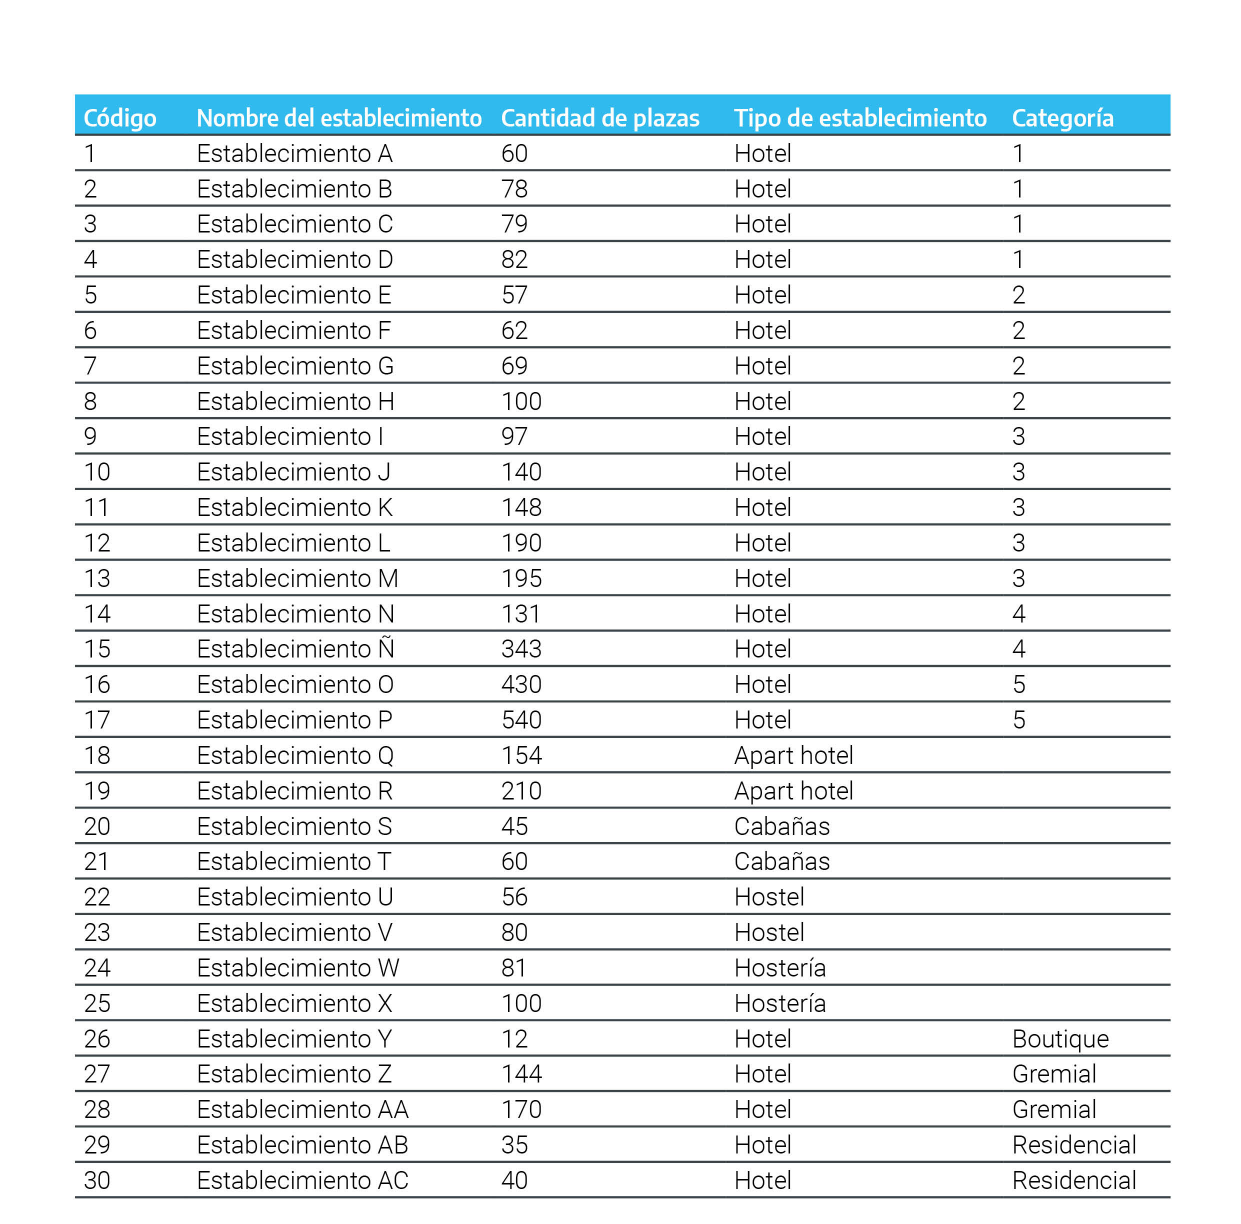
\includegraphics[width=1\linewidth]{imagenes/tabla_1} 

}

\caption{ Padrón de establecimientos de la localidad Y}\label{fig:padronY}
\end{figure}

\hypertarget{definiciuxf3n-de-los-estratos-en-la-localidad-y}{%
\paragraph{Definición de los estratos en la localidad Y}\label{definiciuxf3n-de-los-estratos-en-la-localidad-y}}

El primer paso, previo al proceso de selección, consiste en la definición de los estratos. Supóngase que la provincia X tiene conocimiento de que en la localidad en cuestión existe un comportamiento diferencial en cuanto a ocupación según la tipología, categoría del establecimiento y cantidad de plazas disponibles. Por tanto, se decide conformar lo siguientes estratos:

\begin{figure}

{\centering 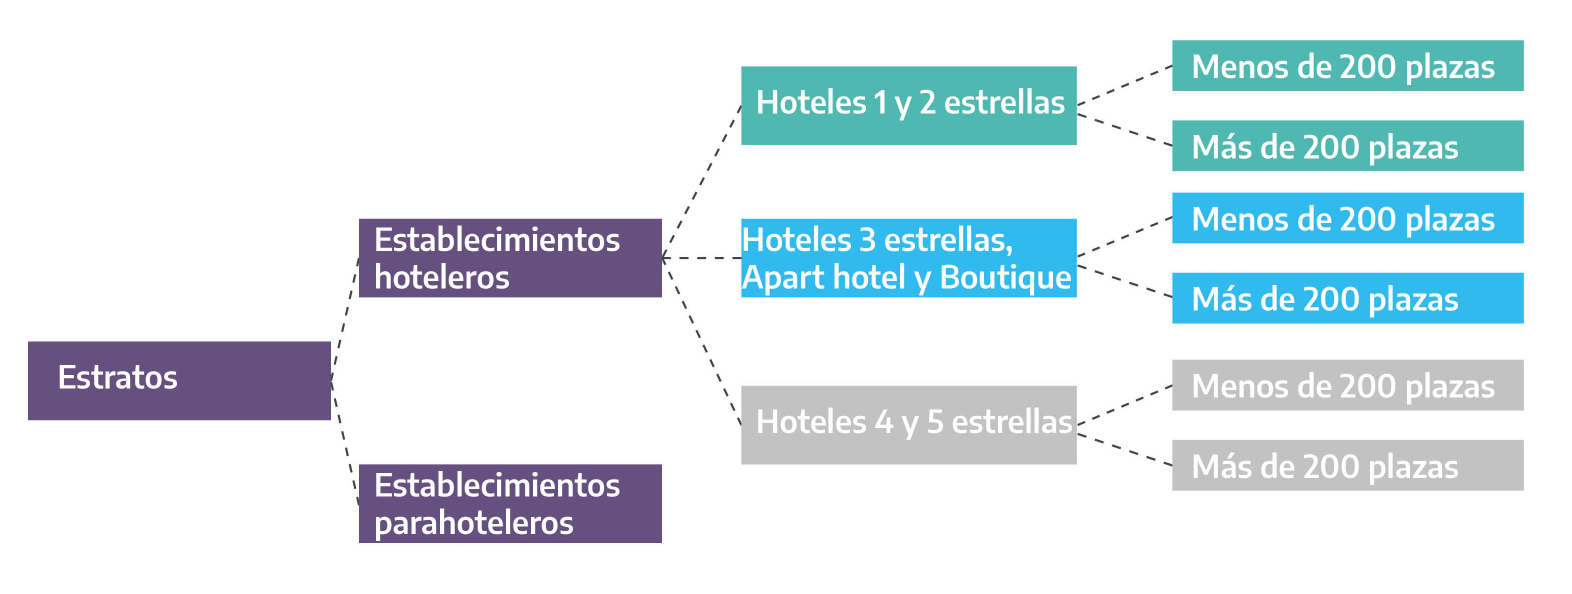
\includegraphics[width=1\linewidth]{imagenes/figura_1} 

}

\caption{ Estratos de establecimientos de la localidad Y}\label{fig:localidadY}
\end{figure}

Como se puede observar, un primer criterio de estratificación distingue a los establecimientos hoteleros y parahoteleros. Adicionalmente, un segundo criterio de estratificación segmenta a los establecimientos hoteleros en ``Hoteles 1 y 2 estrellas'' , ``Hoteles 3 estrellas, Apart hotel y Boutique'' y ``Hoteles 4 y 5 estrellas'' . Por último, un tercer criterio los diferencia entre si tienen menos o más de 200 plazas, ya que se supone que los establecimientos relativamente grandes (en función de la cantidad de plazas) manifiestan un comportamiento diferencial en relación a los de menor número de plazas. Nótese que el corte en menos o más de 200 plazas es totalmente arbitrario en este ejemplo; en la práctica de cada provincia, el criterio dependerá de las particularidades que manifieste el sector y, obviamente, de los objetivos del estudio.

Una vez definidos los estratos, se procede a clasificar los establecimientos del padrón en estos diferentes sub-universos.

\begin{figure}

{\centering 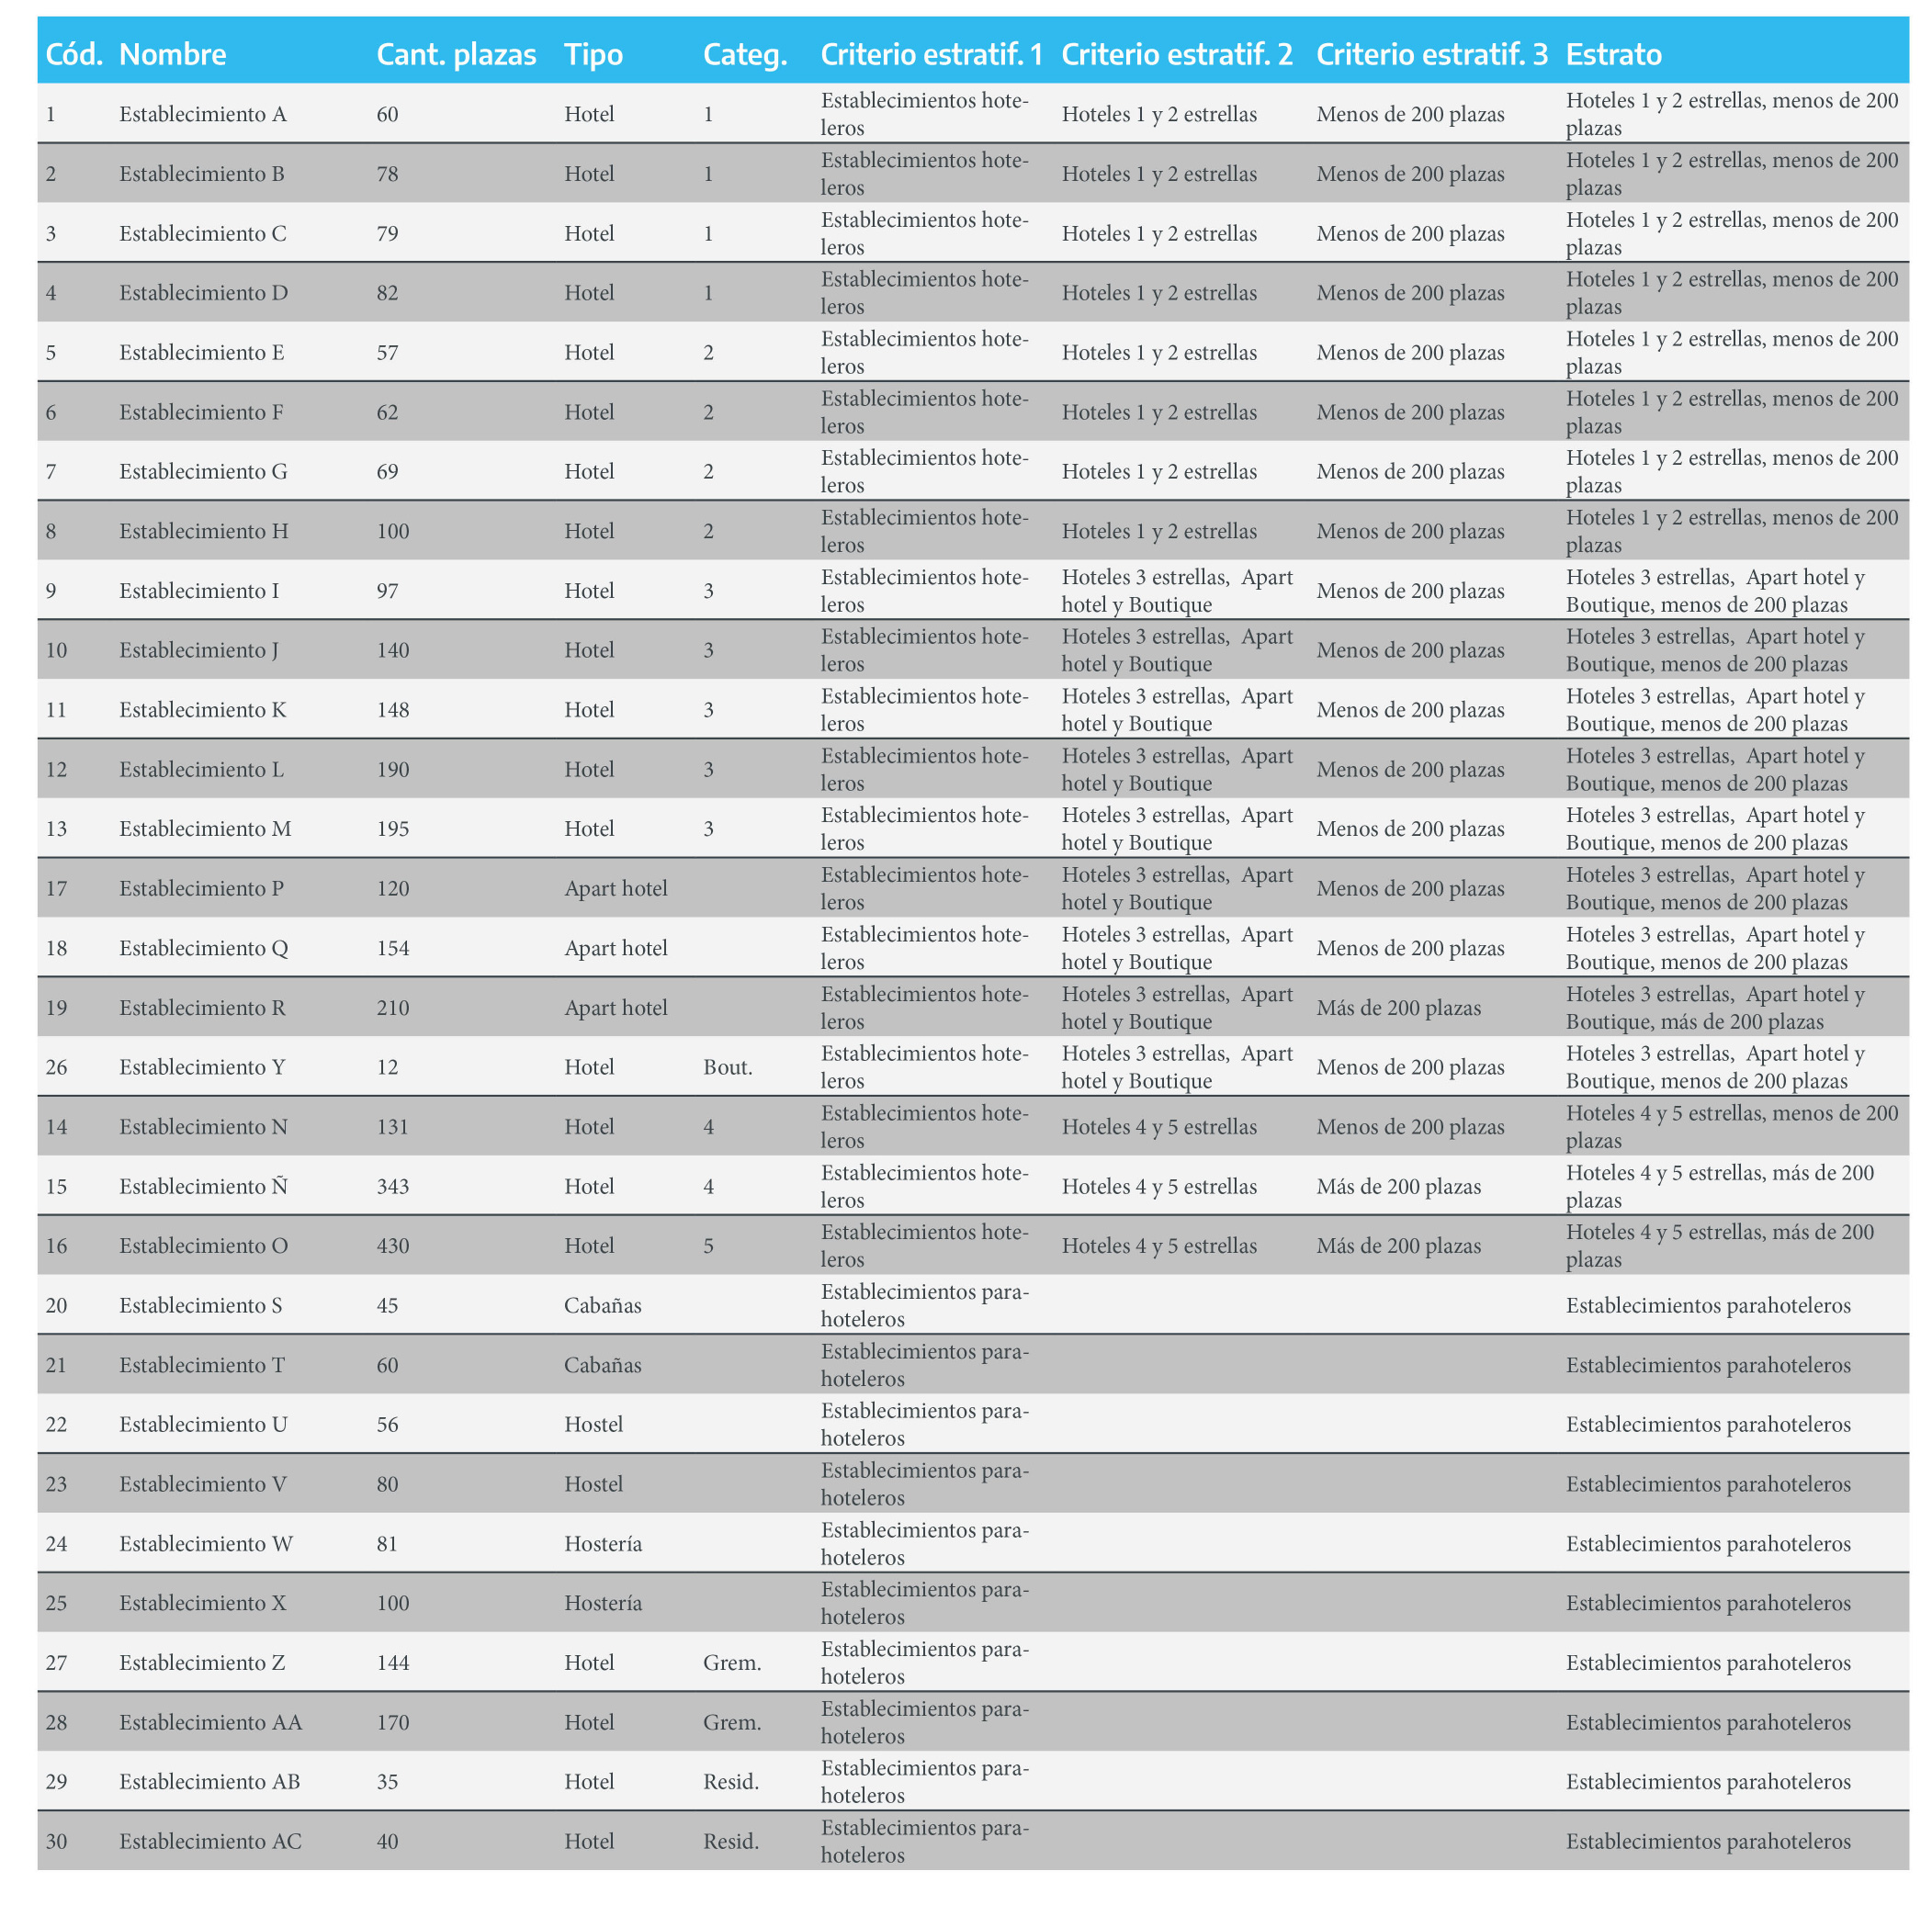
\includegraphics[width=1\linewidth]{imagenes/tabla_2} 

}

\caption{ Criterios de estratificación y definición de los estratos}\label{fig:criterios-estratos}
\end{figure}

\hypertarget{determinaciuxf3n-del-tamauxf1o-muestral-de-cada-estrato}{%
\paragraph{Determinación del tamaño muestral de cada estrato}\label{determinaciuxf3n-del-tamauxf1o-muestral-de-cada-estrato}}

Como se mencionó en párrafos anteriores, para determinar el tamaño de muestra de cada estrato, es preciso que previamente se haya determinado el tamaño de muestra total para la localidad (es decir, considerando a todos los estratos). En este ejemplo no se desarrollará el proceso de cálculo del tamaño total, sino que se asumirá como dato existente. En este caso, se considerará un tamaño de muestra total de 15 casos\footnote{Como puede apreciarse, el tamaño de muestra total es muy pequeño. En este ejemplo se define tal tamaño solo con fines ilustrativos, más aún considerando que el padrón solo consta de 30 establecimientos.}.

En primer lugar, se decide que los hoteles de 4 y 5 estrellas deben tener inclusión forzosa dentro de la muestra total, es decir se relevarán todos los establecimientos de estas categorías independientemente de su cantidad de plazas, debido al bajo peso relativo que presentan en el total de establecimientos y al comportamiento diferencial que tiene este segmento respecto al resto del universo. Por tanto, al total de 15 establecimientos de la muestra final se le deberán restar los 3 establecimientos que forman parte de los estratos ``Hoteles 4 y 5 estrellas, menos de 200 plazas'' y ``Hoteles 4 y 5 estrellas, más de 200 plazas'' , quedando un total de 12 establecimientos que deben ser distribuidos entre los restantes estratos.

Por otro lado, siguiendo el mismo razonamiento que en el caso previo, también se toma la decisión de que los establecimientos de 200 o más plazas deben tener inclusión forzosa en la muestra total. Por tanto, el establecimiento R, que dispone de 210 plazas, deberá necesariamente formar parte de la muestra. Los establecimientos Ñ y O ya fueron incluidos forzosamente por tener categoría 4 y 5 estrellas, respectivamente, por lo cual no es necesario repetir el proceso de selección. En esta instancia, quedan 11 establecimientos a ser repartidos entre los diferentes estratos.

El siguiente paso consiste en calcular el tamaño de las muestras de los siguientes estratos:

\begin{itemize}
\item
  Hoteles 1 y 2 estrellas, menos de 200 plazas.
\item
  Hoteles 3 estrellas, Apart hotel y Boutique, menos de 200 plazas.
\item
  Establecimientos parahoteleros.
\end{itemize}

El equipo técnico de la provincia X tomó la decisión de que la asignación de casos por estrato se ajuste al peso que cada uno tiene sobre el universo total de establecimientos, obviamente restando los alojamientos de 4 y 5 estrellas y el establecimiento de 210 plazas, perteneciente este último al estrato ``Hoteles 3 estrellas, Apart hotel y Boutique, más de 200 plazas'' . El peso de cada estrato se definirá en función de la cantidad de plazas disponibles del mismo, ya que ésta será una de las principales variables de análisis\footnote{Otra variable en función de la cual se pueden calcular los pesos de los estratos podría ser habitaciones disponibles, siempre y cuando las habitaciones sean la (o una de las) unidad/es de análisis.}. En el siguiente cuadro se realiza el cálculo del peso de cada estrato sobre el total de plazas, luego de haber sustraído las plazas correspondientes a los establecimientos previamente mencionados.

\begin{figure}

{\centering 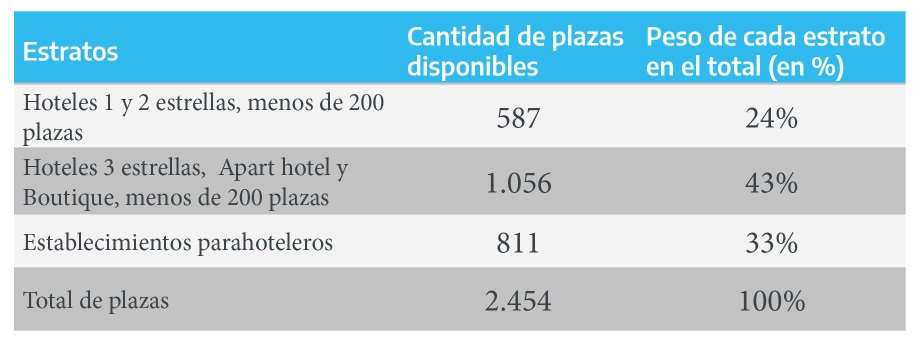
\includegraphics[width=1\linewidth]{imagenes/tabla_2A} 

}

\caption{Cantidad de plazas}\label{fig:cantidad-de-plazas}
\end{figure}

\begin{figure}

{\centering 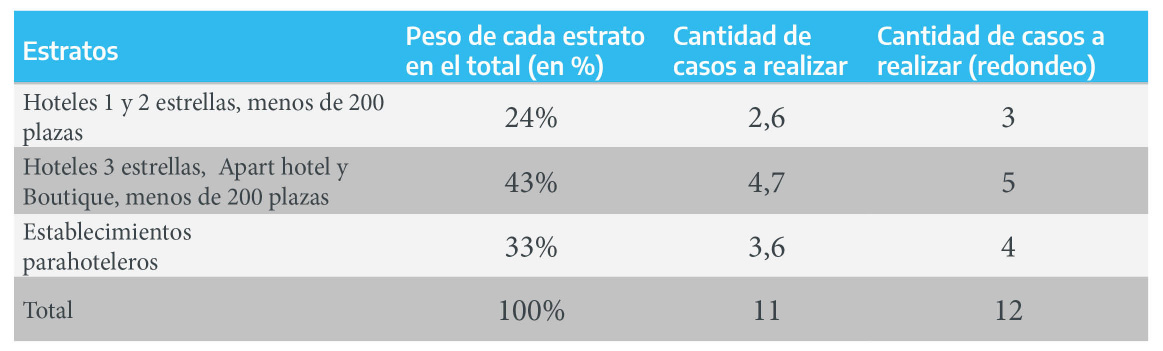
\includegraphics[width=1\linewidth]{imagenes/tabla_2B} 

}

\caption{Peso de estrato}\label{fig:peso-de-estrato}
\end{figure}

Los cálculos arrojan que habría que relevar 3 establecimientos del estrato ``Hoteles 1 y 2 estrellas, menos de 200 plazas'' , 5 del estrato ``Hoteles 3 estrellas, Apart hotel y Boutique, menos de 200 plazas y 4 del estrato''Establecimientos parahoteleros" , dando un total de 12 casos. Cabe mencionar que los redondeos suelen dar como resultado un leve aumento del tamaño de muestra originalmente planteado.

La muestra final de establecimientos quedaría distribuida de la siguiente forma:

\begin{figure}

{\centering 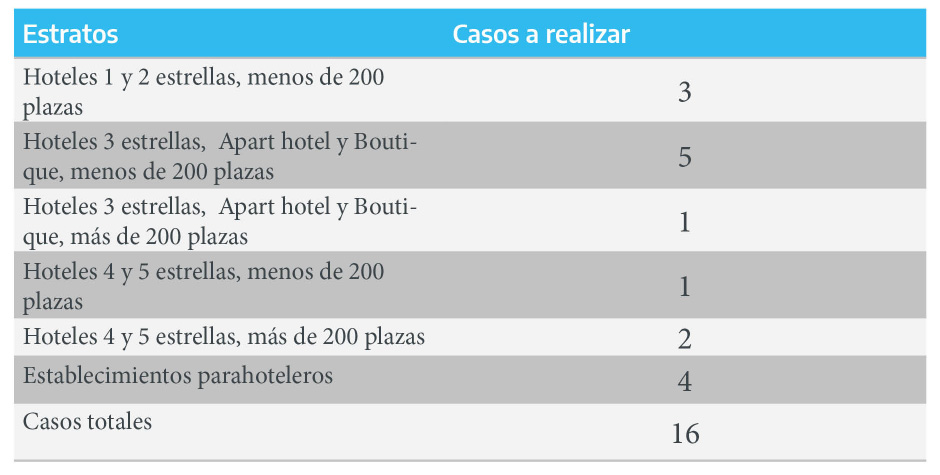
\includegraphics[width=1\linewidth]{imagenes/tabla_2C} 

}

\caption{Casos a realizar}\label{fig:casos-a-realizar}
\end{figure}

Una vez que determinados los tamaños de muestra de cada estrato, se procede con la selección de los casos.

\hypertarget{selecciuxf3n-de-los-casos-al-interior-de-cada-estrato}{%
\paragraph{Selección de los casos al interior de cada estrato}\label{selecciuxf3n-de-los-casos-al-interior-de-cada-estrato}}

Dentro de cada estrato, se ordenan los casos en función de la variable plazas disponibles, ya que se supone que tiene correlación con el comportamiento de las variables bajo estudio, siguiendo algún sentido (de menor a mayor, o viceversa). En este caso, se ordena de menor a mayor.

Luego se enumeran los establecimientos dentro de cada estrato.

Seguidamente se calcula el ``intervalo de selección'' , que es el resultado de dividir la cantidad de establecimientos total del estrato (Nf) por el tamaño de la muestra en el mismo (nf). Como ya se mencionó previamente, el intervalo de selección define la cantidad de establecimientos que debe haber entre una y otra selección. De este modo, el intervalo de selección en cada estrato será:

\begin{itemize}
\item
  Hoteles 1 y 2 estrellas, menos de 200 plazas: \(8/3\)=\(2,7\)=\(3\)\textbf{.}
\item
  Hoteles 3 estrellas, Apart hotel y Boutique, menos de 200 plazas: \(8/5\)=\(1,6\)=\(2\)\textbf{.}
\item
  Establecimientos parahoteleros: \(10/4\)=\(2,5\)=\(3\)\textbf{.}
\end{itemize}

El paso siguiente es, dentro de cada estrato, elegir aleatoriamente un número (r) entre 1 y el resultado de N/n.~Este número definirá la posición del establecimiento a partir del cual comienza la selección sistemática (arranque aleatorio). Supóngase que los números aleatorios obtenidos para cada estrato son:

\begin{itemize}
\item
  Hoteles 1 y 2 estrellas, menos de 200 plazas: \(r=2\).
\item
  Hoteles 3 estrellas, Apart hotel y Boutique, menos de 200 plazas: \(r=2\).
\item
  Establecimientos parahoteleros: \(r=1\).
\end{itemize}

En esta instancia se está en condiciones de realizar la selección sistemática de los establecimientos a ser relevados, tal como se muestra a continuación.

\begin{figure}

{\centering 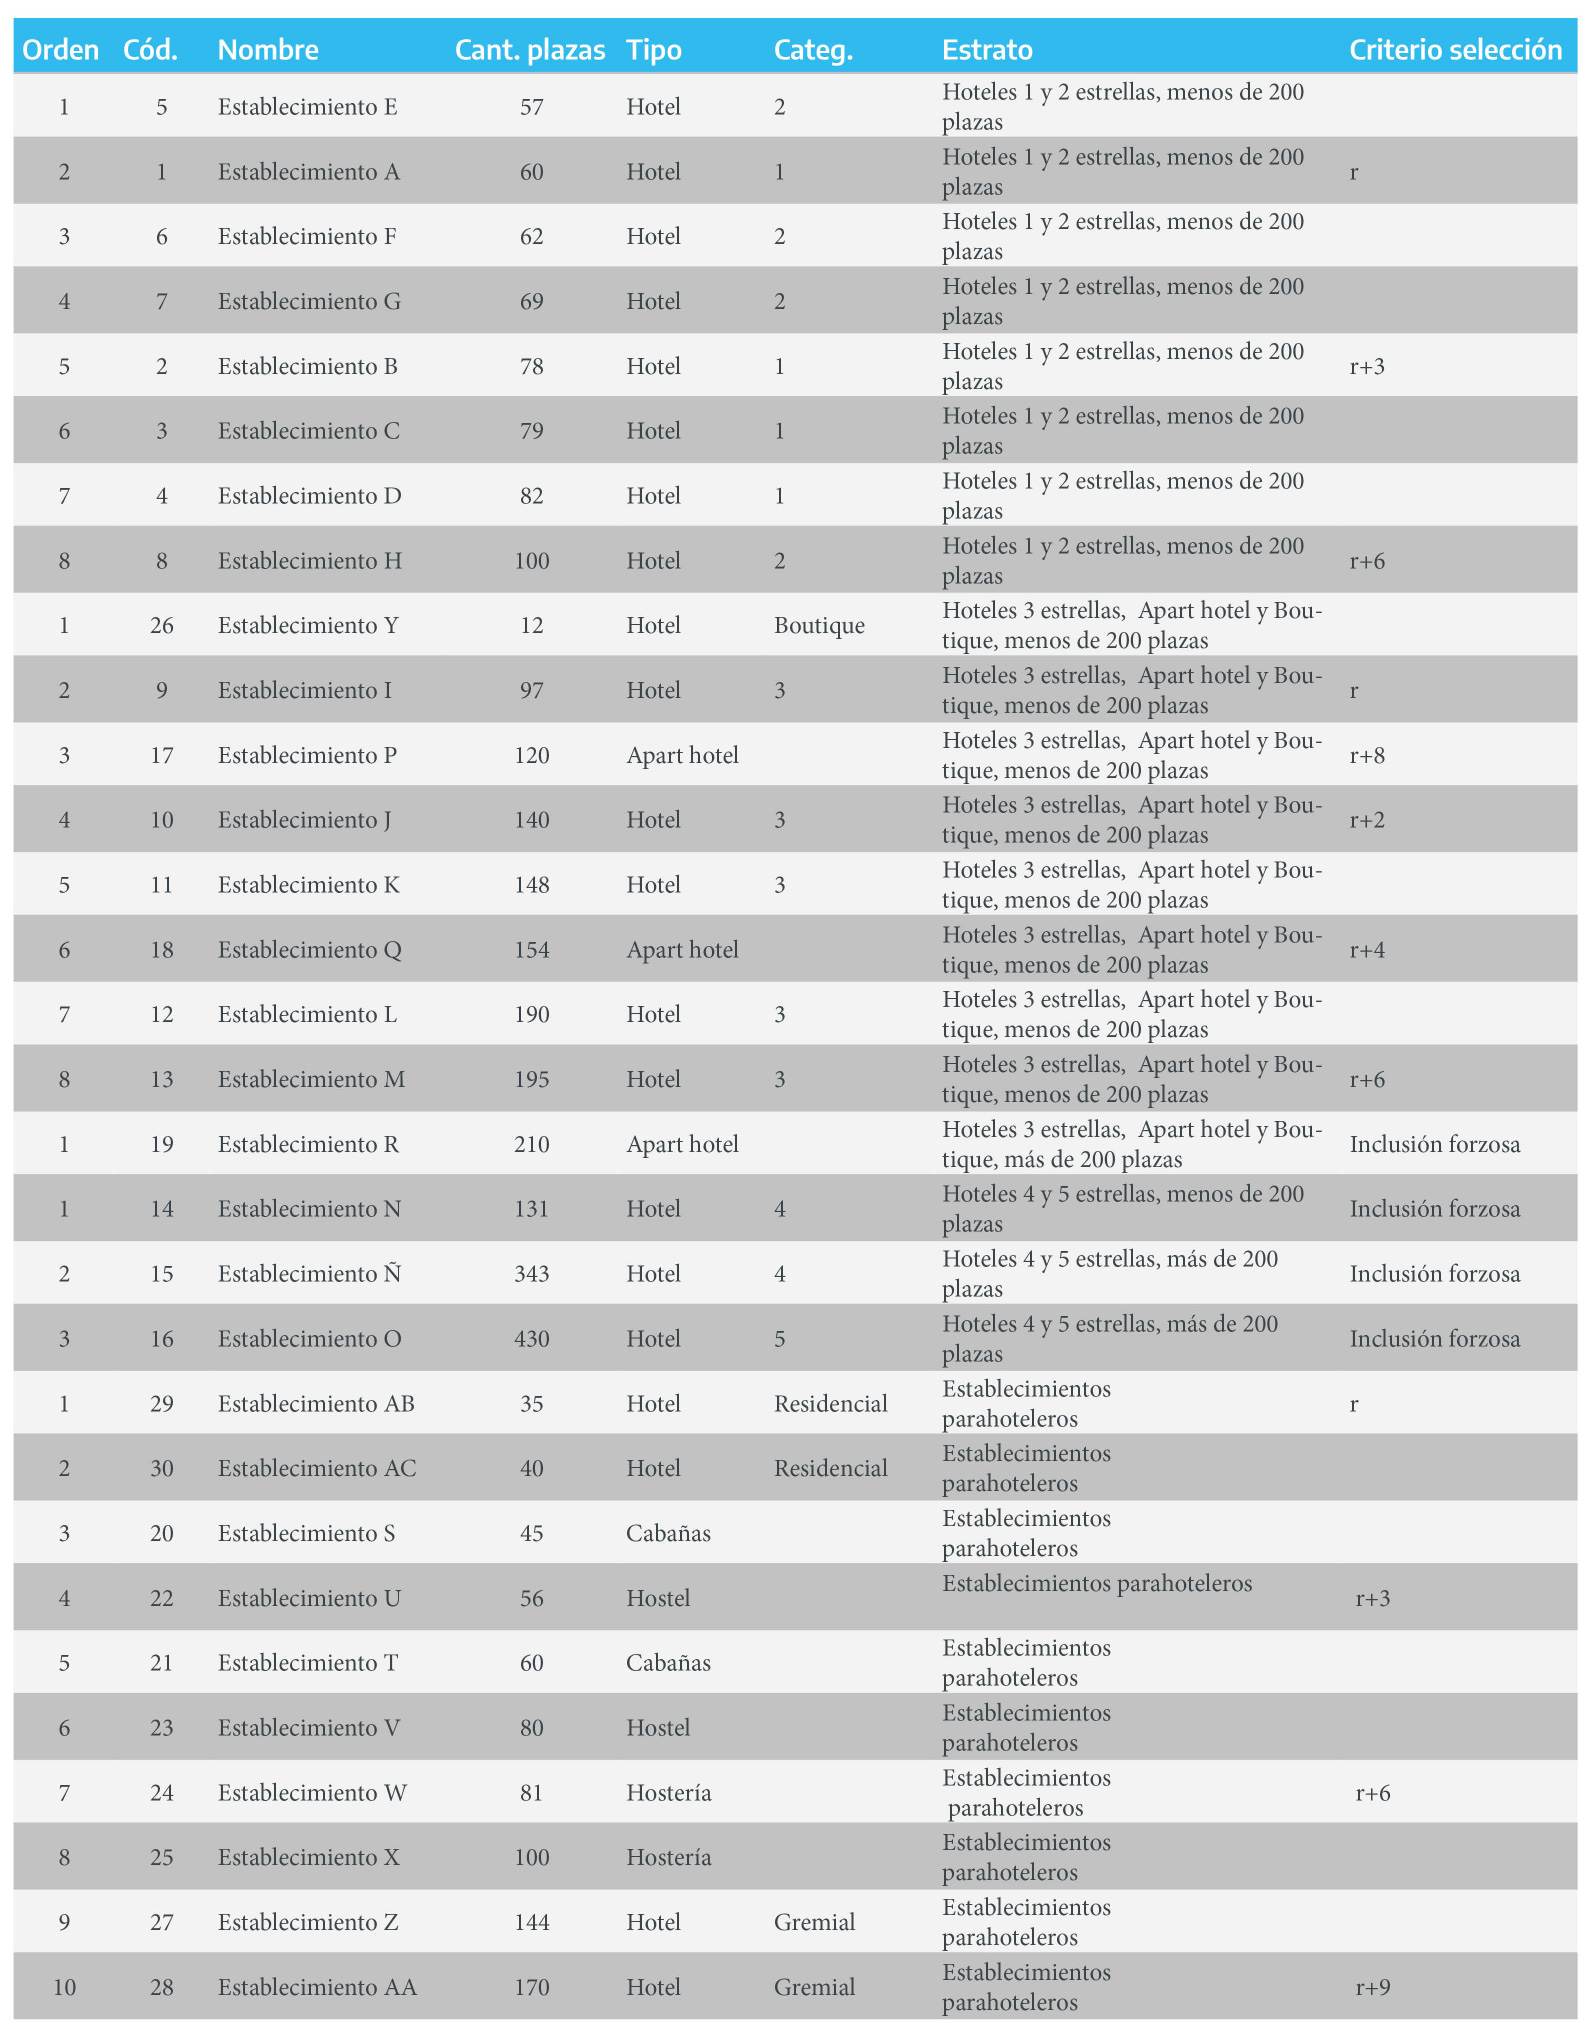
\includegraphics[width=1\linewidth]{imagenes/tabla_3} 

}

\caption{Selección de las muestras al interior de cada estrato}\label{fig:muestra-interior}
\end{figure}

Nótese que, en cada estrato, el primer elemento seleccionado es el definido por el arranque aleatorio (r). Luego, el segundo elemento estará definido por \(r\)+(\(N/n\)=intervalo de selección). Por ejemplo, en el estrato ``Hoteles 1 y 2 estrellas, menos de 200 plazas'' , el segundo elemento será el que está ubicado en la posición 5, ya que \(2+3\)=\(5\); y el tercer elemento será \(2+6\)=\(8\).

En el estrato ``Hoteles 3 estrellas, Apart hotel y Boutique, menos de 200 plazas'' , el último establecimiento seleccionado es el que se encuentra en la posición 3, ya que el inmediatamente anterior fue el 8, y luego de esta posición ya no había más establecimientos, por lo cual fue necesario realizar la selección desde el principio.

Finalmente, los establecimientos que componen la muestra son:

\begin{figure}

{\centering 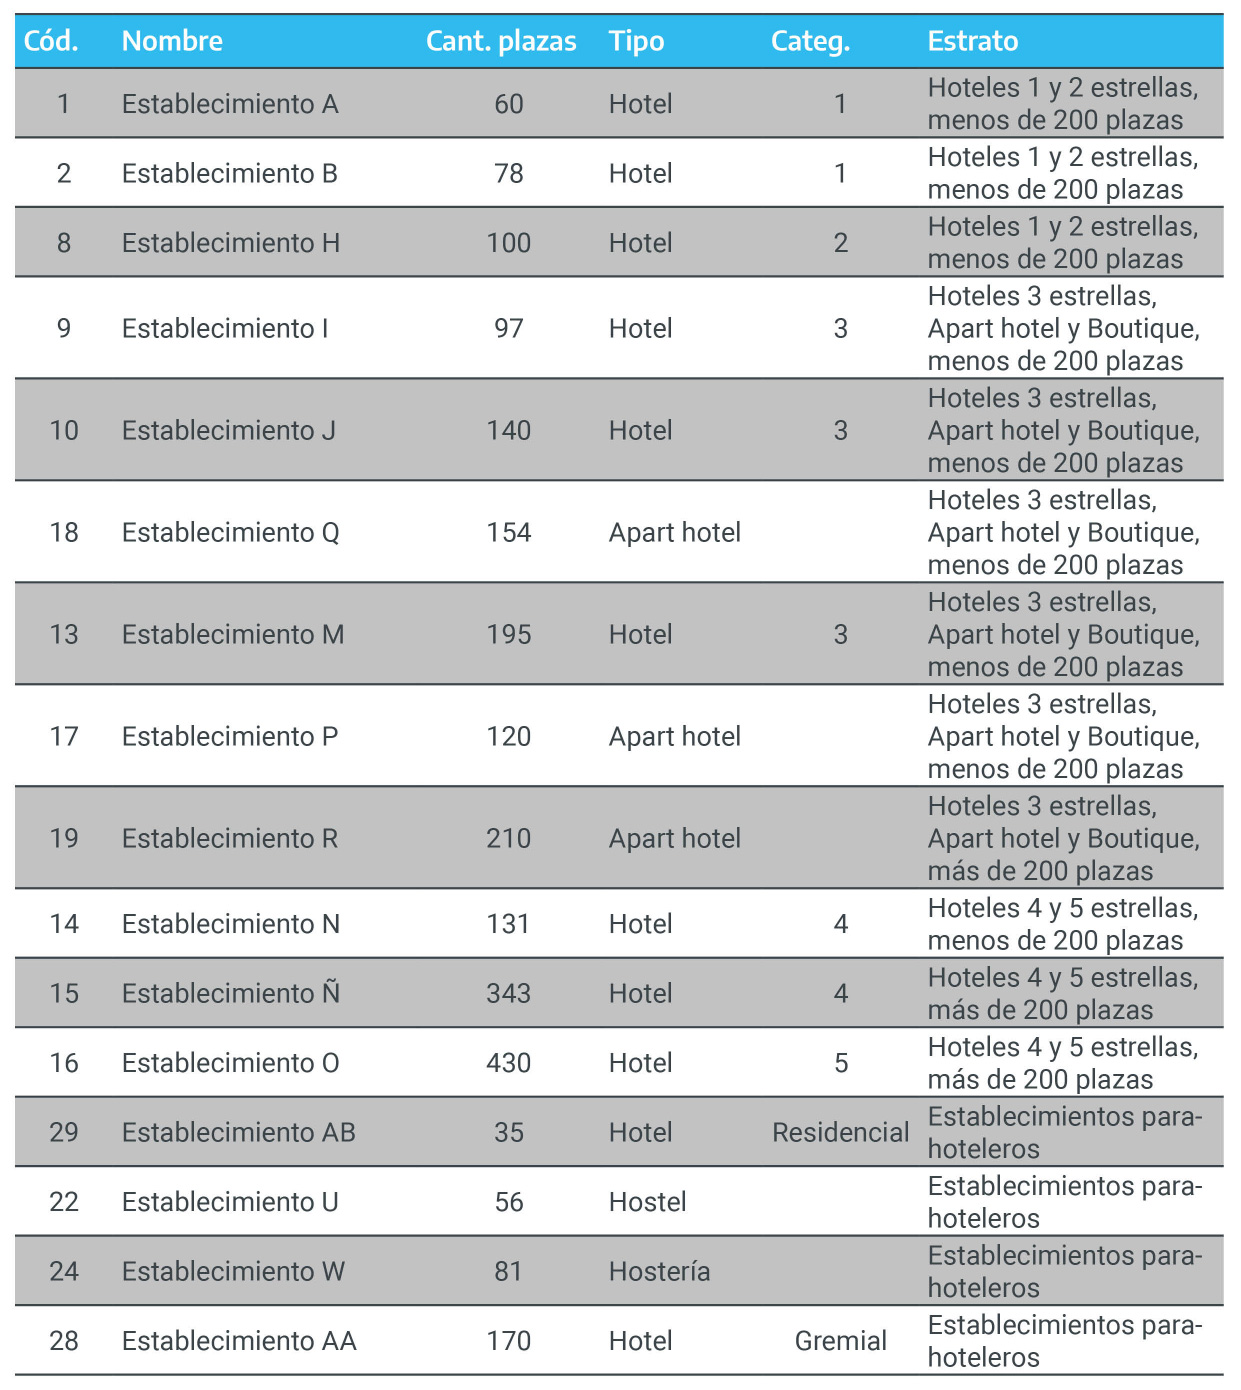
\includegraphics[width=1\linewidth]{imagenes/tabla_4} 

}

\caption{Muestra final de establecimientos}\label{fig:muestra-final}
\end{figure}

Por último, recuérdese que los criterios elegidos en este ejemplo para la estratificación son hipotéticos. Por tanto, en cada provincia y/o municipio, los criterios a partir de los cuales se estratificará al universo de establecimientos dependerán de la realidad propia del sector así como a los objetivos de estudio.

\hypertarget{construcciuxf3n-del-formulario-de-registro-cuestionario-o-planilla-definiciuxf3n-de-variables-fundamentales}{%
\subsection{Construcción del formulario de registro (cuestionario o planilla): definición de variables fundamentales}\label{construcciuxf3n-del-formulario-de-registro-cuestionario-o-planilla-definiciuxf3n-de-variables-fundamentales}}

Un aspecto central en el diseño de una investigación es la definición de las \textbf{variables}, que son las características o atributos que interesan ser observados o medidos en la población bajo estudio. Por ejemplo, en el caso específico de los relevamientos de alojamientos turísticos, las variables específicas a medir pueden ser ``cantidad de plazas ocupadas'' , ``cantidad de plazas disponibles'' , ``cantidad de habitaciones ocupadas'' , ``cantidad de habitaciones disponibles'' , ``nuevos viajeros alojados'' , ``tarifa media'' , etc. Lógicamente, las variables se desprenden de los objetivos de investigación. Por lo tanto, cuánto más claros sean los objetivos, mayor será la probabilidad de plantear variables relevantes que permitan alcanzarlos.

En las investigaciones de carácter socio-económico, dentro de las cuales se incluyen los relevamientos de alojamientos turísticos, la información referida a las variables de estudio es recolectada por medio de \textbf{preguntas}, que suelen estar dispuestas en \textbf{cuestionarios}. El cuestionario es, por lo tanto, el instrumento de recolección de información sobre variables que buscan caracterizar a una población\footnote{Los operativos de algunas provincias/departamentos/municipios, en lugar de emplear cuestionarios en sentido estricto, utilizan planillas, en cuyas filas están registrados los establecimientos a ser relevados y en donde las variables o preguntas están dispuestas en las columnas. Las planillas suelen ser digitales (en Excel o Access) o en papel. Una de las ventajas de las planillas digitales es que permiten omitir el paso de ``carga de datos'' . Este formato de instrumento de medición suele ser utilizado en los relevamientos telefónicos.}.

Las variables pueden ser medidas de forma directa o indirecta. Las variables de medición directa son aquellas que pueden ser obtenidas mediante una sola pregunta. Por ejemplo, el valor de la variable plazas ocupadas se obtiene mediante la pregunta: ¿cuál es la cantidad de plazas ocupadas? Por otro lado, existen variables que presentan un mayor grado de abstracción o complejidad, y que requieren de más de una pregunta para ser medidas. Este es el caso de, por ejemplo, la tasa o porcentaje de ocupación en plazas, que se obtiene mediante el cociente entre cantidad de plazas ocupadas y cantidad de plazas disponibles (es decir, dos variables distintas).

Para finalizar, en este documento se asimilará el concepto de variable con el de indicador, a pesar de que ambos puedan presentar diferencias sutiles. En este sentido, plazas ocupadas y tasa de ocupación en plazas, así como otras variables referidas a alojamientos turísticos, constituyen indicadores.

\hypertarget{variables-e-indicadores-en-una-encuesta-de-alojamientos-turuxedsticos}{%
\subsubsection{Variables e indicadores en una encuesta de alojamientos turísticos}\label{variables-e-indicadores-en-una-encuesta-de-alojamientos-turuxedsticos}}

En este sub-apartado se presentarán las diferentes variables que pueden ser relevadas a través de una encuesta de alojamientos turísticos. En primer lugar se enumeran y describen aquellas variables cruciales para la estimación de indicadores básicos, tales como porcentaje de ocupación en plazas y/o habitaciones, o pernoctaciones.

Por tanto, las variables elementales que pueden ser relevadas en este tipo de operativos son:

\begin{itemize}
\item
  plazas ocupadas;
\item
  plazas disponibles;
\item
  habitaciones o unidades ocupadas\footnote{En establecimientos no hoteleros como complejos de cabañas, apart hoteles, complejos de departamentos y campings, ya no se mide la ocupación y disponibilidad en habitaciones, sino en la misma unidad. En los complejos de cabañas, la unidad es la misma cabaña; en los apart hoteles y complejos de departamentos, el departamento; en los campings, la parcela.};
\item
  habitaciones o unidades disponibles;
\item
  cantidad de nuevos viajeros alojados (o cantidad de viajeros ingresados);
\item
  (eventualmente) lugar de residencia de los viajeros alojados.
\end{itemize}

La variable \textbf{``plazas ocupadas''} resulta crucial, dado que constituye uno de los insumos elementales para la estimación del \textbf{``porcentaje de ocupación en plazas''} (plazas ocupadas / plazas disponibles, en un período determinado) y de las \textbf{``pernoctaciones''} (suma de las plazas ocupadas de todos los establecimientos en un período determinado). En el caso del porcentaje de ocupación en plazas, como se observa, la variable plazas ocupadas interviene en el numerador de la fórmula de cálculo.

Es recomendable que, la cantidad de plazas ocupadas sea relevada en términos absolutos (es decir, como cantidad). El mismo criterio aplica para la \textbf{cantidad de habitaciones ocupadas}, variable que participa en la estimación del porcentaje de ocupación en habitaciones (cuya fórmula es cantidad de habitaciones ocupadas/ cantidad de habitaciones disponibles).

En este sentido, muchas jurisdicciones suelen preguntar directamente por el porcentaje de ocupación correspondiente en ese lugar durante un periodo dado. Luego, multiplican ese porcentaje por la cantidad de plazas o habitaciones disponibles (según corresponda), obteniendo de ese modo los valores absolutos. Esta forma de cálculo encierra muy probablemente un tipo de error no estadístico, que es de una magnitud mayor a cuando se pregunta por cantidades y, complicando aún más la situación, esa cuantía no puede ser estimada. El error está en suponer que el informante responderá en forma precisa por la tasa de ocupación, cuando es posible que su subjetividad lo sesgue a declarar un valor ``promedio'' (perdiendo sentido la serie histórica que el estudio procura construir) o bien de algún sub-período del periodo de referencia (un fin de semana, en lugar de toda la semana por ejemplo). Asimismo, el entrevistado también puede confundir el porcentaje de ocupación en plazas con el porcentaje de ocupación en habitaciones. Cuánto más concreta y objetiva sea la pregunta, mayor será la calidad de la información obtenida.

Adicionalmente, es conveniente también indagar siempre por la cantidad de "\textbf{plazas disponibles"} y \textbf{``habitaciones disponibles''}, variables que formarán parte del denominador en las estimaciones de \textbf{``porcentaje de ocupación en plazas''} y \textbf{``porcentaje de ocupación en habitaciones''}, respectivamente. Si bien la información referida a disponibilidad en plazas y habitaciones puede estar presente en el padrón de establecimientos de alojamiento turístico, la medición de estas variables en el relevamiento podría ser útil, con el doble propósito de:

\begin{itemize}
\item
  contar con información actualizada al momento de realizar las estimaciones: las plazas y habitaciones disponibles del período analizado puede diferir respecto a la del padrón, debido a cierres temporarios o definitivos de establecimientos, o clausura temporaria o definitiva de habitaciones (con la consecuente reducción de plazas);
\item
  corregir posibles inconsistencias o actualizar la información del padrón de alojamientos (cuando corresponda);
\end{itemize}

La variable \textbf{``cantidad de nuevos viajeros alojados (o cantidad de viajeros ingresados)''} también resulta útil para realizar una aproximación a la estimación de la cantidad de turistas en el destino. Si se decide medirla, es preciso que se clarifique que lo correcto es registrar la cantidad de \textbf{nuevos} viajeros en el período de referencia, y no la cantidad de total viajeros alojados. En efecto, en este último caso, se estaría contando más de una vez al mismo viajero. Si por algún motivo no se pudiese incluir esta pregunta, es posible realizar una estimación de la cantidad de viajeros dividiendo pernoctaciones en determinado período por ``estadía promedio'' . La información sobre estadía promedio es conveniente obtenerla de otra fuente de información (por ejemplo, encuestas de demanda o perfil del turista), dado que al indagar directamente por la estadía promedio se correría el riesgo de caer en posibles errores de cálculo por parte del respondente (además de mediar su subjetividad).

En caso de incorporarse a la medición la variable \textbf{``lugar de residencia habitual'' ,} debajo se propone una clasificación posible, con un nivel de desagregación de máxima, que cada jurisdicción acotará (o no) atendiendo a los objetivos propios de investigación y a la duración del cuestionario.

\begin{figure}

{\centering 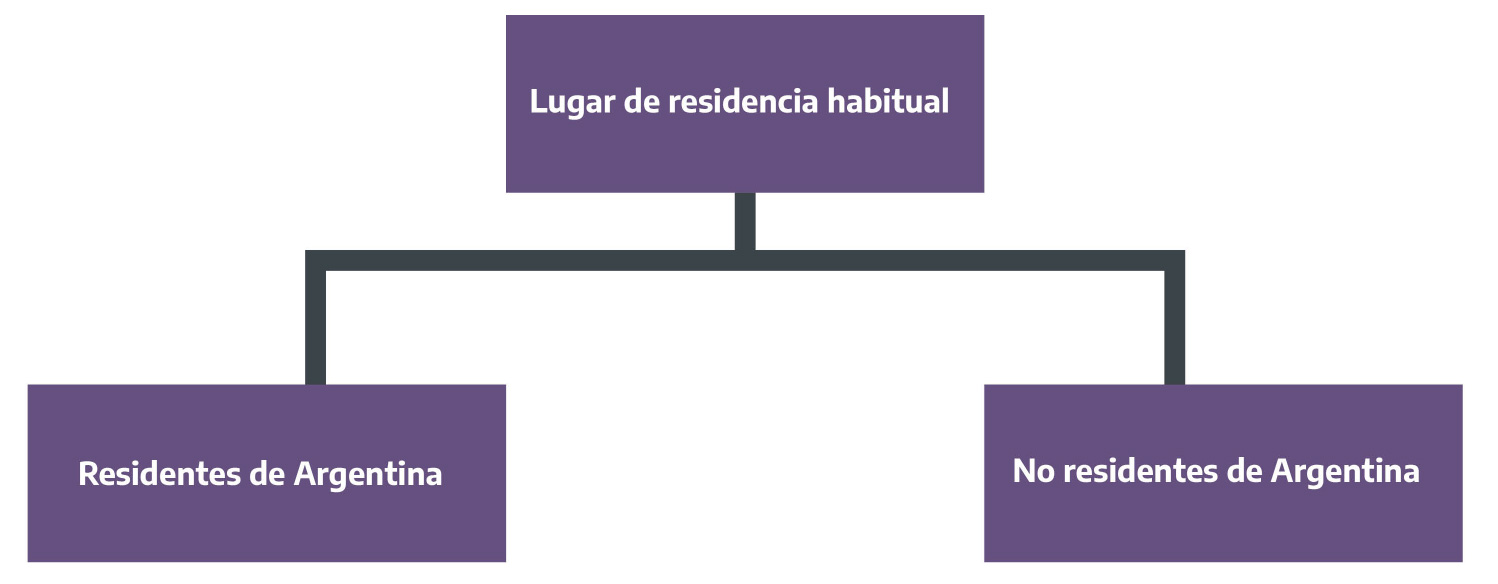
\includegraphics[width=1\linewidth]{imagenes/figura_2} 

}

\caption{Lugar de residencia habitual}\label{fig:residencia-habitual}
\end{figure}

\begin{figure}

{\centering 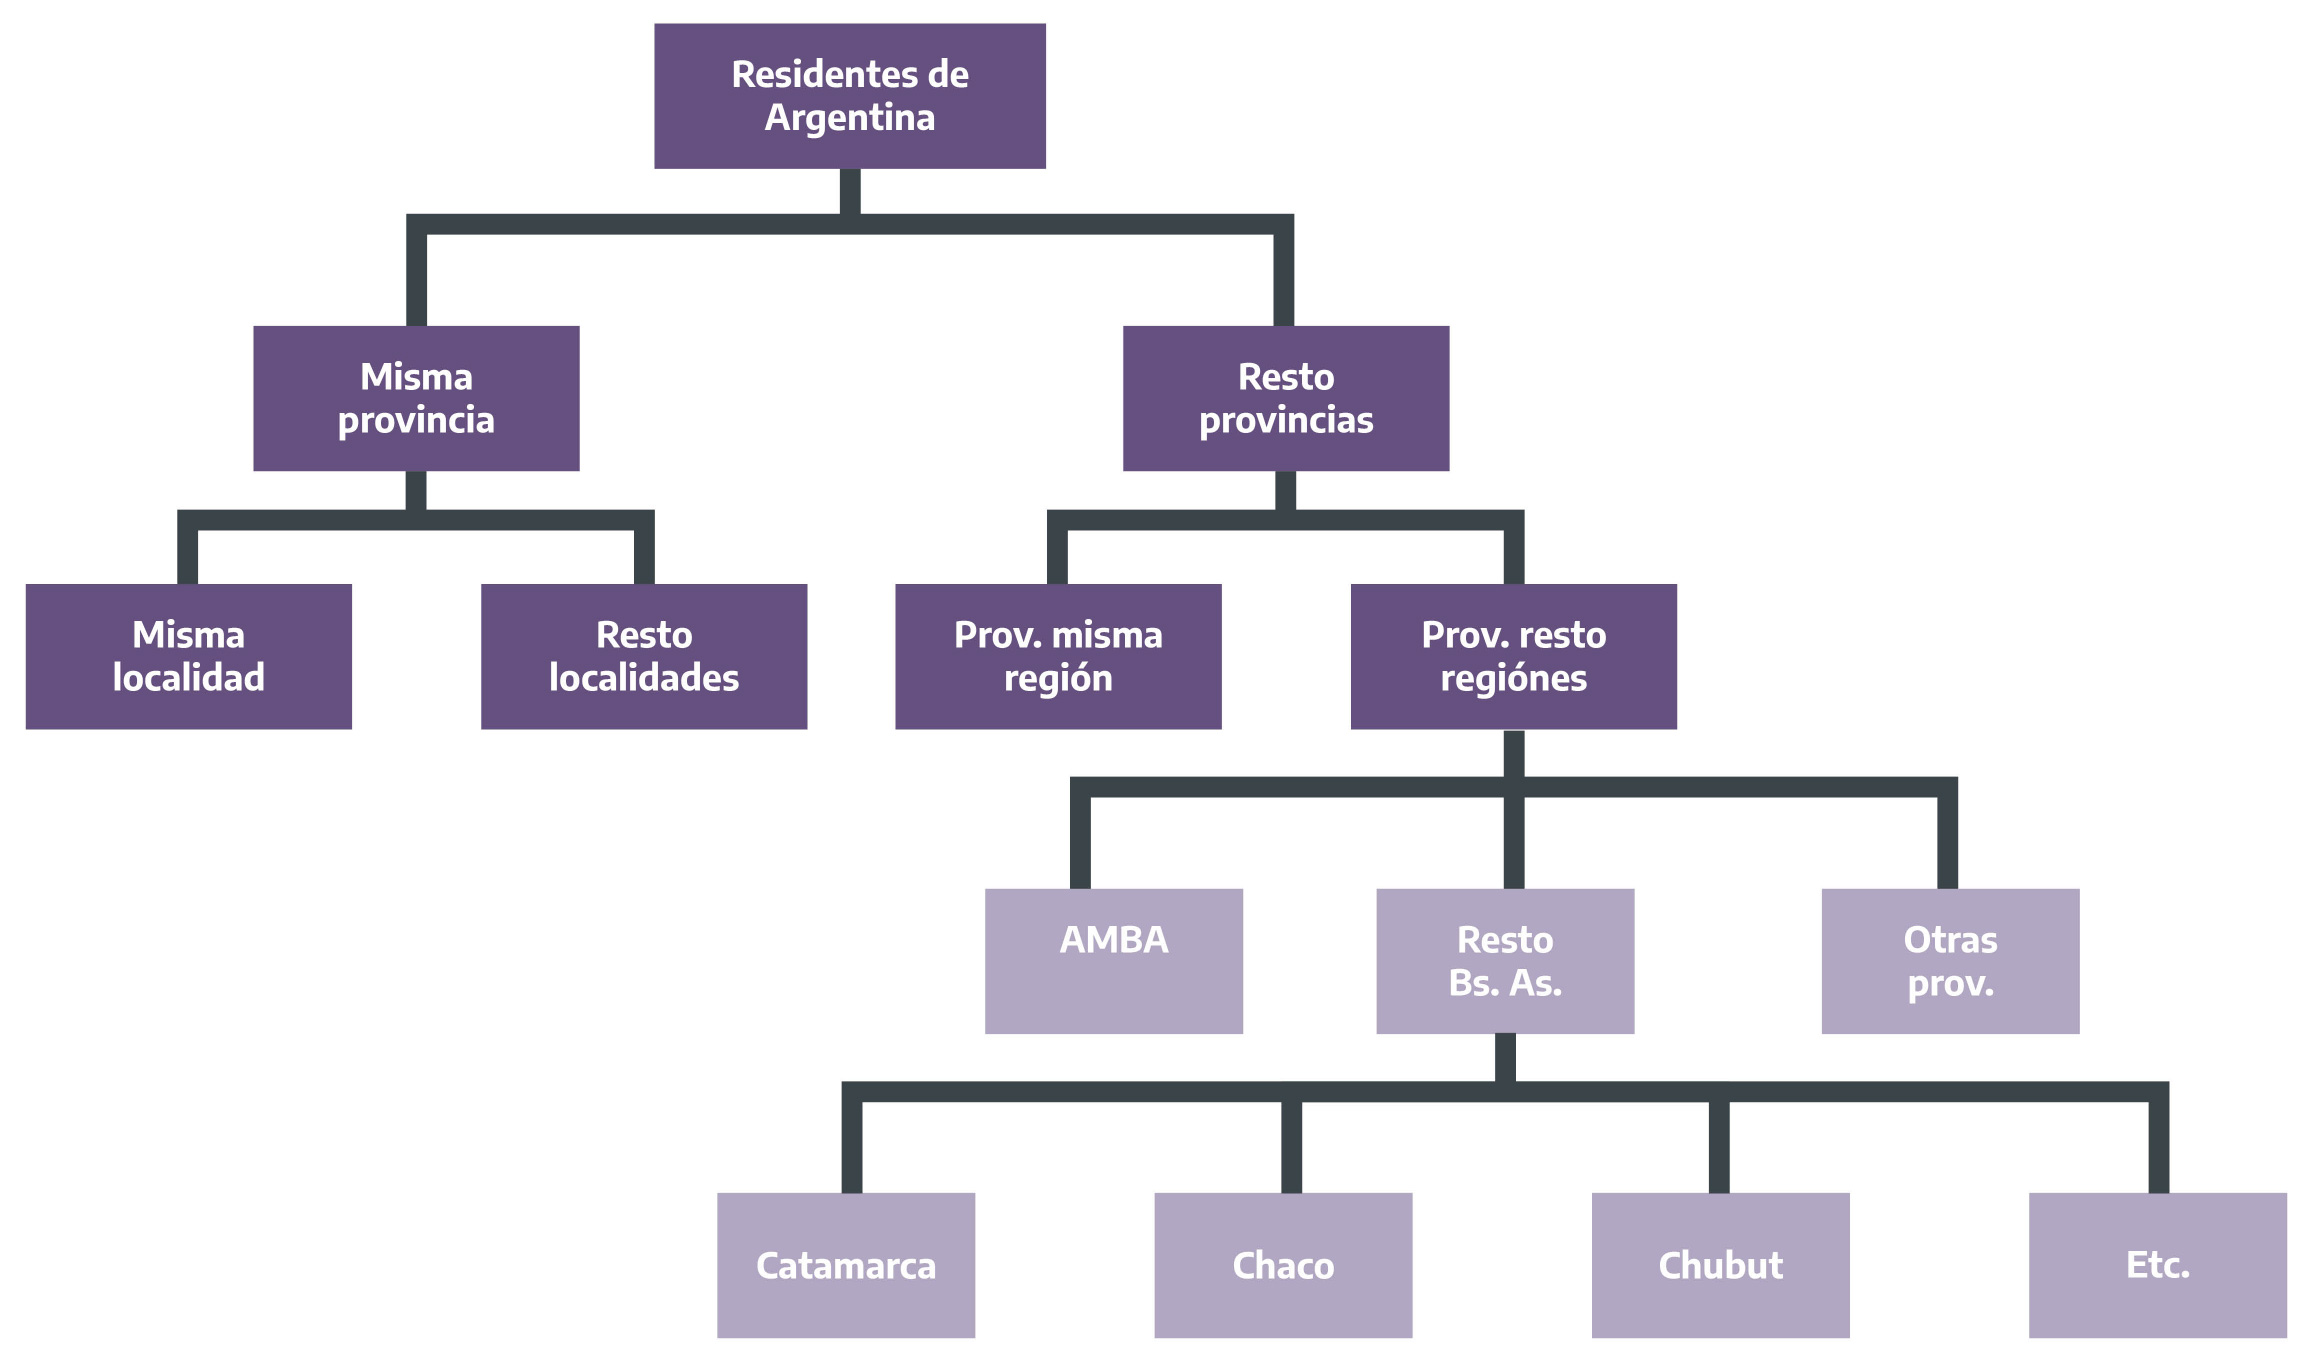
\includegraphics[width=1\linewidth]{imagenes/figura_2_1} 

}

\caption{Lugar de residencia habitual. Residentes de Argentina}\label{fig:residentes}
\end{figure}

\hfill\break

\begin{figure}

{\centering 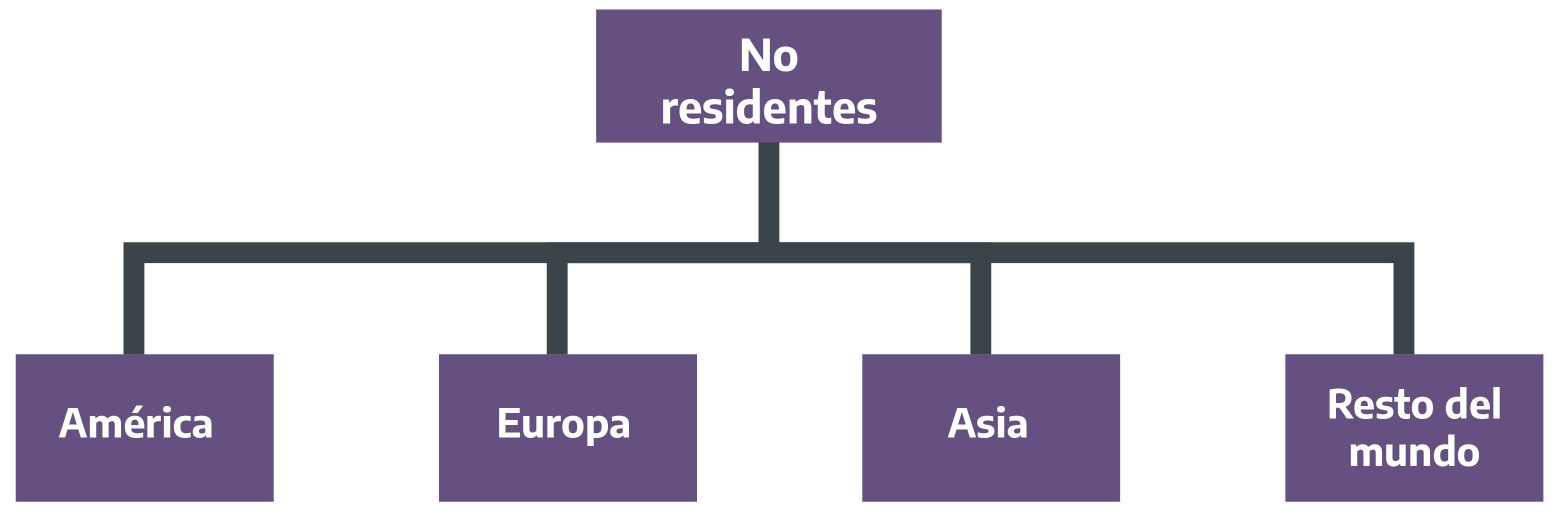
\includegraphics[width=1\linewidth]{imagenes/figura_2_2} 

}

\caption{Lugar de residencia habitual. No residentes de Argentina}\label{fig:no-residentes}
\end{figure}

\begin{figure}

{\centering 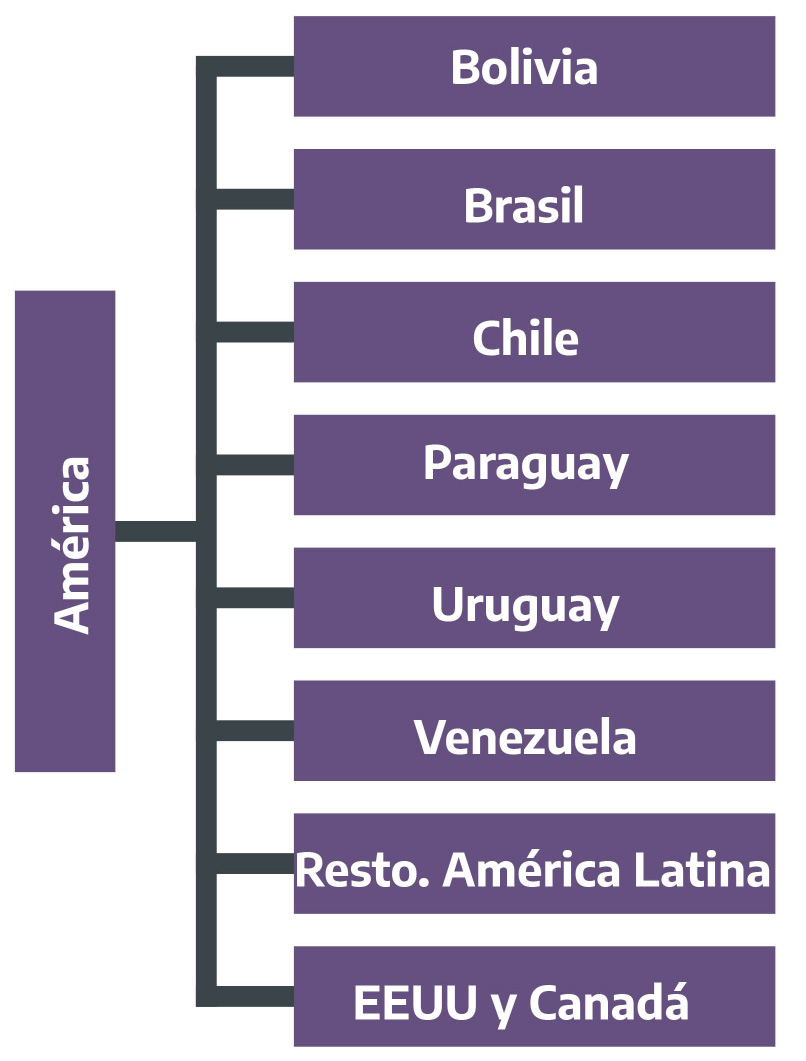
\includegraphics[width=1\linewidth]{imagenes/figura_2_2_1} 

}

\caption{Lugar de residencia habitual. No residentes de Argentina. América}\label{fig:america-latina}
\end{figure}

\begin{figure}

{\centering 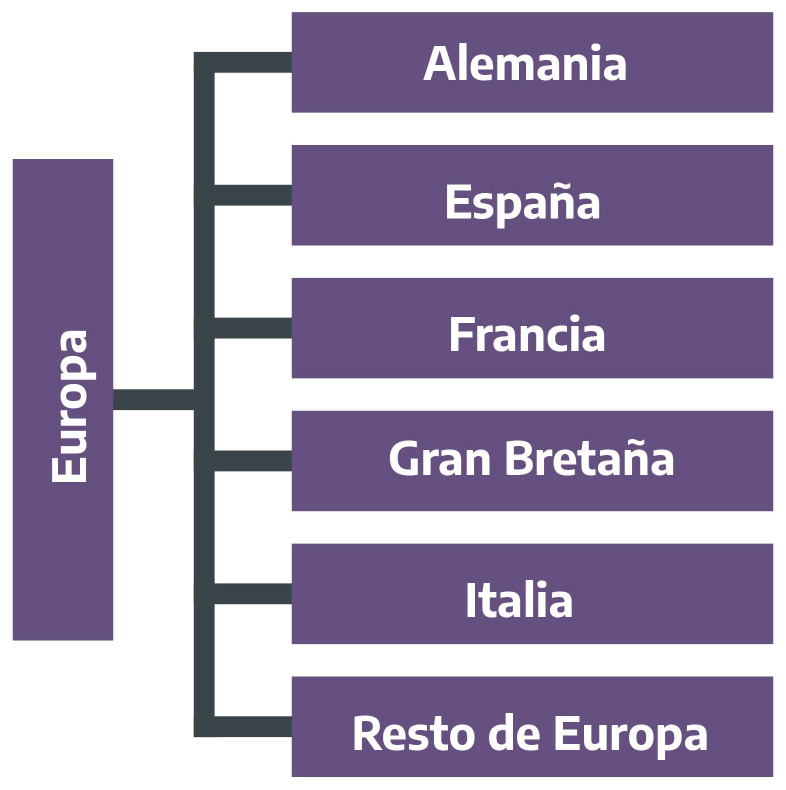
\includegraphics[width=1\linewidth]{imagenes/figura_2_2_2} 

}

\caption{Lugar de residencia habitual. No residentes de Argentina. Europa}\label{fig:europa}
\end{figure}

La medición de las variables mencionadas previamente resulta de gran importancia, dado que permiten estimar los diferentes indicadores que son objeto de estudio en las distintas provincias, departamentos y municipios del país. Sin embargo, si fuese necesario aplicar un cuestionario de menor duración, sería posible reducir la cantidad de variables a relevar. En cualquier caso, la variable fundamental, que no debería faltar en ningún relevamiento de alojamientos turísticos es ``plazas ocupadas'' , dado que, como ya se indicó, permite la estimación de otros indicadores fundamentales: porcentaje de ocupación en plazas y pernoctaciones. Luego de garantizar la inclusión de esta variable en el cuestionario (o planilla de registro), el orden recomendado de inclusión de otras variables sería ``plazas disponibles'' , ``habitaciones ocupadas'' , ``habitaciones disponibles'' y ``cantidad de nuevos viajeros alojados (o cantidad de viajeros ingresados)'' .

Como se desprende de lo desarrollado previamente, en caso de no incluir en el cuestionario a las variables ``plazas disponibles'' y ``habitaciones disponibles'' , la información sobre las mismas puede ser obtenida de los padrones de establecimientos de alojamiento turístico, tomando los recaudos necesarios en cuanto a su actualización.

Para finalizar, existen otras variables que pueden ser relevadas mediante un operativo de alojamientos:

\begin{itemize}
\tightlist
\item
  En relación al \textbf{empleo}, puede indagarse la cantidad de personas ocupadas en el establecimiento. Más aún, a las personas ocupadas se las podría clasificar tal como se sugiere debajo:
\end{itemize}

\begin{figure}

{\centering 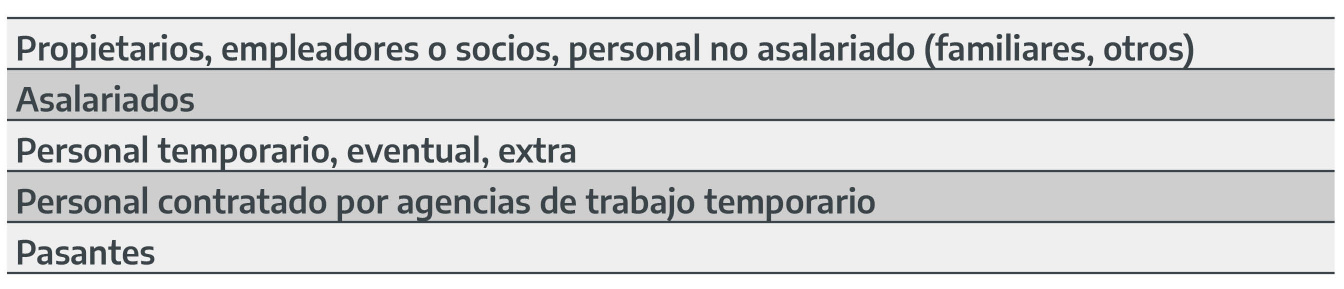
\includegraphics[width=1\linewidth]{imagenes/tabla_5} 

}

\caption{Categorías ocupacionales utilizadas en la EOH (MINTURDEP-INDEC)}\label{fig:ocupados}
\end{figure}

\textbf{Tarifas} en el período de referencia: las tarifas pueden ser medidas siguiendo diferentes criterios. Por ejemplo, pueden relevarse las tarifas de todos los tipos (single, doble, triple, cuádruple) y categorías (estándar, superior, etc.) de habitaciones del establecimiento. También puede indagarse la tarifa promedio del tipo de habitación con mayor cantidad de unidades disponibles en el establecimiento. Otra alternativa podría ser recabar la tarifa del tipo de habitación con mayor nivel de demanda. De forma similar a la anterior variable, cada jurisdicción podrá optar por el criterio de medición más adecuado a sus objetivos de estudio y características del relevamiento.\\

\hypertarget{clasificaciuxf3n-de-los-establecimientos-de-alojamiento-turuxedstico}{%
\section{Clasificación de los establecimientos de alojamiento turístico}\label{clasificaciuxf3n-de-los-establecimientos-de-alojamiento-turuxedstico}}

Sin perder de vista las particularidades provinciales/departamentales/municipales que encierra la definición de cada clase de establecimiento, producto de las normativas vigentes en cada jurisdicción, en este apartado se planteará una propuesta mínima de clasificación de los mismos. La misma es empleada en los padrones del MINTURDEP y puede ser útil para establecer equivalencias entre las diferentes definiciones adoptadas en cada jurisdicción.

\begin{figure}

{\centering 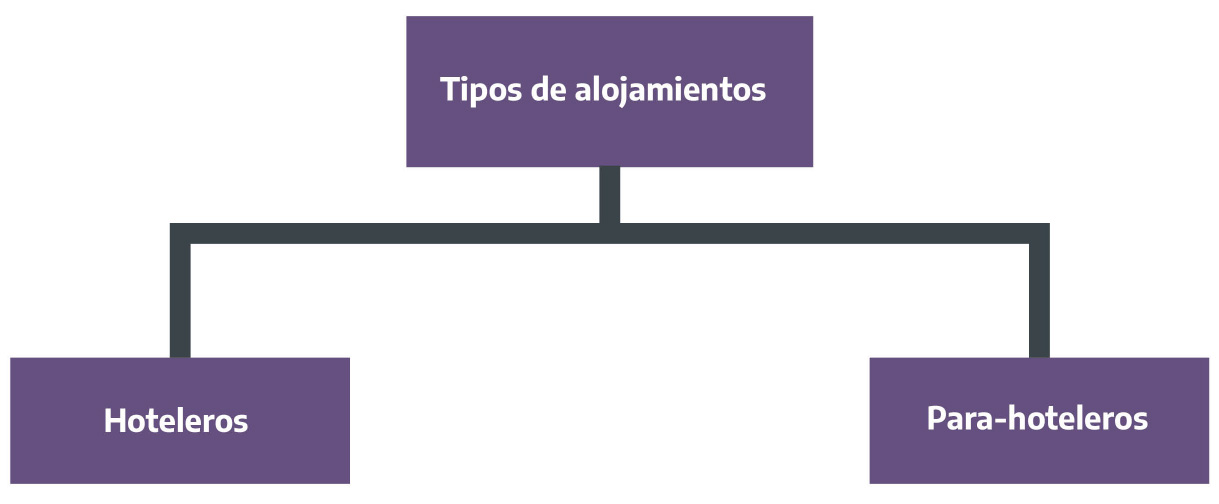
\includegraphics[width=1\linewidth]{imagenes/figura_3} 

}

\caption{Tipos de alojamientos turísticos}\label{fig:tipos-alojamientos}
\end{figure}

\begin{figure}

{\centering 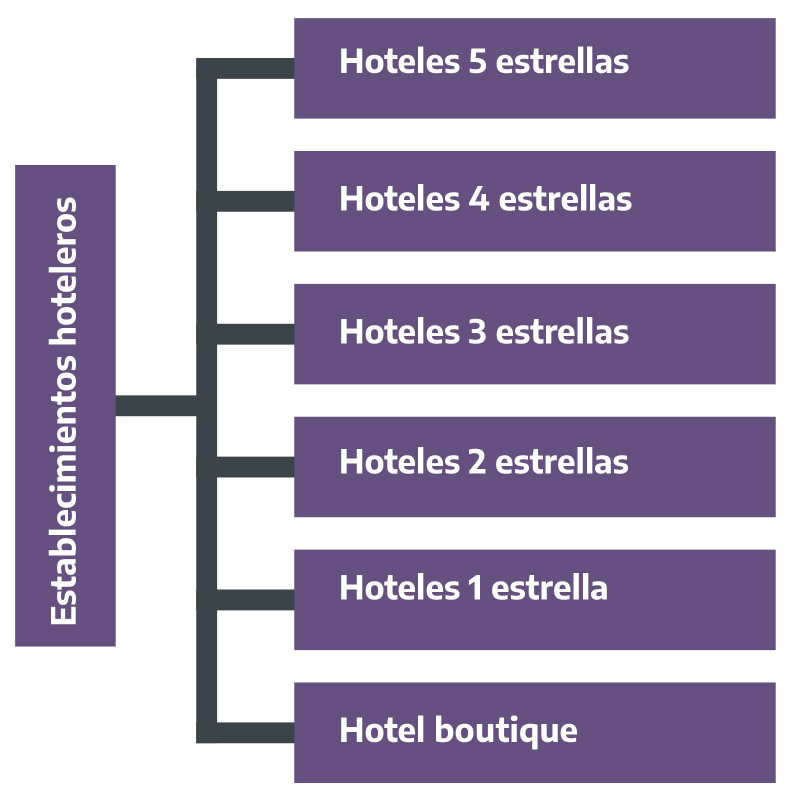
\includegraphics[width=1\linewidth]{imagenes/figura_3_1} 

}

\caption{Tipos de alojamientos turísticos. Establecimientos hoteleros}\label{fig:establecimientos-hoteleros}
\end{figure}

\begin{figure}

{\centering 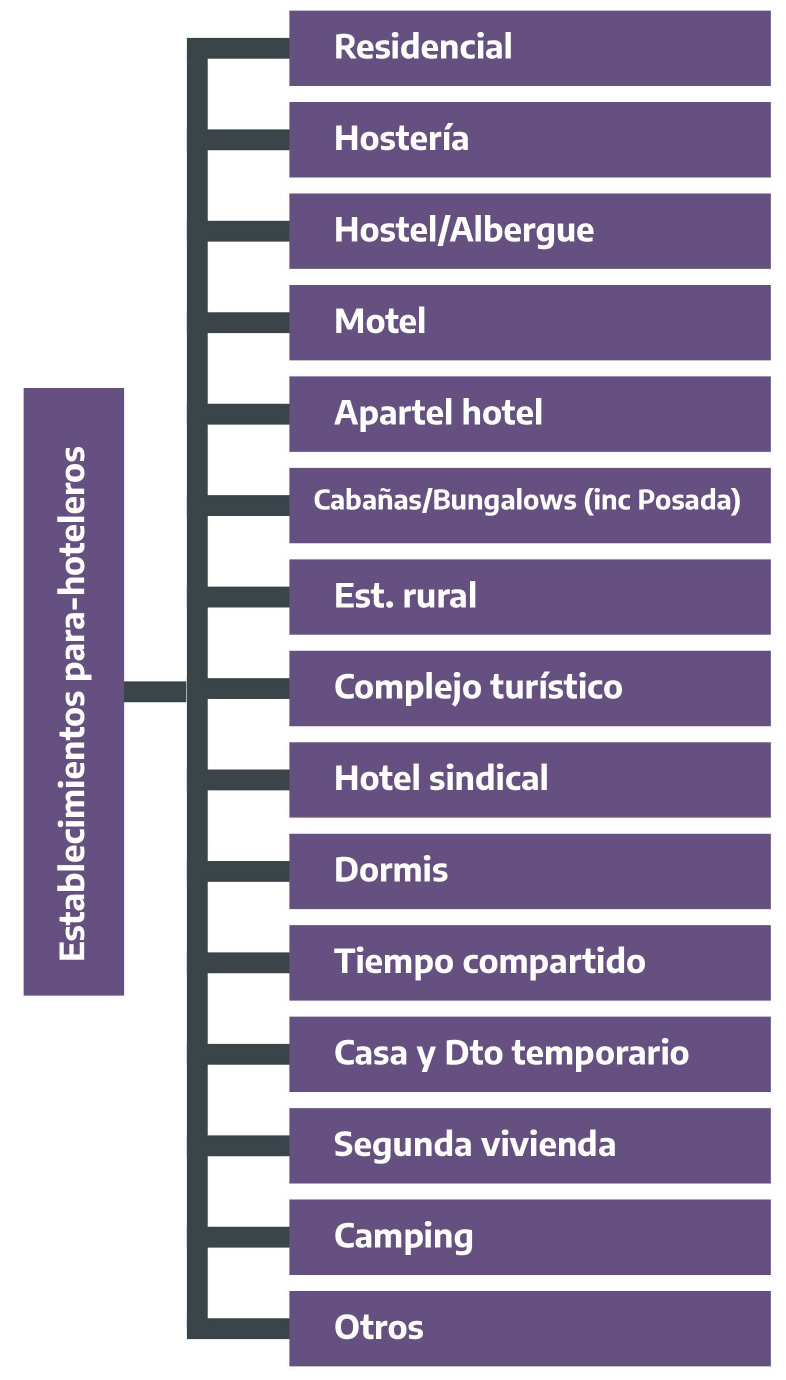
\includegraphics[width=1\linewidth]{imagenes/figura_3_2} 

}

\caption{Tipos de alojamientos turísticos. Establecimientos para-hoteleros}\label{fig:establecimientos-para-hoteleros}
\end{figure}

\hypertarget{trabajo-de-campo}{%
\section{Trabajo de campo}\label{trabajo-de-campo}}

\hypertarget{frecuencia-de-relevamiento-y-peruxedodo-de-referencia-de-los-datos-relevados}{%
\subsection{Frecuencia de relevamiento y período de referencia de los datos relevados}\label{frecuencia-de-relevamiento-y-peruxedodo-de-referencia-de-los-datos-relevados}}

El trabajo de campo (el momento del relevamiento de la información en sí), de forma similar a las otras etapas del estudio, también debe ser planificado de antemano, si bien en el transcurso del estudio pueden ir planteándose modificaciones.

Un punto importante es determinar la \textbf{periodicidad} con la que la información será recolectada, es decir, la frecuencia con la que se hará la toma del dato. Por ejemplo, dentro de un relevamiento continuo, es necesario definir si la recolección de los datos será mensual, quincenal, semanal, durante algunos días específicos de la semana o diaria. Lo mismo vale para un relevamiento puntual. Por ejemplo, en un operativo de temporada alta, es preciso determinar si los datos serán recolectados quincenalmente, semanalmente, durante algunos días específicos de la semana o diariamente.

Otro aspecto que merece ser definido con claridad es el \textbf{período de referencia} de los datos a relevarse. En otras palabras, debe establecerse a qué período estarán referidas las variables por las que se indagará. Este punto está fuertemente ligado a la frecuencia con la que se realice el relevamiento. En efecto:

\begin{itemize}
\item
  En los relevamientos diarios, el período de referencia de los datos relevados será el día anterior: por ejemplo, el martes se preguntará por la cantidad de plazas ocupadas del lunes; el miércoles por las del martes; el lunes por las del sábado y domingo (en este caso, se indagará por los dos días ya que los fines de semana no suelen ser días laborales).
\item
  En los relevamientos con frecuencia semanal, es preciso definir si se preguntará, por ejemplo, por las plazas ocupadas de cada día de la semana o de toda la semana. En este último caso, como la estimación de las plazas totales del período será tarea del respondente, deberían tomarse los recaudos necesarios para reducir al máximo las probabilidades de error de cálculo.
\item
  En los estudios con tomas de datos mensuales, las alternativas podrían ser solicitar datos por cada día del mes (situación más viable en relevamientos con entrevistas personales o con formularios autoadministrados) o por el período completo (todo el mes), lo cual conlleva a tomar los mismos recaudos que en los relevamientos semanales con datos referidos a toda la semana (por lo cual resulta la opción menos recomendable).
\item
  Por último, en los operativos que relevan datos más de una vez por semana, pero no todos los días, por ejemplo, los lunes y miércoles, es necesario establecer si se recabará información de todos los días previos a los días de relevamiento (lunes y martes) o de algún día específico del período previo, que se considere parecido al resto de los días no relevados.
\end{itemize}

La última alternativa citada resulta recomendable en relevamientos telefónicos que buscan reducir la frecuencia y duración de los llamados. Sin embargo, en caso de optar por ella, es preciso tener en cuenta que la definición de los días en que se realizará el relevamiento, así como también del día de referencia del dato relevado, no es un procedimiento automático. Por el contrario, supone un análisis y evaluación de las diferencias que podrían presentar las variables bajo estudio entre los diferentes días de la semana.

Cabe mencionar que, como se recabarán datos de dos o tres días de la semana, que luego deberán ser extrapolados al resto de los días, es imprescindible que los días sobre los que se relevarán datos (días de referencia) sean representativos de los días no relevados. Esto implica que los días de referencia deberán ser lo más parecidos posible a los días no relevados en función de las variables bajo análisis. Por tanto, un primer paso es la definición de los días de referencia. Para ello, es preciso analizar el comportamiento de las semanas y conformar grupos de días. Los días de cada grupo deberían ser lo más parecidos entre sí en función de las variables que serán medidas en el estudio; asimismo, cada grupo debe intentar diferenciarse lo más posible de los otros. En definitiva, se estarían definiendo estratos compuestos por días de la semana. A modo de ejemplo, podría suponerse, luego analizar datos provenientes de estudios previos, que los días domingo, lunes, martes, miércoles y jueves suelen manifestar un menor porcentaje de ocupación, así como una menor cantidad de ingresos de viajeros, que los días viernes y sábado. Por tanto, se conformarían dos grupos:

\begin{itemize}
\item
  Grupo A: días domingo, lunes, martes, miércoles y jueves.
\item
  Grupo B: días viernes y sábado.
\end{itemize}

Una vez establecidos los grupos de días, es necesario definir qué día de cada grupo se constituirá en día de referencia. Recuérdese que éste será el día sobre el cual se relevarán los datos, que luego serán extrapolados al resto de los días del grupo. La decisión de cuál será el día de referencia dependerá, en gran medida, del día en que pueda realizarse efectivamente el relevamiento y del funcionamiento operativo del equipo de estadísticas de la entidad de turismo. Supóngase que, por razones obvias, el equipo a cargo de las estadísticas de turismo no trabaje el fin de semana. Por tanto, los datos de cualquiera de los días del grupo B deberán ser relevados durante la semana. Lo más lógico es hacerlo un día cercano al día de referencia; por tanto, podría definirse al lunes como día en el que se relevarán los datos del sábado (día que será representativo de sí mismo y del viernes). En cuanto al grupo A, si ya se ha designado al lunes como día de relevamiento de información sobre el sábado, podría decidirse que el día de relevamiento del grupo A esté algo alejado del correspondiente al grupo B. Consecuentemente, los días miércoles o jueves podrían ser buenos candidatos a días de relevamiento del grupo A. Si, por ejemplo, se decidiese que el miércoles sea el elegido, lo más adecuado sería que el día de referencia sea el martes. En síntesis, en este caso hipotético, la conformación de los grupos sería la siguiente:

\begin{itemize}
\tightlist
\item
  \textbf{Grupo A:}
\end{itemize}

Día de relevamiento: miércoles.

Día de referencia: martes.

Días a los que se extrapolarán datos del martes: domingo, lunes, miércoles y jueves.

\begin{itemize}
\tightlist
\item
  \textbf{Grupo B:}
\end{itemize}

Día de relevamiento: lunes.

Día de referencia: sábado.

Días a los que se extrapolarán datos del sábado: viernes.

Ahora bien, una vez relevados los datos de los días martes y sábados, ¿cómo se extrapolan (o expanden) los datos al resto de los días? Supóngase que una de las variables relevadas es plazas ocupadas, y que en la semana X se obtienen los siguientes datos:

\begin{itemize}
\item
  Martes: 450 plazas ocupadas.
\item
  Sábado: 900 plazas ocupadas.
\end{itemize}

Si se expanden los datos del martes al resto de los días del grupo A, así como los datos del sábado al viernes, se obtiene lo siguiente:

\begin{figure}

{\centering 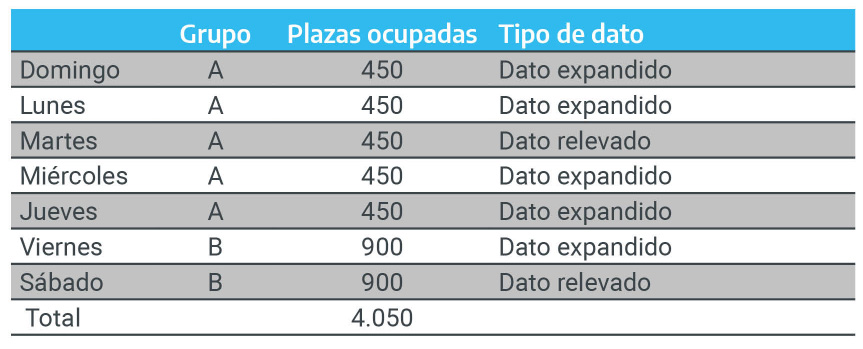
\includegraphics[width=1\linewidth]{imagenes/tabla_5a} 

}

\caption{Tabla de Grupos}\label{fig:grupo-a-b}
\end{figure}

Como puede observarse, a los días domingo, lunes, miércoles y jueves se les asignó la cantidad de plazas relevadas del día martes (450 plazas ocupadas), mientras que al viernes se expandió el dato del sábado (900 plazas ocupadas). Como resultado, el total de plazas ocupadas de la semana X es 4.050.

La EOH es un operativo contínuo desde el año 2004 con una frecuencia de relevamiento mensual y el periodo de referencia de los datos también es mensual. Es decir, todos los meses se le consulta a los establecimientos hoteleros y parahoteleros seleccionados información de la actividad de todo el mes. Diferente es lo que realiza la EOH de España, la cual presenta una frecuencia de relevamiento mensual pero el periodo de referencia es semanal: ``la consulta de datos básicos se refiere a siete días seguidos de cada mes, elegidos aleatoriamente, de tal manera que entre todos los establecimientos cubran el mes completo'' . Mayor información: \href{https://www.ine.es/daco/daco42/ocuphotel/notaeoh.htm}{Aquí}

A su vez, en Argentina, no sólo se le pregunta la cantidad de plazas y habitaciones ocupadas, de nuevos viajeros hospedados, las pernotaciones, sino también la disponibilidad de habitaciones, unidades y plazas y la cantidad de días abiertos en el mes de interés. Esto último es muy importante, por que algunos hoteles no abren sus puertas durante todo el mes, sino para determinadas fechas relevantes (un fin de semana largo por ejemplo) y por ello, la disponibilidad real del hotel se calculará en función de la disponibilidad de plazas/habitaciones/unidades que tiene ese hotel por la cantidad de días abiertos. Dicha información y, en función de los datos declarados de ocupación, se calculan las correspondientes tasas de ocupación mensuales durante todo el año.

\hypertarget{formas-de-relevamiento}{%
\subsection{Formas de relevamiento}\label{formas-de-relevamiento}}

Además de los aspectos desarrollados previamente, otro punto importante en la instancia de planificación del trabajo de campo es la evaluación de cuál será la \textbf{forma de relevamiento adecuada (telefónica, mediante entrevista personal}, \textbf{auto-administrada)}, teniendo en cuenta los objetivos, las dificultades propias del relevamiento, el tipo de estudio (censal o muestral), la celeridad con que se necesitan los resultados, los recursos humanos disponibles, la frecuencia de relevamiento, el período de referencia de los datos relevados, etc.

En la Figura 2.19 se presentan las ventajas, limitaciones y requerimientos de cada forma de relevamiento. Cabe mencionar que, a pesar de sus pros y contras, todas son alternativas válidas a la hora de ejecutar el trabajo de campo mientras se respeten los criterios metodológicos básicos que deben guiar el trabajo de campo.

\begin{figure}

{\centering 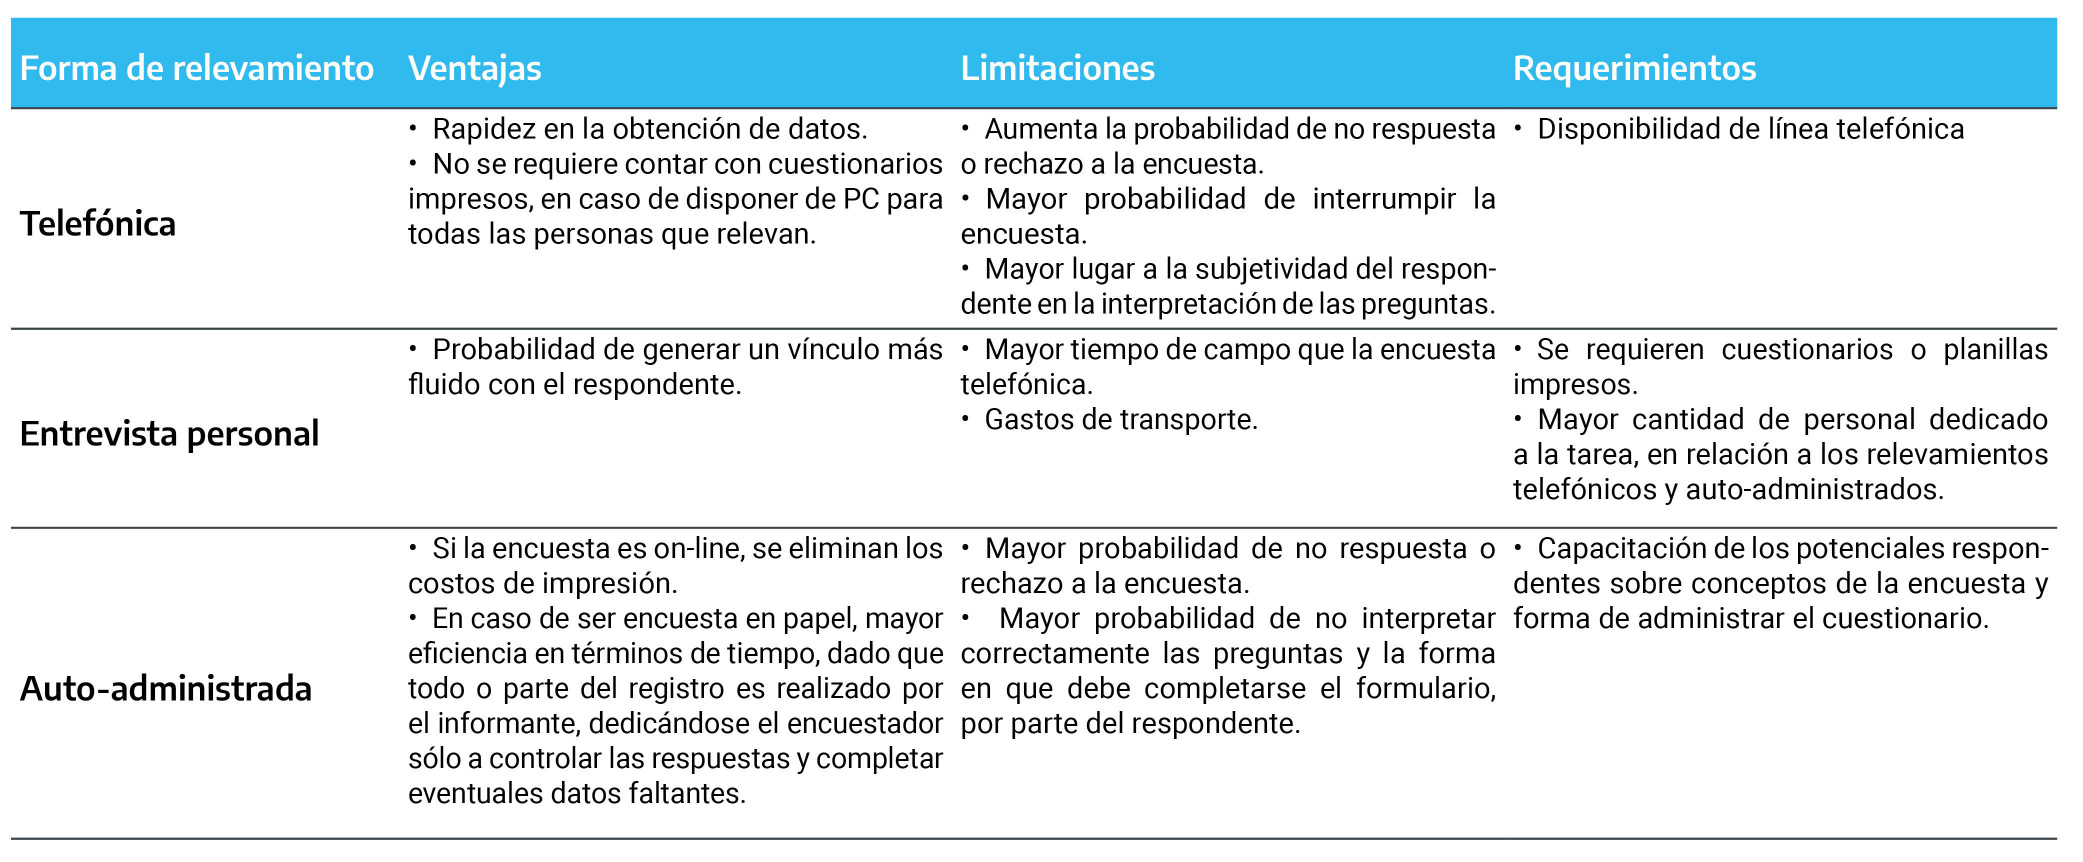
\includegraphics[width=1\linewidth]{imagenes/tabla_6} 

}

\caption{Ventajas, limitaciones y requerimientos por forma de relevamiento}\label{fig:relevamiento}
\end{figure}

\hypertarget{otras-consideraciones-acerca-del-trabajo-de-campo}{%
\subsection{Otras consideraciones acerca del trabajo de campo}\label{otras-consideraciones-acerca-del-trabajo-de-campo}}

En relación al personal a cargo de la recolección de datos, como se desprende de la figura anterior, las encuestas pueden ser realizadas por personas que trabajen dentro de la institución y que estén afectadas a distintas tareas, o por encuestadores específicamente destinados a este trabajo. En la mayoría de las jurisdicciones, por razones de disponibilidad de recursos humanos, el trabajo de campo es ejecutado por el mismo personal de las entidades de turismo.

Por último, es preciso llevar adelante un continuo y simultáneo monitoreo del trabajo de campo, dado que permite detectar a tiempo:

\begin{itemize}
\item
  si el relevamiento se finalizará en el tiempo estimado;
\item
  posibles errores de registro de los datos;
\item
  casos de no respuesta.
\end{itemize}

Si durante el trabajo de campo se detectan casos de no respuesta, y si se tratase de un estudio por muestreo, una alternativa posible sería el reemplazo probabilístico (esto es, con criterios aleatorios) del establecimiento sin dato por otro establecimiento de similares características.

\hypertarget{procesamiento-y-anuxe1lisis-de-la-informaciuxf3n}{%
\section{Procesamiento y análisis de la información}\label{procesamiento-y-anuxe1lisis-de-la-informaciuxf3n}}

La etapa lógica que sigue al trabajo de campo es la \textbf{carga de los datos}, que consiste en trasladar la información del cuestionario o planilla en papel a la base de datos. En las jurisdicciones que realizan relevamiento telefónico con ingreso directo de los datos en planillas digitales o softwares, la carga se efectúa, lógicamente, en simultáneo al trabajo de campo. En el caso de relevamientos online, muchos software permiten descargar los datos en formato de bases de datos.

Por otro lado, como se mencionó en el apartado 1.1, muchas provincias argentinas suelen recopilar datos de estudios de ocupación hotelera y para-hotelera producidos por los municipios. En varios de estos casos, los equipos técnicos de las provincias han diseñado planillas modelo en las que se propone a cada jurisdicción municipal cargar los datos producidos, con el fin de utilizarla para realizar estimaciones propias, ya sea a nivel local o provincial (agregando datos de las localidades relevadas).

A continuación se presenta un modelo de planilla para la carga de los datos, que puede ser utilizada por los municipios y/o provincias, ya sea para producir datos propios o recopilar datos producidos por terceros. Para seguir en la misma línea, se utilizaron algunos de los establecimientos considerados en el ejemplo de estratificación y selección de muestras al interior de cada estrato (apartado \protect\hyperlink{ejemplo-de-estratificaciuxf3n-y-selecciuxf3n-de-muestras-al-interior-de-cada-estrato}{Ejemplo de estratificación y selección de muestras al interior de cada estrato}). Asimismo, se asumió que el relevamiento se realiza los días lunes y miércoles, preguntando el lunes por las plazas ocupadas y plazas disponibles del sábado anterior, y el día miércoles por las plazas ocupadas del martes previo.

\begin{figure}

{\centering 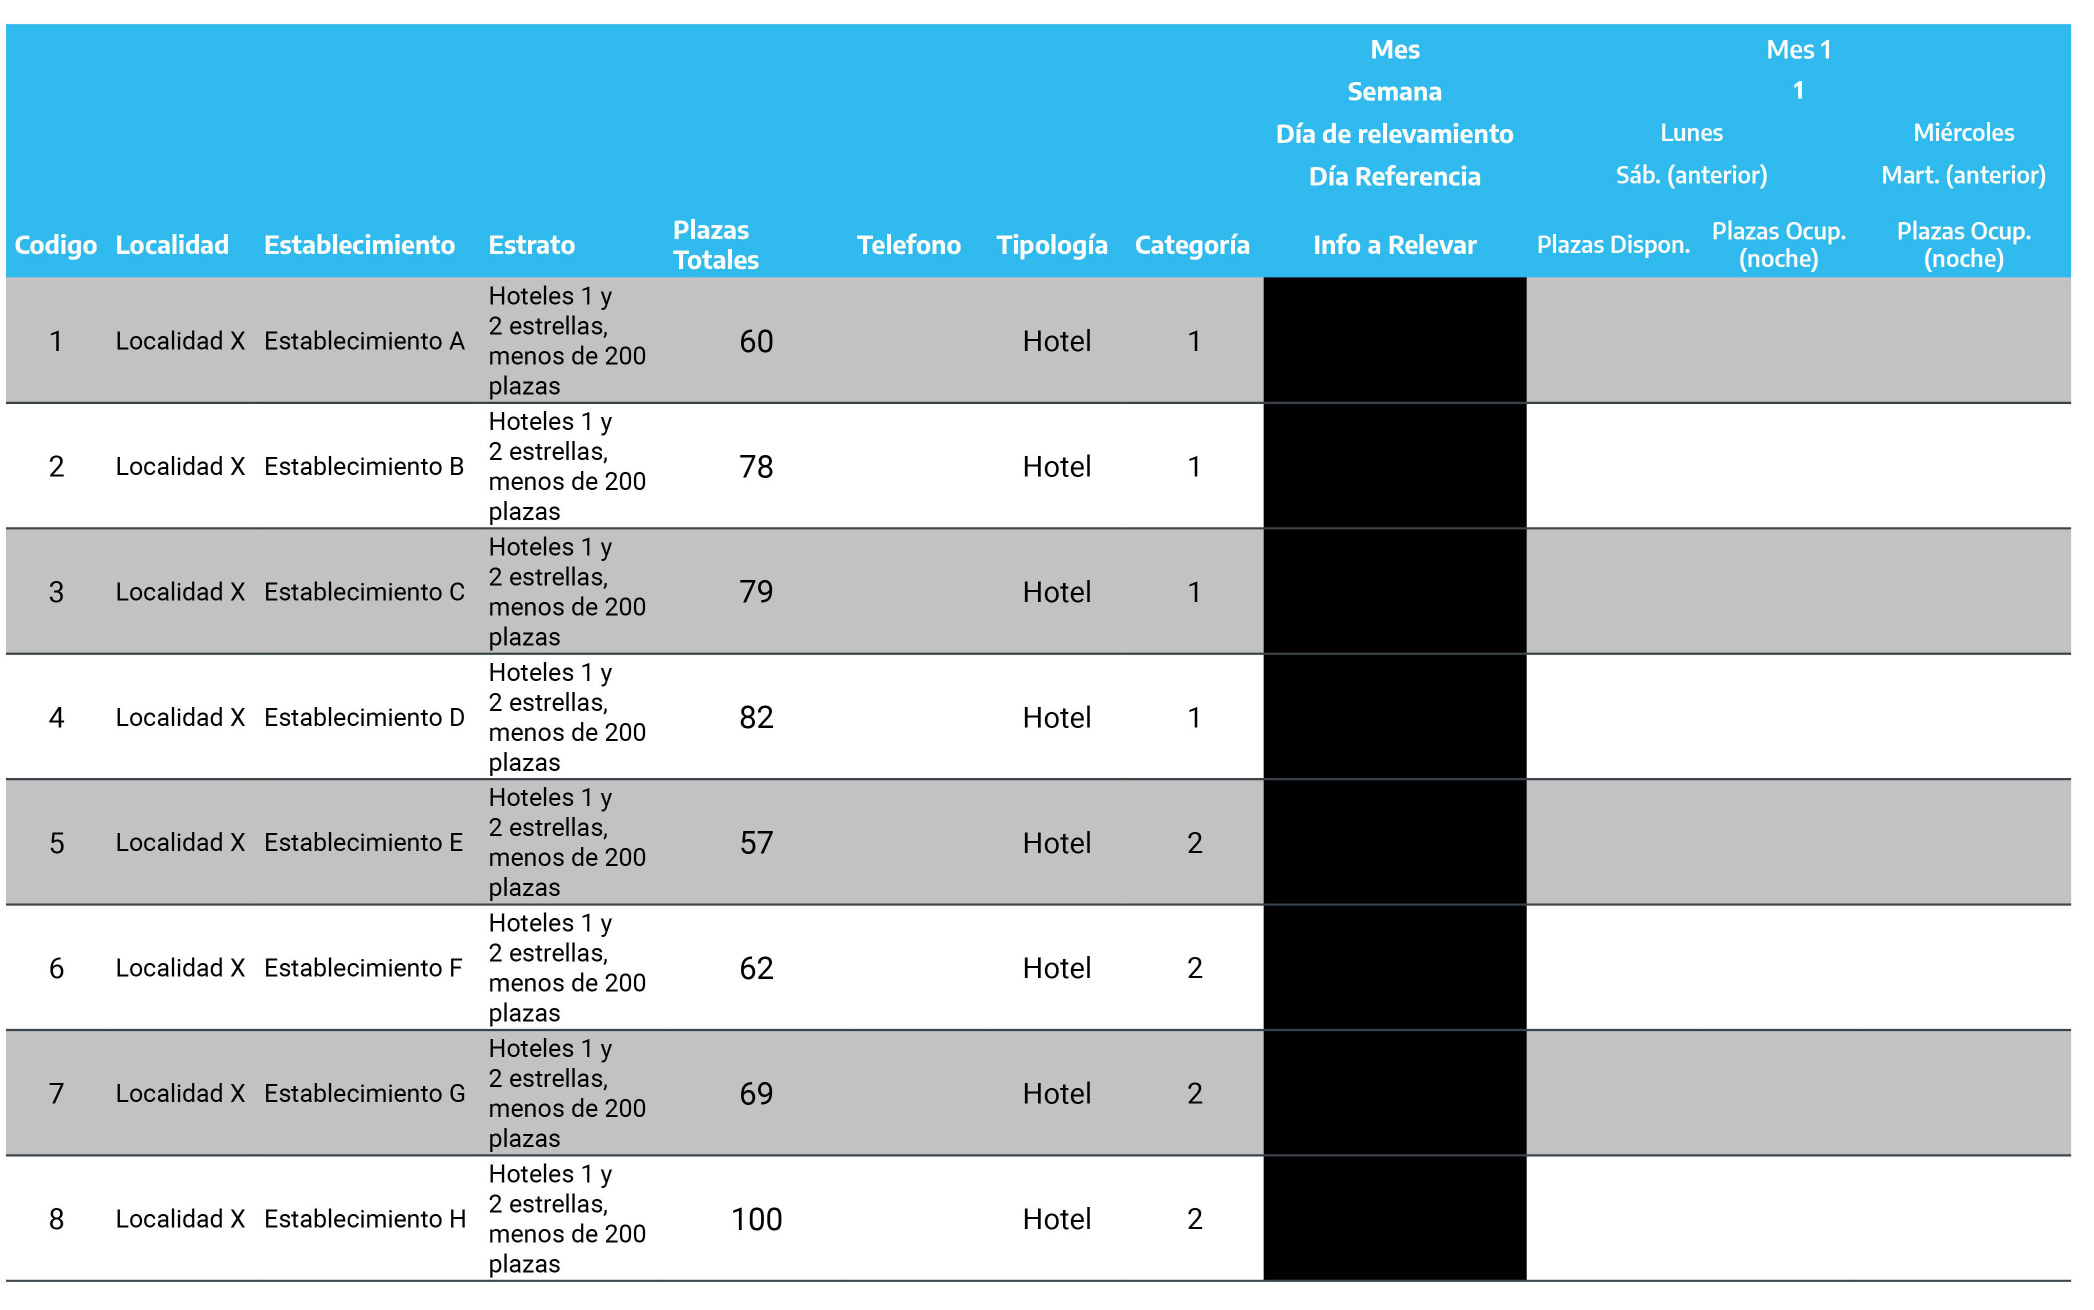
\includegraphics[width=1\linewidth]{imagenes/tabla_6a} 

}

\caption{Modelo de planilla para la carga de los datos}\label{fig:tabla-6a}
\end{figure}

\hypertarget{consistencia-y-validaciuxf3n-de-la-informaciuxf3n}{%
\subsection{Consistencia y validación de la información}\label{consistencia-y-validaciuxf3n-de-la-informaciuxf3n}}

Una vez que han sido ingresados los casos a la base de datos, es necesario llevar adelante un proceso de \textbf{validación}\footnote{La validación no es exclusiva de esta etapa y es preciso que se definan pautas de consistencia para las diferentes etapas del campo (cuando se completa el formulario, cuando el mismo es recepcionado por un supervisor, etc.). No obstante, en esta etapa las herramientas informáticas permiten validar la información en forma certera, pudiendo incluir además información externa (por ejemplo, si algún valor se aleja sustancialmente de la media del estrato o de información suministrada anteriormente por el mismo establecimiento, casos en los que es preciso chequear que la información brindada sea la correcta).}, lo cual implica realizar un análisis de consistencia interna de los datos y de situaciones extrañas o no esperadas en los valores de los datos. Durante la validación pueden detectarse \textbf{errores} y/o \textbf{advertencias}. Un ejemplo de error sería encontrar que la cantidad de plazas ocupadas supere a la cantidad de plazas disponibles\footnote{Sin embargo, puede ocurrir que un establecimiento, en períodos de alta demanda, utilice sus plazas supletorias. En esos casos, se debe corregir el número correspondiente a las plazas disponibles.}. Por otro lado, una advertencia se podría presentar cuando en un establecimiento se produce una variación notoria en la cantidad de plazas ocupadas, en un período en que se esperaba que ese valor estuviese estancado. Si durante el proceso de validación se detecta algún dato inconsistente o alguna advertencia, lo adecuado es volver a contactar al encuestado para solicitarle el dato correcto en el caso de un error o para constatar si lo que surgió como advertencia es un error o una situación que tuvo lugar realmente.

\hypertarget{tratamiento-de-la-no-respuesta}{%
\subsection{Tratamiento de la no respuesta}\label{tratamiento-de-la-no-respuesta}}

Otra situación que puede presentarse durante el proceso de chequeo de una base es la \textbf{ausencia de respuesta} (o no respuesta) en varias o todas las preguntas de algún caso específico. Si la no respuesta se reduce a algunas preguntas, la solución más atinada es, similarmente al caso anterior, intentar obtener el dato del mismo respondente. Si ello no fuese posible, un procedimiento válido es la \textbf{imputación}.

Imputar significa asignar a las preguntas con no respuesta valores provenientes de casos con características similares a las del caso en cuestión o, en estudios continuos, asignar valores del mismo caso en relevamientos anteriores (en lo posible, de similar período). Por ejemplo, si en un relevamiento continuo, un establecimiento X no informó la cantidad de habitaciones ocupadas en un período específico, y no se logra obtener el dato faltante por parte del informante, se puede optar por imputar el número de habitaciones ocupadas declarada por ese mismo establecimiento en un relevamiento previo que sea similar al evaluado, o bien aplicar el porcentaje de ocupación de uno o varios establecimientos similares (donante). Otra opción, quizás más sencilla que las anteriores (y siempre y cuando no haya sido posible obtener respuesta de los responsables de los alojamientos), es asignar a los establecimientos sin respuesta el valor promedio del estrato al que pertenecen. Por ejemplo, si en el estrato ``Hoteles 1 y 2 estrellas, menos de 200 plazas'' hay dos hoteles que no aportaron datos, y si en dicho estrato se obtuvo un \(74\%\) de ocupación, este procedimiento supone asignar a los establecimientos sin respuesta un \(74\%\) de ocupación.

\hypertarget{ponderadores-o-factores-de-expansiuxf3n}{%
\subsection{Ponderadores o factores de expansión}\label{ponderadores-o-factores-de-expansiuxf3n}}

Otro procedimiento clave, previo al análisis de los datos, es la construcción de \textbf{ponderadores} o, lo que es lo mismo, \textbf{factores de expansión}, que tienen una doble función y resultan ineludibles en todo estudio muestral:

\begin{itemize}
\tightlist
\item
  \textbf{Asignar a los casos relevados el mismo peso que tienen en el universo o población (calibrar).}
\end{itemize}

A menudo suele ocurrir, como producto de problemas inherentes al trabajo de campo (p.e., la no respuesta) o del mismo diseño muestral (en los estudios por muestreo), que algunos grupos o estratos (por ejemplo, clase, categoría, región, etc.) presenten en la muestra, o en el conjunto de casos relevados, un peso relativo diferente al que tenían en la población bajo estudio. En otras palabras, ya sea intencionalmente o como fruto de dificultades no controladas durante la fase de relevamiento, puede llegar a distorsionarse el peso de algunos grupos o estratos, quedando \textbf{sub} o \textbf{sobre-representados} en comparación con la población de origen. Por ejemplo, si en la población bajo estudio las plazas de los hoteles de 2 y 3 estrellas tienen una participación del \(30\%\), y en la muestra alcanzan un \(20\%\), esto significa que en la muestra este grupo de establecimientos se encuentra sub-representado (tiene un peso relativo inferior al que presenta en la población). Ante esta situación, se hace necesario \textbf{calibrar} o \textbf{corregir} la muestra (o conjunto de casos alcanzados), con el fin de devolver a cada grupo o estrato la participación relativa que tenían originalmente en la población bajo estudio. Esta será una de las funciones que tendrá el ponderador: multiplicar a cada uno de establecimientos de 2 y 3 estrellas relevados por un valor (ponderador), que permita transformar ese \(20\%\) muestral en un \(30\%\). En este caso, la fórmula para obtener el ponderador es dividiendo \(30\%\)/\(20\%\)=\(1,5\). Por lo tanto, a cada establecimiento de ese estrato hay que multiplicarlo por \(1,5\) para alcanzar el peso relativo original (\(30\%\)). Por otro lado, es probable que, si el estrato de 2 y 3 estrellas está sub-representado, otro estrato esté sobre-representado. Por lo tanto, los casos de este último deberán ser multiplicados por un valor inferior a 1, para ``aplastar'' el peso alcanzado por ese estrato en la muestra.

Para finalizar, se citará un ejemplo en el que se mostrará el peso original de cada grupo o estrato en la población y el peso alcanzado en la muestra; luego, se describirá el proceso de construcción de ponderadores para devolver, a cada estrato, el peso que originalmente exhibía en la población (en otras palabras, calibrar la muestra).

Se supone que la población bajo estudio está compuesta por hoteles de 1, 2, 3, 4 y 5 estrellas, agrupados en tres estratos, como se aprecia en la siguiente tabla.

\textbf{Estrato 1: hoteles de 1 estrella}

\(N1\)= \(15\);\(w\) (\(pow\))=\(0,3\);

\(n1\)= \(5\); \(w\) (\(muestra\))=\(0,2\).

\textbf{Estrato 2: hoteles de 2 y 3 estrellas}

\(N2\)= \(25\); \(w\) (\(pow\))=\(0,5\);

\(n2\)= \(10\);\$ w\$ (\(muestra\))=\(0,4\).

\textbf{Estrato 3: hoteles 4 y 5 estrellas}

N3= \(10\); \(w\) (\(pob\))=\(0,2\);

n3= \(10\); \(w\) (\(muestra\))=\(0,4\).

\textbf{Notaciones:}

\(N1,2,3\)=tamaño del estrato en la población

\(n1,2,3\)=tamaño del estrato en la muestra

\(w\) (pob)=peso del estrato en la población

\(w\) (muestra)= peso del estrato en la muestra.

En la tabla se observa que, en la muestra de establecimientos, los pesos que originalmente tenían cada estrato se han distorsionado. Cabe aclarar que, en algunos operativos, como es el caso de la EOH, el peso del estrato compuesto por hoteles de 4 y 5 estrellas se distorsiona intencionalmente, ya que se realiza un censo dentro del estrato. De todas formas, para que los resultados no se vean afectados, es preciso devolver a dicho estrato el peso original. Por lo tanto, para que cada uno de los estratos vuelva a contar con su peso original, se procede a construir los ponderadores de cada uno:

\textbf{Estrato 1 -} ponderador 1: \(0,3/0,2=1,5\)

\textbf{Estrato 2 -} ponderador 2: \(0,5/0,4=1,25\)

\textbf{Estrato 3 -} ponderador 3: \(0,2/0,4=0,5\)

\textbf{En consecuencia, a los casos del estrato 1 se los debe multiplicar por} \(1,5\)\textbf{; a los del estrato 2 por} \(1,25\)\textbf{; y a los del estrato 3 por} \(0,5\)

Los cálculos realizados son una simplificación, ya que además de calibrar, un ponderador también debe cumplir la función de expandir los resultados de la muestra al total poblacional, tal como se describe debajo.

\begin{itemize}
\tightlist
\item
  \textbf{Expandir los resultados} obtenidos sobre los casos relevados a todo el universo (factor de expansión inicial). Esto es, si el universo contempla 100 establecimientos y se encuesta a 20 de ellos, los resultados de cada establecimiento relevados deberán multiplicarse por 5 (\(100/20=5\)) para representar los valores del universo bajo estudio. En el caso de un muestreo estratificado, este coeficiente debe ser calculado para cada estrato.
\end{itemize}

Nuevamente, si bien su función es doble, esto no significa que haya que calcular un ponderador para expandir y otro para calibrar. Por el contrario, un mismo ponderador cumple esta doble tarea. En definitiva, los factores de expansión son números (fraccionarios o enteros) por los que se multiplican a los casos reales para lograr el doble propósito que se describió arriba. En general, en los estudios por muestreo se suele calcular un factor de expansión o ponderador \textbf{inicial} en la etapa de selección de la muestra, es decir previo al trabajo de campo. Luego del trabajo de campo, si se produjesen desajustes de los casos (sobre o sub representación de los casos), se procede a ajustar el factor de expansión inicial, para, además de expandir, calibrar los resultados.

Cabe mencionar que los procedimientos para el cálculo de ponderadores presentados son aplicables a muestras seleccionadas con las técnicas MAS o MSYS, en las cuales cada uno de los elementos tiene idéntica probabilidad de selección.

Para afianzar las ideas desarrolladas en este apartado, a continuación se describirá el proceso de construcción de factores de expansión para las muestras seleccionadas en el apartado \protect\hyperlink{trabajo-de-campo}{Trabajo de campo}

Recuérdese que la muestra final seleccionada fue:

\begin{figure}

{\centering 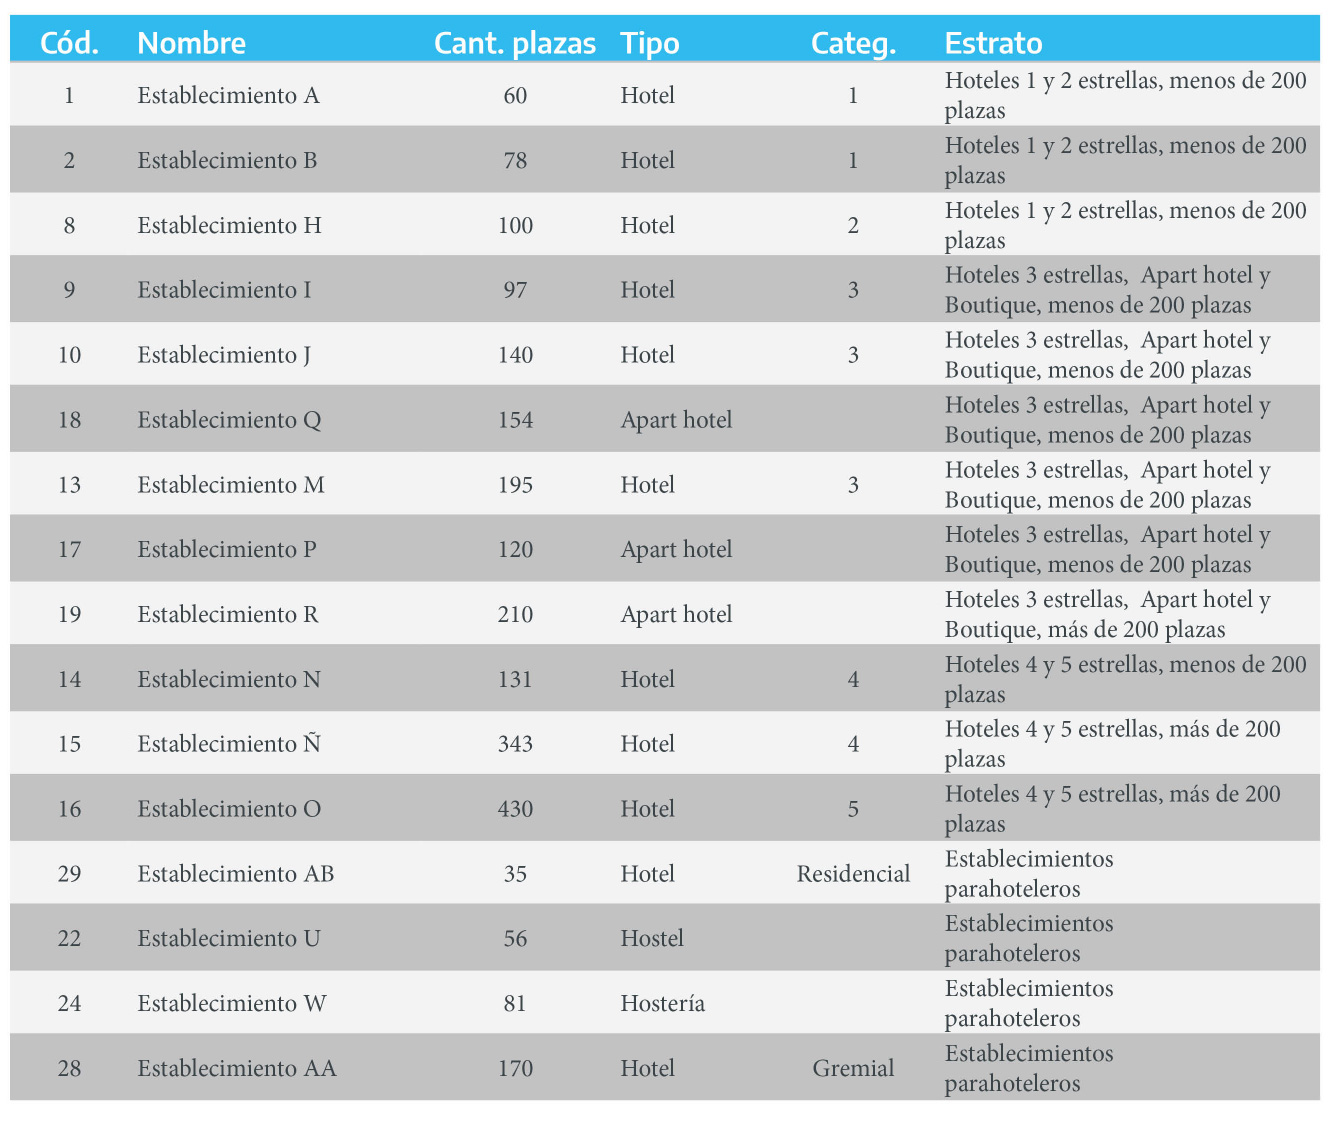
\includegraphics[width=1\linewidth]{imagenes/tabla_7a} 

}

\caption{Muestra final}\label{fig:tabla-7a}
\end{figure}

En primer lugar, los establecimientos de los estratos ``Hoteles 4 y 5 estrellas, menos de 200 plazas'' y ``Hoteles 4 y 5 estrellas, más de 200 plazas'' tienen un ponderador con valor 1, ya que han sido seleccionados todos los establecimientos y, por tanto, no es necesario expandir los resultados que se obtengan a ningún otro establecimiento. En otras palabras, los establecimientos de estos estratos están ``auto-representados'' . Lo mismo ocurre con el establecimiento del estrato ``Hoteles 4 y 5 estrellas, más de 200 plazas'': su ponderador es 1, y por tanto está auto-representado.

¿Cuál es el procedimiento para el cálculo de los ponderadores en resto de los estratos?

La variable que se utilizará para el cálculo de los factores de expansión de cada estrato será ``cantidad de plazas disponibles'' , ya que en base a la misma se llevó adelante el procedimiento de selección de la muestra. Por tanto, debajo se describen los cálculos para obtener los ponderadores iniciales de cada estrato.

\textbf{Hoteles 1 y 2 estrellas, menos de 200 plazas:}

\begin{itemize}
\item
  Cantidad de plazas disponibles totales del estrato: \(587\).
\item
  Cantidad de plazas disponibles de la muestra: \(238\).
\item
  Ponderador: \(587/238=2,46638\)
\item
  \textbf{Hoteles 3 estrellas, Apart hotel y Boutique, menos de 200 plazas:}
\item
  Cantidad de plazas disponibles totales del estrato: \(1.056\).
\item
  Cantidad de plazas disponibles de la muestra: \(706\).
\item
  Ponderador: \(1.056/706=1,49575\)
\end{itemize}

\textbf{Establecimientos parahoteleros:}

\begin{itemize}
\item
  Cantidad de plazas disponibles totales del estrato: \(811\).
\item
  Cantidad de plazas disponibles de la muestra: \(342\).
\item
  Ponderador: \(811/342=2,37134\)
\end{itemize}

Como se ve, en el estrato ``Hoteles 1 y 2 estrellas, menos de 200 plazas'' el ponderador tiene un valor de 2,46638. Si a las plazas de cada establecimiento seleccionado en la muestra (de este estrato) se las multiplica por este valor, y luego se las suma, se obtiene eltotal de plazas del estrato: 587.Lo mismo ocurre con los otros estratos. Para que se comprenda gráficamente esta idea, en la tabla que sigue se realiza la operación mencionada para cada estrato.

\begin{figure}

{\centering 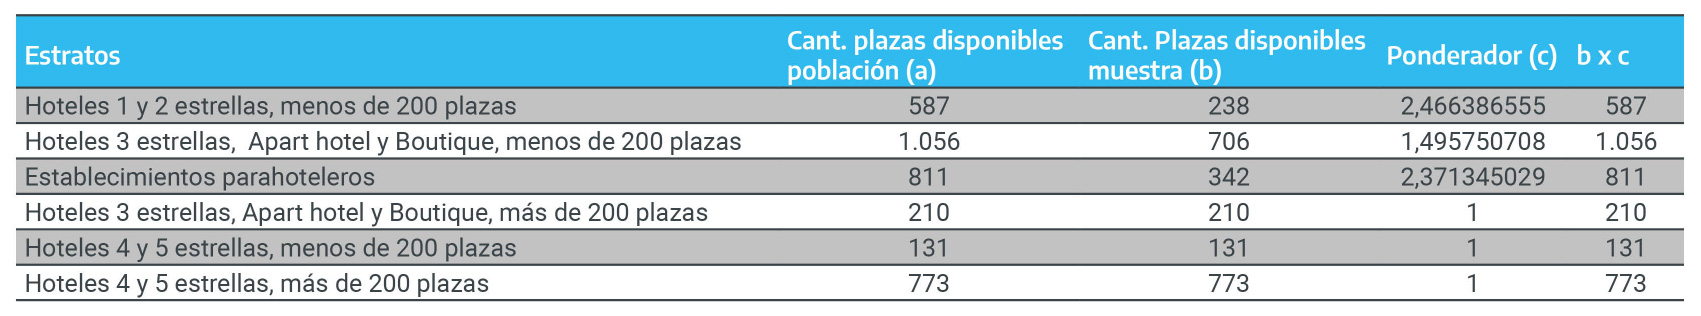
\includegraphics[width=1\linewidth]{imagenes/tabla_7b} 

}

\caption{Ponderadores}\label{fig:tabla7A}
\end{figure}

\hypertarget{obtenciuxf3n-de-resultados}{%
\section{Obtención de resultados}\label{obtenciuxf3n-de-resultados}}

Una vez finalizado el proceso de validación y construidos los factores de expansión, se está en condiciones de \textbf{calcular los indicadores} que respondan a los objetivos de investigación.

A continuación se presentan algunas alternativas de cálculo de los principales indicadores que usualmente se pretenden estimar a través de los relevamientos de alojamientos turísticos.

Cabe indicar que por razones de simplicidad, los ``totales'' que se mencionan surgirían, si se tratara de un estudio muestral, de los resultados ya expandidos.

\begin{figure}

{\centering 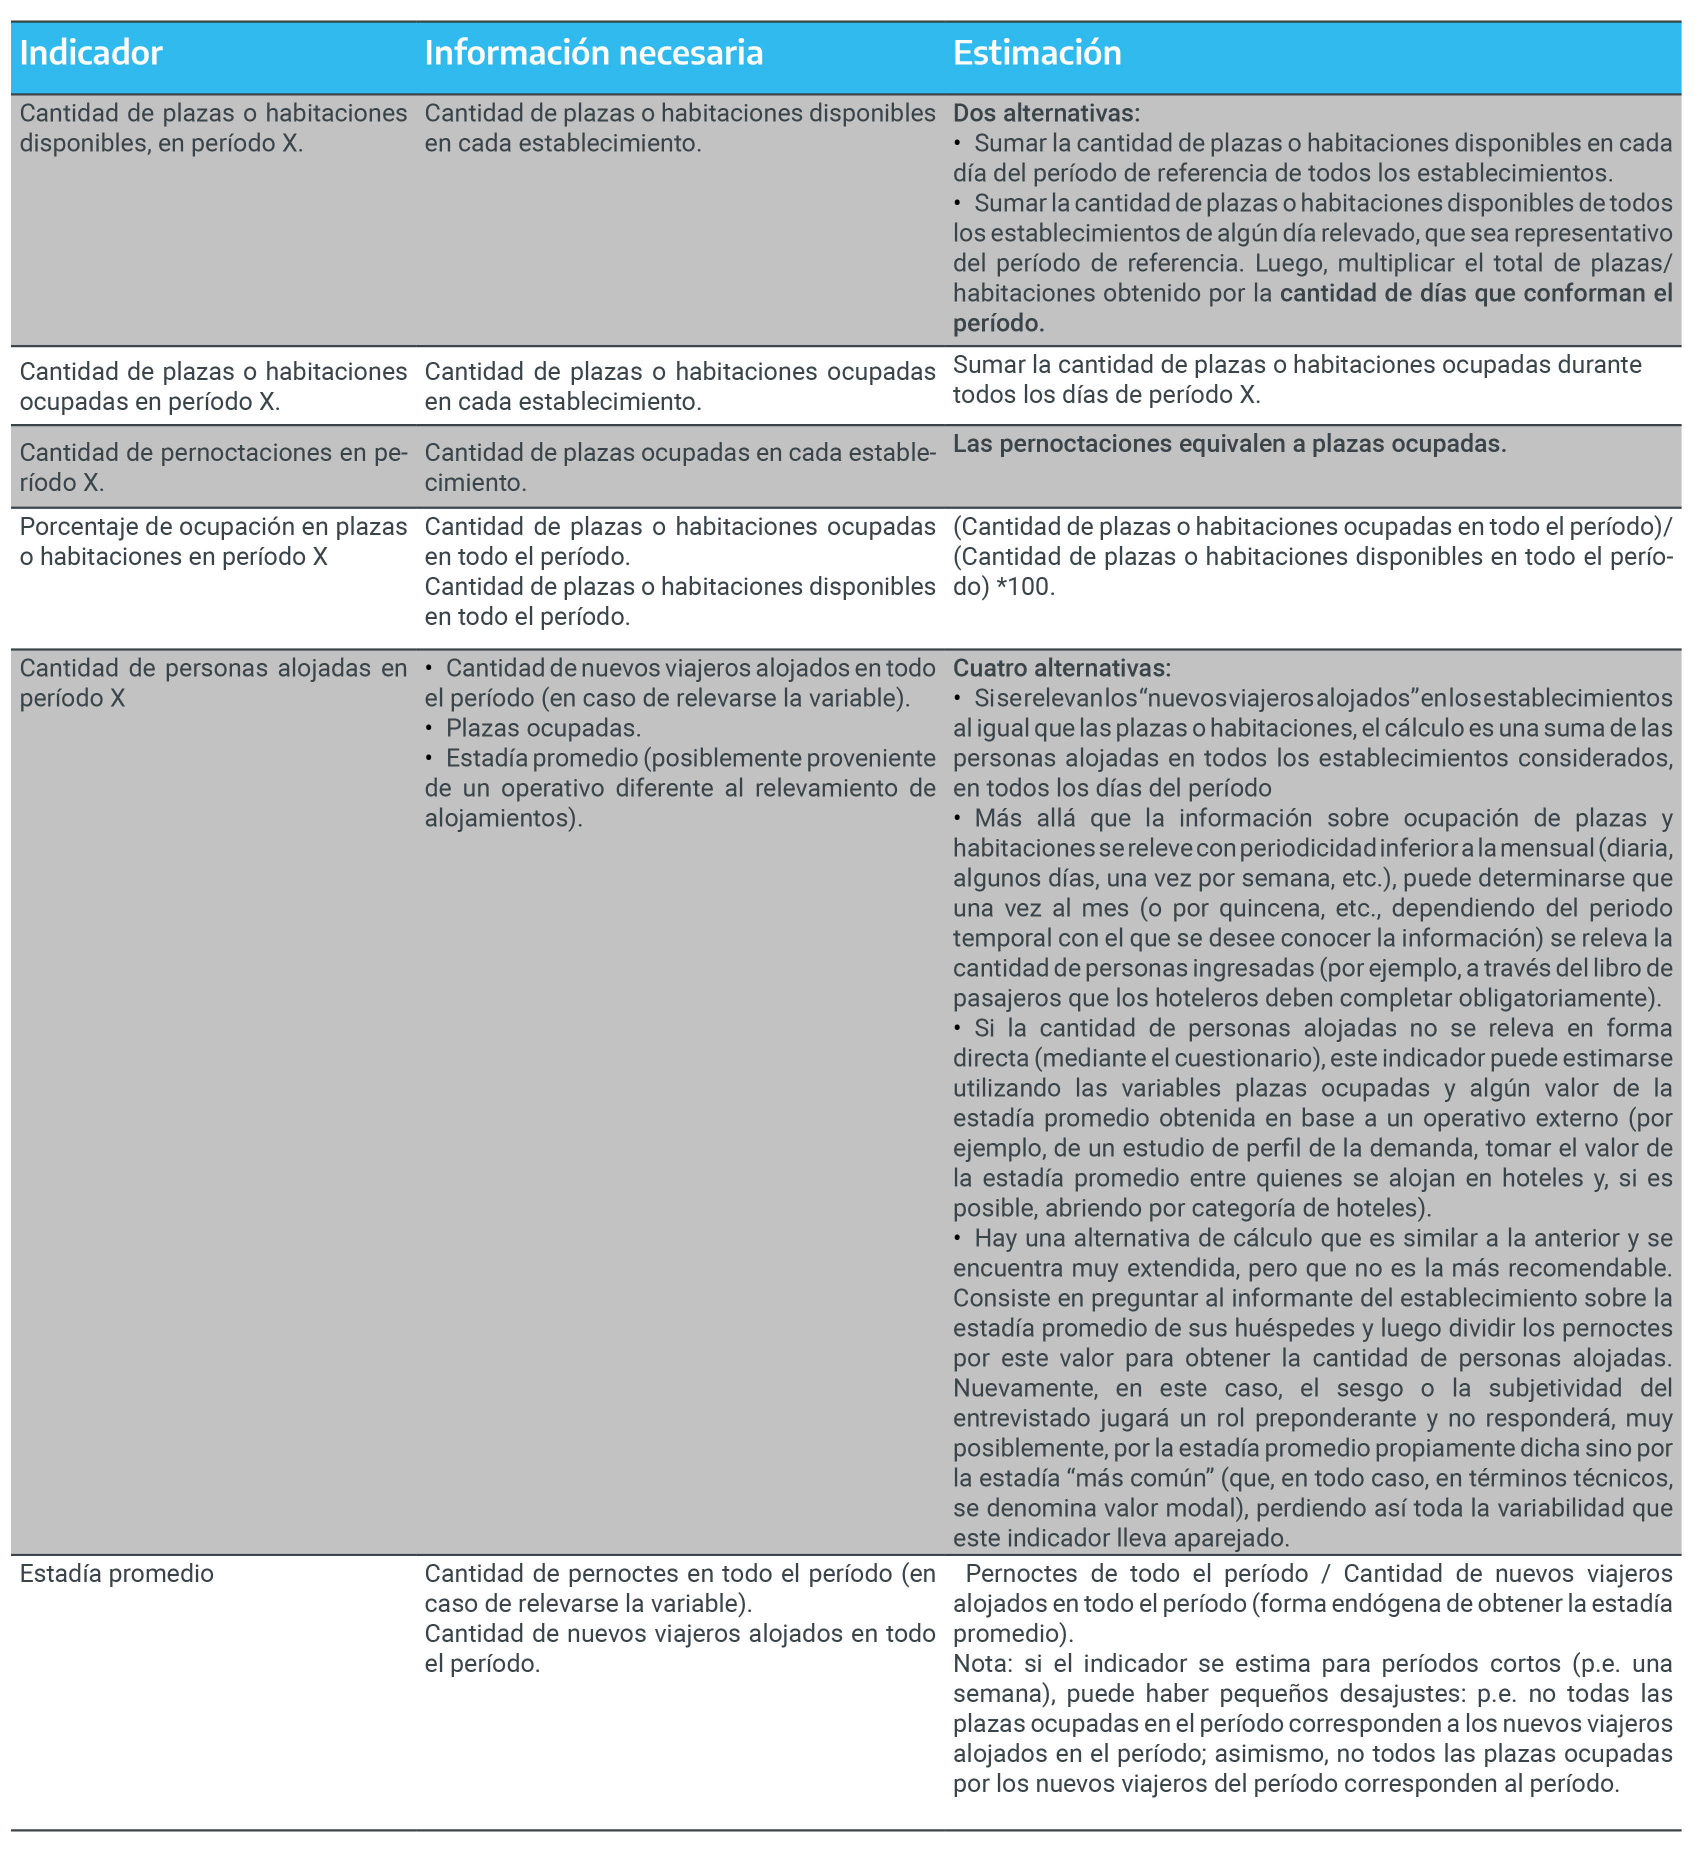
\includegraphics[width=1\linewidth]{imagenes/tabla_8} 

}

\caption{Indicadores, información necesaria para su construcción y procedimiento de estimación}\label{fig:indicadores}
\end{figure}

Para concluir este apartado, se retomará el ejemplo aplicado en los apartados 2.5.2.8 y 2.9.3 para el cálculo de los indicadores \textbf{``cantidad de plazas ocupadas (o pernoctaciones)''} y \textbf{``porcentaje de ocupación en plazas''}.

Cabe recordar que el objetivo de la Provincia X es obtener resultados para el total de la Localidad Y, sin realizar aperturas por estrato. Sin embargo, para obtener los resultados agregados, es preciso realizar previamente algunos cálculos en cada uno de los estratos.

En cada una de las tablas que siguen, en donde se realizan los cálculos por estrato, se presenta la siguiente información:

\begin{itemize}
\item
  \textbf{``Cantidad de plazas totales''}: son las plazas disponibles por establecimiento que figuran en el padrón.
\item
  \textbf{``Cantidad de plazas disponibles en la semana 1 (a)''}: es el resultado de multiplicar, para cada establecimiento, las plazas disponibles en el padrón por la cantidad de días del período de referencia. Esto último solo es posible si, en el período bajo estudio, ninguno de los establecimientos presenta variaciones en la oferta de plazas\footnote{Recuérdese que en algunas jurisdicciones la cantidad de plazas y/o habitaciones ofrecidas pueden sufrir variaciones (aumentos o bajas) a lo largo del año.}. En este sentido, lo recomendable es relevar, con una frecuencia establecida, la cantidad de plazas disponibles en cada establecimiento relevado, con el fin de detectar posibles variaciones en la oferta.
\item
  \textbf{``Cantidad de plazas ocupadas en la semana 1 (b)''}: es un dato obtenido del propio relevamiento.
\item
  \textbf{``Ponderador (c)''}: es el valor que se ha calculado en el apartado 2.9.3, para cada estrato.
\item
  \textbf{``Cantidad de plazas disponibles semana 1 en todo el estrato (d)''}: es el total de plazas disponibles del estrato (es decir, considerando la totalidad de los establecimientos) multiplicado por la cantidad de días del período de referencia.
\end{itemize}

\textbf{``Cantidad de plazas ocupadas semana 1-dato expandido (e)''}: se obtiene multiplicando la cantidad de plazas ocupadas de cada establecimiento por el ponderador del estrato.

\begin{figure}

{\centering 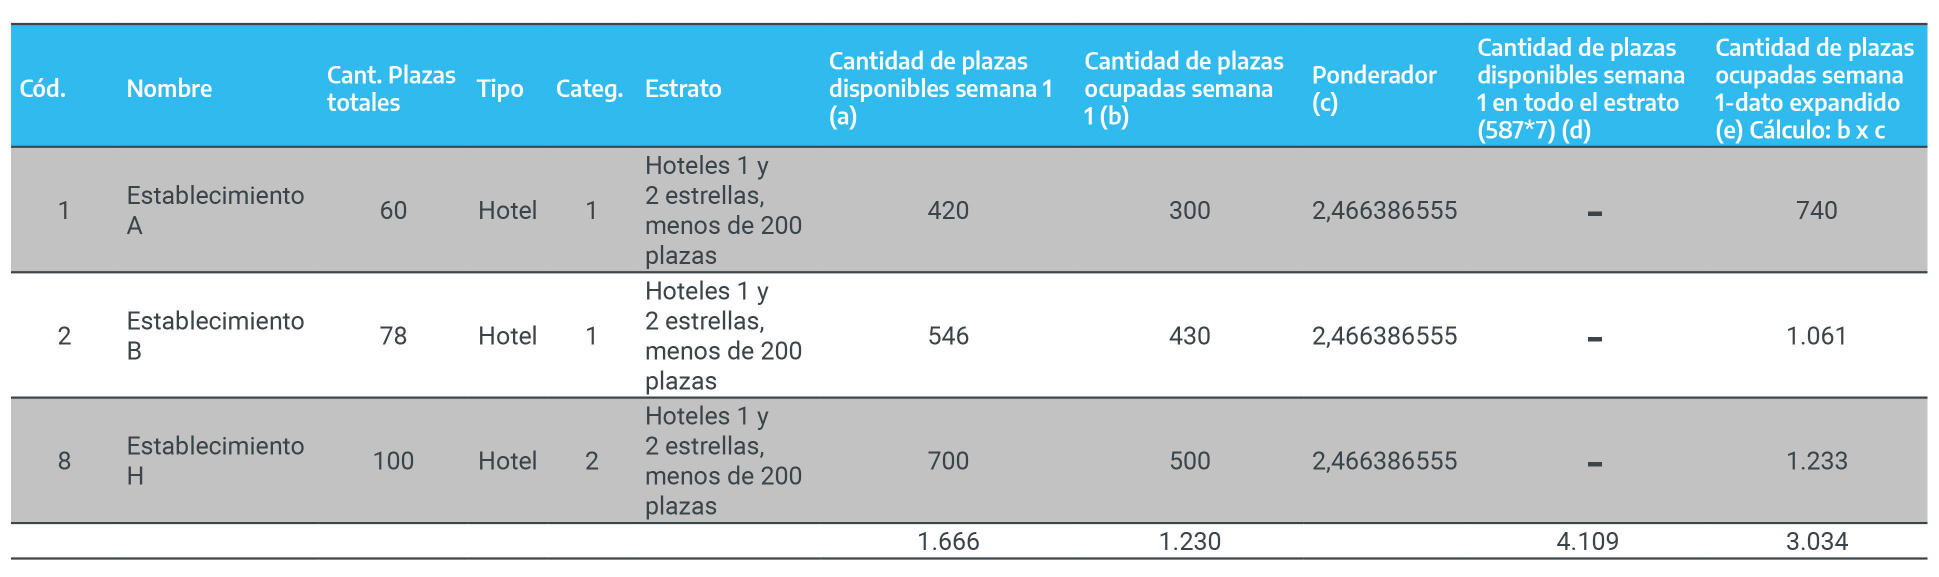
\includegraphics[width=1\linewidth]{imagenes/hoteles1y2_estrellas_menos_de_200_plazas} 

}

\caption{Hoteles 1 y 2 estrellas, menos de 200 plazas}\label{fig:1-2-estrellas}
\end{figure}

\begin{figure}

{\centering 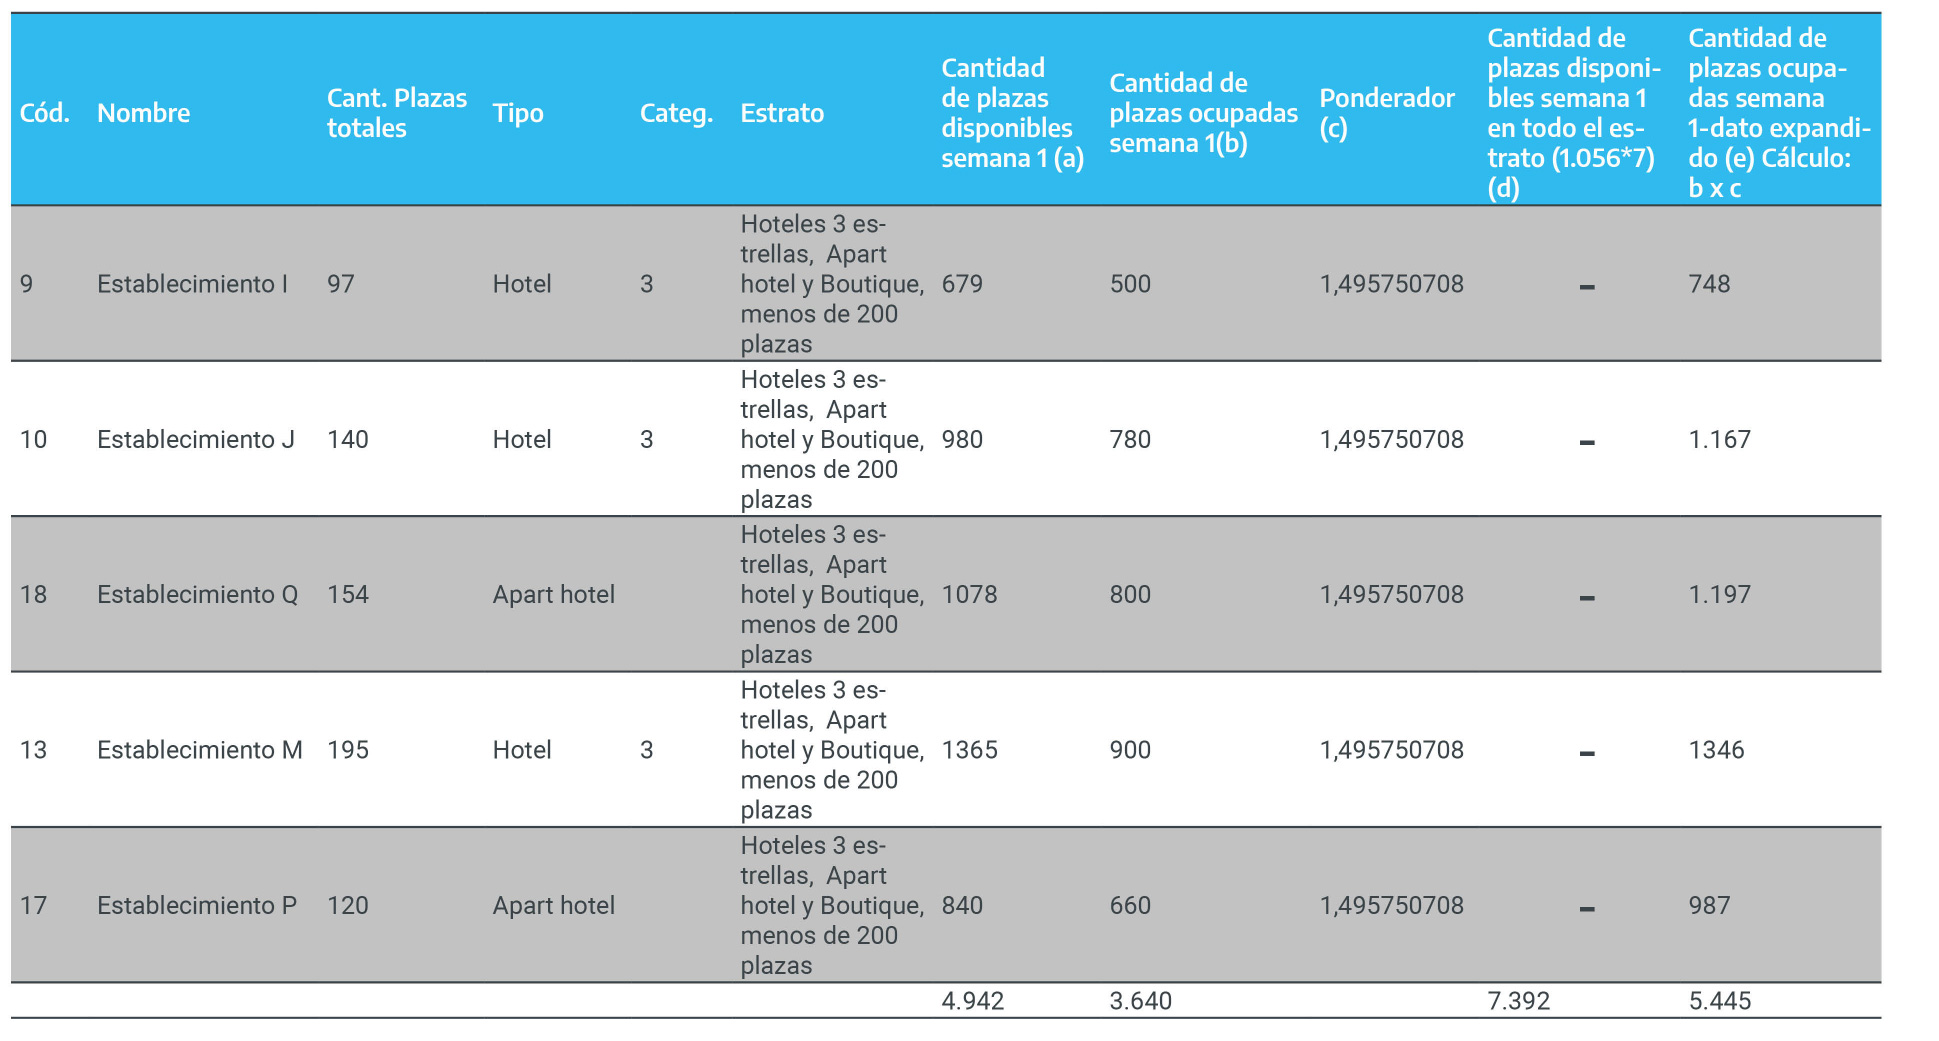
\includegraphics[width=1\linewidth]{imagenes/hoteles3_estrellas_apart_boutique_menos_200_plazas} 

}

\caption{Hoteles 3 estrellas,  Apart hotel y Boutique, menos de 200 plazas}\label{fig:3-estrellas}
\end{figure}

\begin{figure}

{\centering 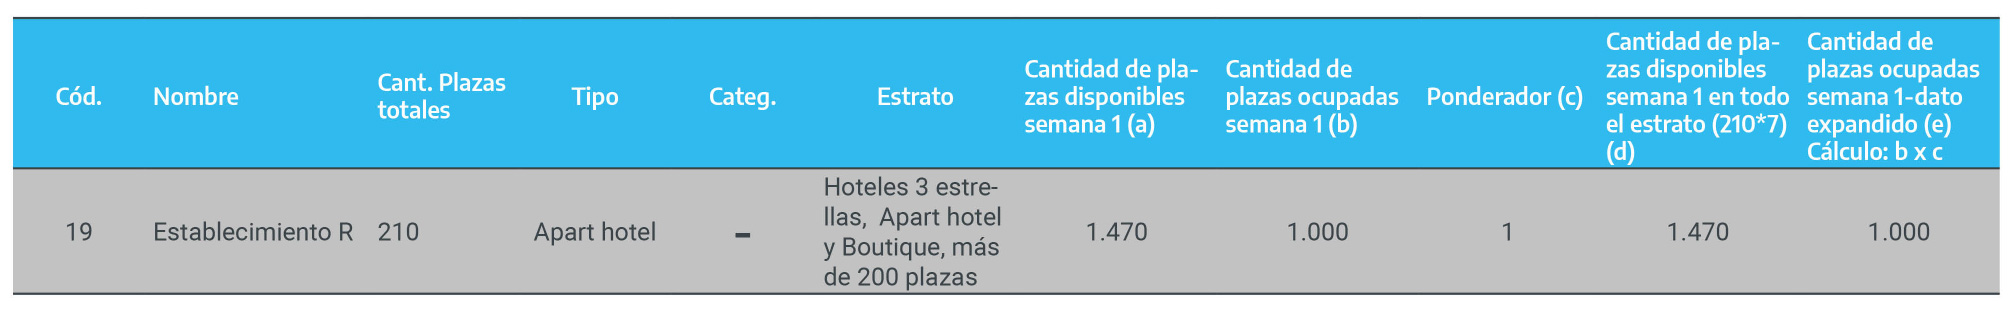
\includegraphics[width=1\linewidth]{imagenes/hoteles3_estrellas_apart_boutique_mas_200_plazas} 

}

\caption{Hoteles 3 estrellas,  Apart hotel y Boutique, más de 200 plazas}\label{fig:3-estrellas-mas200}
\end{figure}

\begin{figure}

{\centering 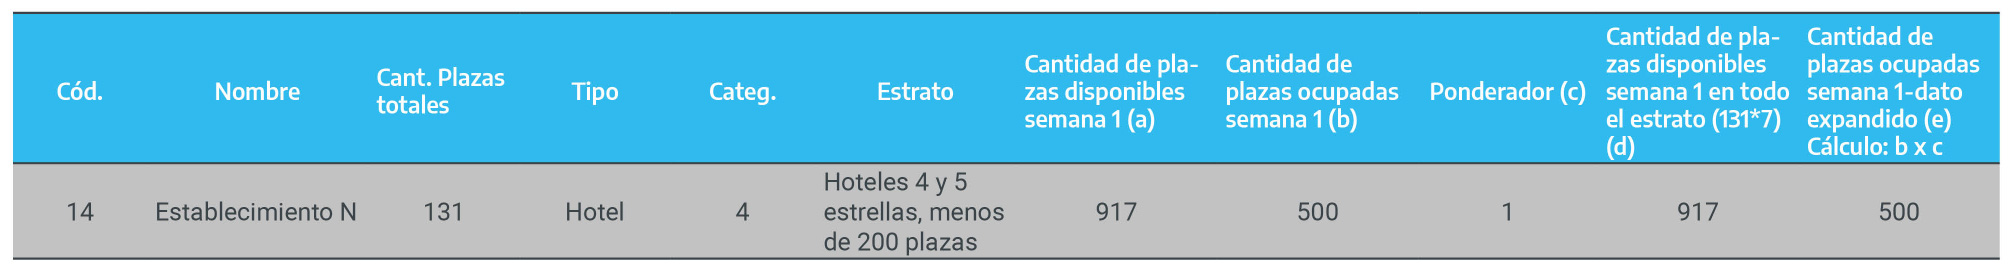
\includegraphics[width=1\linewidth]{imagenes/hoteles4_5_estrellas_menos_200_plazas} 

}

\caption{Hoteles 4 y 5 estrellas, menos de 200 plazas}\label{fig:4-5-estrellas-menos200}
\end{figure}

\begin{figure}

{\centering 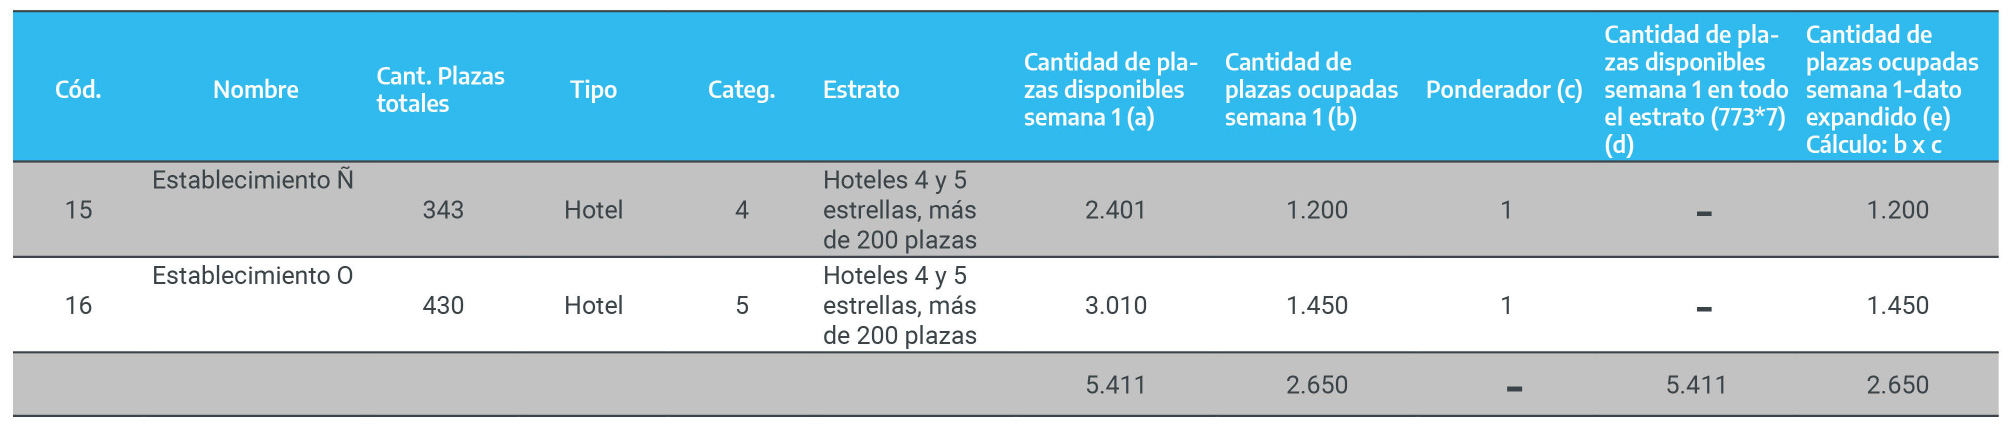
\includegraphics[width=1\linewidth]{imagenes/hoteles4_5_estrellas_mas_200_plazas} 

}

\caption{Hoteles 4 y 5 estrellas, más de 200 plazas}\label{fig:4-5-estrellas-mas200}
\end{figure}

\begin{figure}

{\centering 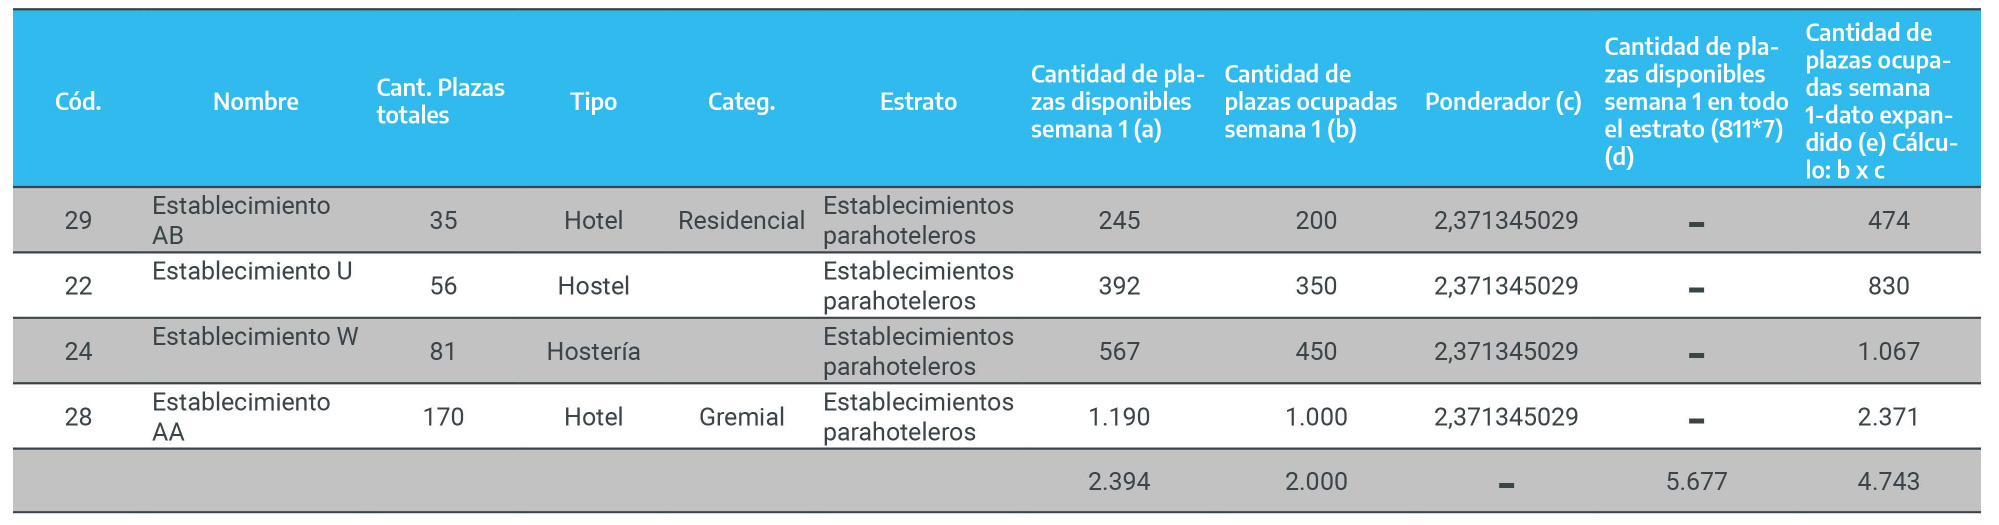
\includegraphics[width=1\linewidth]{imagenes/establecimientos_parahoteleros} 

}

\caption{Establecimientos parahoteleros}\label{fig:para-hoteleros}
\end{figure}

Luego de haber realizado los cálculos previos por estrato, se procede a estimar los indicadores para el total de la Localidad Y.

\begin{figure}

{\centering 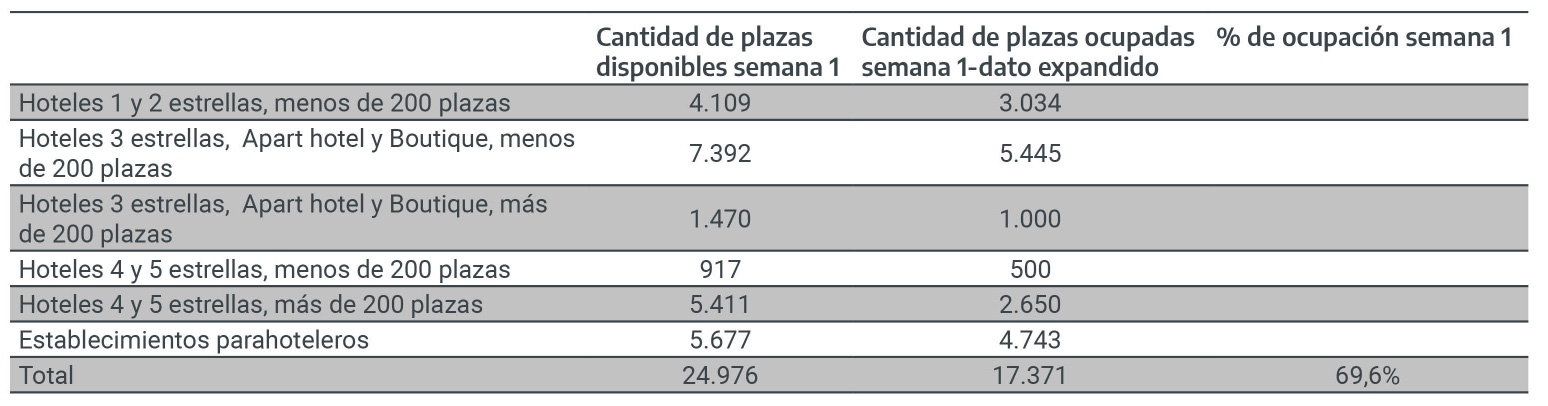
\includegraphics[width=1\linewidth]{imagenes/figuras_parte123_01} 

}

\caption{Total localidad}\label{fig:total-localodad-y}
\end{figure}

Como puede observarse, la cantidad de plazas ocupadas (o pernoctaciones) totales de la Localidad Y, en la semana 1, son el resultado de la suma de las plazas ocupadas de todos los estratos, habiendo aplicado previamente los correspondientes factores de expansión. Por otra parte, el porcentaje de ocupación total, en la semana 1, es la razón entre la cantidad de plazas ocupadas (o pernoctaciones) totales (17.371) y la cantidad de plazas disponibles totales (24.976).

  \bibliography{book.bib,packages.bib}

\end{document}
